\documentclass[twoside]{book}

% Packages required by doxygen
\usepackage{calc}
\usepackage{doxygen}
\usepackage{graphicx}
\usepackage[utf8]{inputenc}
\usepackage{makeidx}
\usepackage{multicol}
\usepackage{multirow}
\usepackage{textcomp}
\usepackage[table]{xcolor}

% Font selection
\usepackage[T1]{fontenc}
\usepackage{mathptmx}
\usepackage[scaled=.90]{helvet}
\usepackage{courier}
\usepackage{amssymb}
\usepackage{sectsty}
\renewcommand{\familydefault}{\sfdefault}
\allsectionsfont{%
  \fontseries{bc}\selectfont%
  \color{darkgray}%
}
\renewcommand{\DoxyLabelFont}{%
  \fontseries{bc}\selectfont%
  \color{darkgray}%
}

% Page & text layout
\usepackage{geometry}
\geometry{%
  a4paper,%
  top=2.5cm,%
  bottom=2.5cm,%
  left=2.5cm,%
  right=2.5cm%
}
\tolerance=750
\hfuzz=15pt
\hbadness=750
\setlength{\emergencystretch}{15pt}
\setlength{\parindent}{0cm}
\setlength{\parskip}{0.2cm}
\makeatletter
\renewcommand{\paragraph}{%
  \@startsection{paragraph}{4}{0ex}{-1.0ex}{1.0ex}{%
    \normalfont\normalsize\bfseries\SS@parafont%
  }%
}
\renewcommand{\subparagraph}{%
  \@startsection{subparagraph}{5}{0ex}{-1.0ex}{1.0ex}{%
    \normalfont\normalsize\bfseries\SS@subparafont%
  }%
}
\makeatother

% Headers & footers
\usepackage{fancyhdr}
\pagestyle{fancyplain}
\fancyhead[LE]{\fancyplain{}{\bfseries\thepage}}
\fancyhead[CE]{\fancyplain{}{}}
\fancyhead[RE]{\fancyplain{}{\bfseries\leftmark}}
\fancyhead[LO]{\fancyplain{}{\bfseries\rightmark}}
\fancyhead[CO]{\fancyplain{}{}}
\fancyhead[RO]{\fancyplain{}{\bfseries\thepage}}
\fancyfoot[LE]{\fancyplain{}{}}
\fancyfoot[CE]{\fancyplain{}{}}
\fancyfoot[RE]{\fancyplain{}{\bfseries\scriptsize Generated on Mon Mar 25 2019 11:06:12 for CS1D Class project #1- Fast Food Finders by Doxygen }}
\fancyfoot[LO]{\fancyplain{}{\bfseries\scriptsize Generated on Mon Mar 25 2019 11:06:12 for CS1D Class project #1- Fast Food Finders by Doxygen }}
\fancyfoot[CO]{\fancyplain{}{}}
\fancyfoot[RO]{\fancyplain{}{}}
\renewcommand{\footrulewidth}{0.4pt}
\renewcommand{\chaptermark}[1]{%
  \markboth{#1}{}%
}
\renewcommand{\sectionmark}[1]{%
  \markright{\thesection\ #1}%
}

% Indices & bibliography
\usepackage{natbib}
\usepackage[titles]{tocloft}
\setcounter{tocdepth}{3}
\setcounter{secnumdepth}{5}
\makeindex

% Hyperlinks (required, but should be loaded last)
\usepackage{ifpdf}
\ifpdf
  \usepackage[pdftex,pagebackref=true]{hyperref}
\else
  \usepackage[ps2pdf,pagebackref=true]{hyperref}
\fi
\hypersetup{%
  colorlinks=true,%
  linkcolor=blue,%
  citecolor=blue,%
  unicode%
}

% Custom commands
\newcommand{\clearemptydoublepage}{%
  \newpage{\pagestyle{empty}\cleardoublepage}%
}


%===== C O N T E N T S =====

\begin{document}

% Titlepage & ToC
\hypersetup{pageanchor=false}
\pagenumbering{roman}
\begin{titlepage}
\vspace*{7cm}
\begin{center}%
{\Large C\-S1\-D Class project \#1-\/ Fast Food Finders }\\
\vspace*{1cm}
{\large Generated by Doxygen 1.8.4}\\
\vspace*{0.5cm}
{\small Mon Mar 25 2019 11:06:12}\\
\end{center}
\end{titlepage}
\clearemptydoublepage
\tableofcontents
\clearemptydoublepage
\pagenumbering{arabic}
\hypersetup{pageanchor=true}

%--- Begin generated contents ---
\chapter{Hierarchical Index}
\section{Class Hierarchy}
This inheritance list is sorted roughly, but not completely, alphabetically\-:\begin{DoxyCompactList}
\item \contentsline{section}{Cmp\-\_\-by\-\_\-distance}{\pageref{structCmp__by__distance}}{}
\item \contentsline{section}{Cmp\-\_\-by\-\_\-name}{\pageref{structCmp__by__name}}{}
\item \contentsline{section}{ns\-My\-Dbl\-Link\-List\-:\-:My\-Dbl\-Link\-List$<$ Elem $>$\-:\-:const\-\_\-iterator}{\pageref{classnsMyDblLinkList_1_1MyDblLinkList_1_1const__iterator}}{}
\item \contentsline{section}{ns\-My\-Dbl\-Link\-List\-:\-:My\-Dbl\-Link\-List$<$ Elem $>$\-:\-:iterator}{\pageref{classnsMyDblLinkList_1_1MyDblLinkList_1_1iterator}}{}
\item \contentsline{section}{Menu\-Item}{\pageref{classMenuItem}}{}
\item \contentsline{section}{ns\-My\-Dbl\-Link\-List\-:\-:My\-Dbl\-Link\-List$<$ Elem $>$}{\pageref{classnsMyDblLinkList_1_1MyDblLinkList}}{}
\item \contentsline{section}{ns\-My\-Dbl\-Link\-List\-:\-:My\-Dbl\-Link\-List$<$ Trip $>$}{\pageref{classnsMyDblLinkList_1_1MyDblLinkList}}{}
\item \contentsline{section}{ns\-My\-Dbl\-Link\-List\-:\-:My\-Dbl\-Link\-List$<$ User $>$}{\pageref{classnsMyDblLinkList_1_1MyDblLinkList}}{}
\item \contentsline{section}{ns\-My\-Dbl\-Link\-List\-:\-:Node$<$ N\-T $>$}{\pageref{structnsMyDblLinkList_1_1Node}}{}
\item \contentsline{section}{ns\-My\-Dbl\-Link\-List\-:\-:Node$<$ Elem $>$}{\pageref{structnsMyDblLinkList_1_1Node}}{}
\item \contentsline{section}{ns\-My\-Dbl\-Link\-List\-:\-:Node$<$ Trip $>$}{\pageref{structnsMyDblLinkList_1_1Node}}{}
\item \contentsline{section}{ns\-My\-Dbl\-Link\-List\-:\-:Node$<$ User $>$}{\pageref{structnsMyDblLinkList_1_1Node}}{}
\item Q\-Dialog\begin{DoxyCompactList}
\item \contentsline{section}{Login}{\pageref{classLogin}}{}
\end{DoxyCompactList}
\item Q\-Exception\begin{DoxyCompactList}
\item \contentsline{section}{General\-Exception}{\pageref{classGeneralException}}{}
\begin{DoxyCompactList}
\item \contentsline{section}{Bad\-File}{\pageref{classBadFile}}{}
\item \contentsline{section}{Bad\-File\-Format}{\pageref{classBadFileFormat}}{}
\end{DoxyCompactList}
\end{DoxyCompactList}
\item Q\-List\-Widget\begin{DoxyCompactList}
\item \contentsline{section}{Menu\-List}{\pageref{classMenuList}}{}
\item \contentsline{section}{Nav\-Bar}{\pageref{classNavBar}}{}
\item \contentsline{section}{Restaurant\-List}{\pageref{classRestaurantList}}{}
\end{DoxyCompactList}
\item Q\-Main\-Window\begin{DoxyCompactList}
\item \contentsline{section}{Main\-Window}{\pageref{classMainWindow}}{}
\end{DoxyCompactList}
\item Q\-Widget\begin{DoxyCompactList}
\item \contentsline{section}{Admin\-View}{\pageref{classAdminView}}{}
\item \contentsline{section}{Menu\-List\-Item}{\pageref{classMenuListItem}}{}
\item \contentsline{section}{Nav\-Item}{\pageref{classNavItem}}{}
\item \contentsline{section}{Restaurants\-View}{\pageref{classRestaurantsView}}{}
\end{DoxyCompactList}
\item \contentsline{section}{Restaurant}{\pageref{classRestaurant}}{}
\item \contentsline{section}{Restaurant\-Data\-Store}{\pageref{classRestaurantDataStore}}{}
\item \contentsline{section}{Restaurant\-Distance}{\pageref{structRestaurantDistance}}{}
\item \contentsline{section}{Trip}{\pageref{classTrip}}{}
\item \contentsline{section}{Trip\-Data\-Store}{\pageref{classTripDataStore}}{}
\item \contentsline{section}{User}{\pageref{classUser}}{}
\item \contentsline{section}{User\-Data\-Store}{\pageref{classUserDataStore}}{}
\end{DoxyCompactList}

\chapter{Class Index}
\section{Class List}
Here are the classes, structs, unions and interfaces with brief descriptions\-:\begin{DoxyCompactList}
\item\contentsline{section}{\hyperlink{classAdminView}{Admin\-View} }{\pageref{classAdminView}}{}
\item\contentsline{section}{\hyperlink{classBadFile}{Bad\-File} }{\pageref{classBadFile}}{}
\item\contentsline{section}{\hyperlink{classBadFileFormat}{Bad\-File\-Format} }{\pageref{classBadFileFormat}}{}
\item\contentsline{section}{\hyperlink{structCmp__by__distance}{Cmp\-\_\-by\-\_\-distance} }{\pageref{structCmp__by__distance}}{}
\item\contentsline{section}{\hyperlink{structCmp__by__name}{Cmp\-\_\-by\-\_\-name} }{\pageref{structCmp__by__name}}{}
\item\contentsline{section}{\hyperlink{classnsMyDblLinkList_1_1MyDblLinkList_1_1const__iterator}{ns\-My\-Dbl\-Link\-List\-::\-My\-Dbl\-Link\-List$<$ Elem $>$\-::const\-\_\-iterator} }{\pageref{classnsMyDblLinkList_1_1MyDblLinkList_1_1const__iterator}}{}
\item\contentsline{section}{\hyperlink{classGeneralException}{General\-Exception} }{\pageref{classGeneralException}}{}
\item\contentsline{section}{\hyperlink{classnsMyDblLinkList_1_1MyDblLinkList_1_1iterator}{ns\-My\-Dbl\-Link\-List\-::\-My\-Dbl\-Link\-List$<$ Elem $>$\-::iterator} }{\pageref{classnsMyDblLinkList_1_1MyDblLinkList_1_1iterator}}{}
\item\contentsline{section}{\hyperlink{classLogin}{Login} \\*\hyperlink{classLogin}{Login} class }{\pageref{classLogin}}{}
\item\contentsline{section}{\hyperlink{classMainWindow}{Main\-Window} }{\pageref{classMainWindow}}{}
\item\contentsline{section}{\hyperlink{classMenuItem}{Menu\-Item} }{\pageref{classMenuItem}}{}
\item\contentsline{section}{\hyperlink{classMenuList}{Menu\-List} \\*\hyperlink{classMenuList}{Menu\-List} class }{\pageref{classMenuList}}{}
\item\contentsline{section}{\hyperlink{classMenuListItem}{Menu\-List\-Item} }{\pageref{classMenuListItem}}{}
\item\contentsline{section}{\hyperlink{classnsMyDblLinkList_1_1MyDblLinkList}{ns\-My\-Dbl\-Link\-List\-::\-My\-Dbl\-Link\-List$<$ Elem $>$} }{\pageref{classnsMyDblLinkList_1_1MyDblLinkList}}{}
\item\contentsline{section}{\hyperlink{classNavBar}{Nav\-Bar} }{\pageref{classNavBar}}{}
\item\contentsline{section}{\hyperlink{classNavItem}{Nav\-Item} }{\pageref{classNavItem}}{}
\item\contentsline{section}{\hyperlink{structnsMyDblLinkList_1_1Node}{ns\-My\-Dbl\-Link\-List\-::\-Node$<$ N\-T $>$} }{\pageref{structnsMyDblLinkList_1_1Node}}{}
\item\contentsline{section}{\hyperlink{classRestaurant}{Restaurant} }{\pageref{classRestaurant}}{}
\item\contentsline{section}{\hyperlink{classRestaurantDataStore}{Restaurant\-Data\-Store} }{\pageref{classRestaurantDataStore}}{}
\item\contentsline{section}{\hyperlink{structRestaurantDistance}{Restaurant\-Distance} }{\pageref{structRestaurantDistance}}{}
\item\contentsline{section}{\hyperlink{classRestaurantList}{Restaurant\-List} }{\pageref{classRestaurantList}}{}
\item\contentsline{section}{\hyperlink{classRestaurantsView}{Restaurants\-View} }{\pageref{classRestaurantsView}}{}
\item\contentsline{section}{\hyperlink{classTrip}{Trip} }{\pageref{classTrip}}{}
\item\contentsline{section}{\hyperlink{classTripDataStore}{Trip\-Data\-Store} }{\pageref{classTripDataStore}}{}
\item\contentsline{section}{\hyperlink{classUser}{User} }{\pageref{classUser}}{}
\item\contentsline{section}{\hyperlink{classUserDataStore}{User\-Data\-Store} }{\pageref{classUserDataStore}}{}
\end{DoxyCompactList}

\chapter{Class Documentation}
\hypertarget{classAdminView}{\section{Admin\-View Class Reference}
\label{classAdminView}\index{Admin\-View@{Admin\-View}}
}
Inheritance diagram for Admin\-View\-:\begin{figure}[H]
\begin{center}
\leavevmode
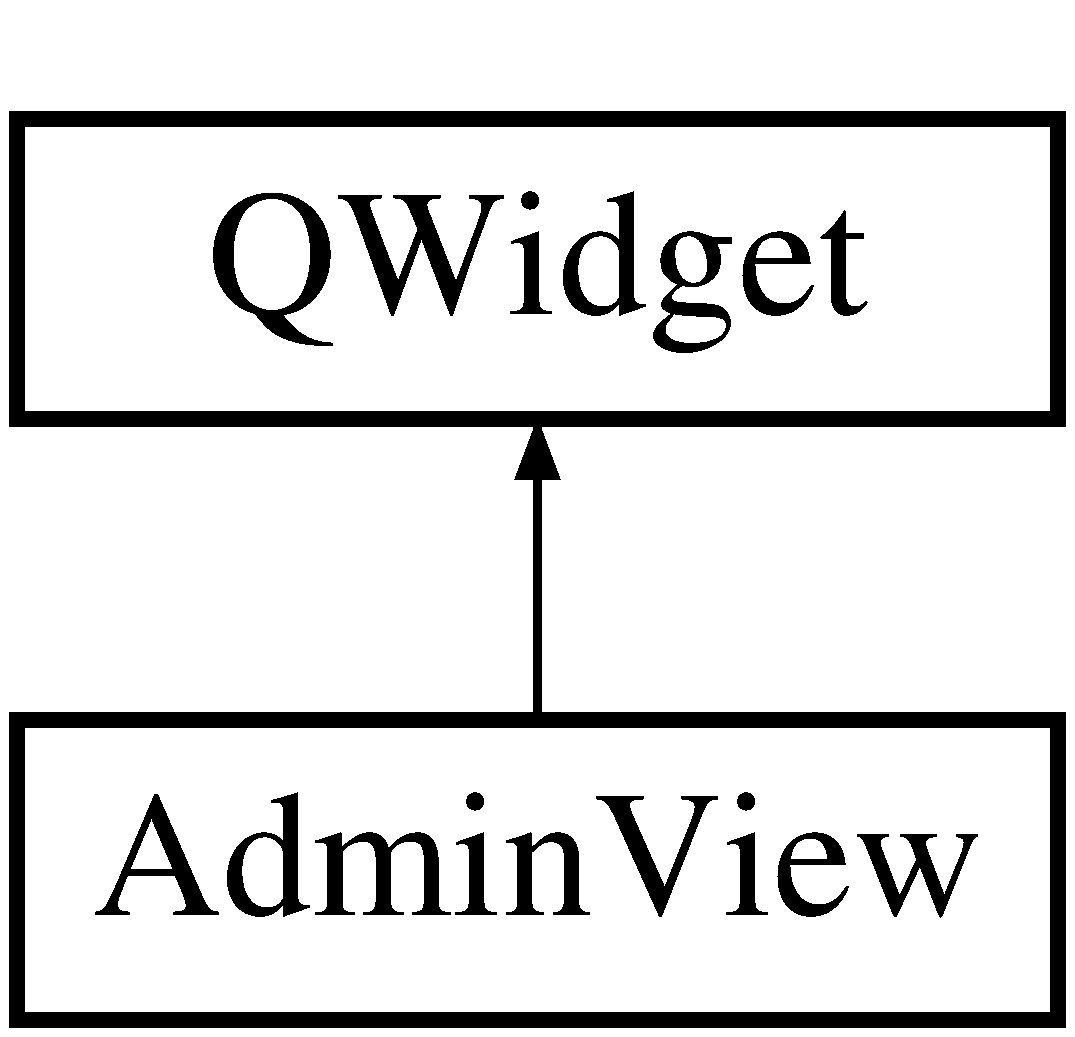
\includegraphics[height=2.000000cm]{classAdminView}
\end{center}
\end{figure}
\subsection*{Public Slots}
\begin{DoxyCompactItemize}
\item 
void \hyperlink{classAdminView_a0bc04afd4bcbf69f024599588b2caaaf}{reset\-View} ()
\begin{DoxyCompactList}\small\item\em Reset view as if it was just created. \end{DoxyCompactList}\item 
void \hyperlink{classAdminView_a383de7d879883a00b48eb32d614766de}{reset\-Ui} ()
\begin{DoxyCompactList}\small\item\em Reset lists, buttons, and fields to their original state. \end{DoxyCompactList}\end{DoxyCompactItemize}
\subsection*{Public Member Functions}
\begin{DoxyCompactItemize}
\item 
\hyperlink{classAdminView_a68e994ce28ee7af9fc8b0d87d5fb8edf}{Admin\-View} (Q\-Widget $\ast$parent, \hyperlink{classRestaurantDataStore}{Restaurant\-Data\-Store} $\ast$)
\begin{DoxyCompactList}\small\item\em Constructor. \end{DoxyCompactList}\item 
\hyperlink{classAdminView_acfefbeacc19672ae9bd0e365728c63ab}{$\sim$\-Admin\-View} () override
\begin{DoxyCompactList}\small\item\em Destructor. \end{DoxyCompactList}\end{DoxyCompactItemize}


\subsection{Detailed Description}
A view that handles tools for editing items of the given \hyperlink{classRestaurantDataStore}{Restaurant\-Data\-Store}. 

\subsection{Constructor \& Destructor Documentation}
\hypertarget{classAdminView_a68e994ce28ee7af9fc8b0d87d5fb8edf}{\index{Admin\-View@{Admin\-View}!Admin\-View@{Admin\-View}}
\index{Admin\-View@{Admin\-View}!AdminView@{Admin\-View}}
\subsubsection[{Admin\-View}]{\setlength{\rightskip}{0pt plus 5cm}Admin\-View\-::\-Admin\-View (
\begin{DoxyParamCaption}
\item[{Q\-Widget $\ast$}]{parent, }
\item[{{\bf Restaurant\-Data\-Store} $\ast$}]{data\-Store}
\end{DoxyParamCaption}
)}}\label{classAdminView_a68e994ce28ee7af9fc8b0d87d5fb8edf}


Constructor. 

Constructs a view for admin tools. Instantiates all the U\-I for the view and connects signals to slots.


\begin{DoxyParams}{Parameters}
{\em parent} & The parent widget this view will show up in \\
\hline
{\em data\-Store} & The datastore that this view can edit \\
\hline
\end{DoxyParams}
\hypertarget{classAdminView_acfefbeacc19672ae9bd0e365728c63ab}{\index{Admin\-View@{Admin\-View}!$\sim$\-Admin\-View@{$\sim$\-Admin\-View}}
\index{$\sim$\-Admin\-View@{$\sim$\-Admin\-View}!AdminView@{Admin\-View}}
\subsubsection[{$\sim$\-Admin\-View}]{\setlength{\rightskip}{0pt plus 5cm}Admin\-View\-::$\sim$\-Admin\-View (
\begin{DoxyParamCaption}
{}
\end{DoxyParamCaption}
)\hspace{0.3cm}{\ttfamily [override]}}}\label{classAdminView_acfefbeacc19672ae9bd0e365728c63ab}


Destructor. 

Delete dynamically allocated objects. 

\subsection{Member Function Documentation}
\hypertarget{classAdminView_a383de7d879883a00b48eb32d614766de}{\index{Admin\-View@{Admin\-View}!reset\-Ui@{reset\-Ui}}
\index{reset\-Ui@{reset\-Ui}!AdminView@{Admin\-View}}
\subsubsection[{reset\-Ui}]{\setlength{\rightskip}{0pt plus 5cm}void Admin\-View\-::reset\-Ui (
\begin{DoxyParamCaption}
{}
\end{DoxyParamCaption}
)\hspace{0.3cm}{\ttfamily [slot]}}}\label{classAdminView_a383de7d879883a00b48eb32d614766de}


Reset lists, buttons, and fields to their original state. 

Reload the restaurant lists. Reload the menu lists Redo push button stylesheets. Clear line edits. Set double spinboxes to zero. \hypertarget{classAdminView_a0bc04afd4bcbf69f024599588b2caaaf}{\index{Admin\-View@{Admin\-View}!reset\-View@{reset\-View}}
\index{reset\-View@{reset\-View}!AdminView@{Admin\-View}}
\subsubsection[{reset\-View}]{\setlength{\rightskip}{0pt plus 5cm}void Admin\-View\-::reset\-View (
\begin{DoxyParamCaption}
{}
\end{DoxyParamCaption}
)\hspace{0.3cm}{\ttfamily [slot]}}}\label{classAdminView_a0bc04afd4bcbf69f024599588b2caaaf}


Reset view as if it was just created. 

The current index of the stacked widget will be set to the first page (index 0). The current menu will be set to an invalid restaurant I\-D (-\/1). Reset the U\-I. 

The documentation for this class was generated from the following files\-:\begin{DoxyCompactItemize}
\item 
/home/edt/\-C\-S1\-D/\-C\-S1\-D\-\_\-\-Fast\-\_\-\-Food\-\_\-\-Project/\-Fast\-Food\-Finder/src/views/adminview.\-hpp\item 
/home/edt/\-C\-S1\-D/\-C\-S1\-D\-\_\-\-Fast\-\_\-\-Food\-\_\-\-Project/\-Fast\-Food\-Finder/src/views/adminview.\-cpp\end{DoxyCompactItemize}

\hypertarget{classBadFile}{\section{Bad\-File Class Reference}
\label{classBadFile}\index{Bad\-File@{Bad\-File}}
}
Inheritance diagram for Bad\-File\-:\begin{figure}[H]
\begin{center}
\leavevmode
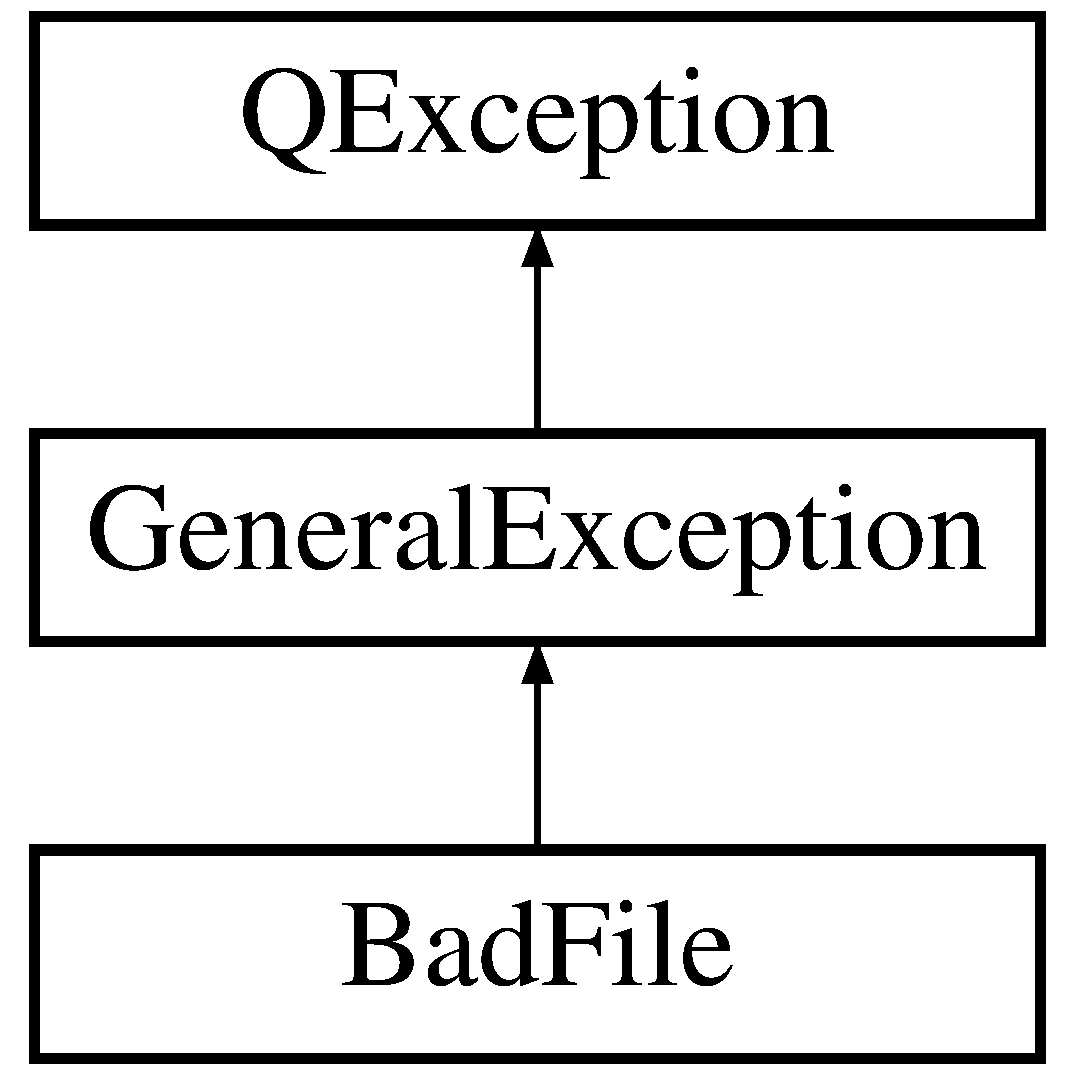
\includegraphics[height=3.000000cm]{classBadFile}
\end{center}
\end{figure}
\subsection*{Public Member Functions}
\begin{DoxyCompactItemize}
\item 
\hypertarget{classBadFile_aff3743219cfe8736a6a4f3630dc907d4}{{\bfseries Bad\-File} (Q\-String)}\label{classBadFile_aff3743219cfe8736a6a4f3630dc907d4}

\item 
\hypertarget{classBadFile_a3fd774c16c5808839343b60cf8d03a8b}{{\bfseries Bad\-File} (const Q\-File \&)}\label{classBadFile_a3fd774c16c5808839343b60cf8d03a8b}

\end{DoxyCompactItemize}
\subsection*{Additional Inherited Members}


The documentation for this class was generated from the following files\-:\begin{DoxyCompactItemize}
\item 
/home/edt/\-C\-S1\-D/\-C\-S1\-D\-\_\-\-Fast\-\_\-\-Food\-\_\-\-Project/\-Fast\-Food\-Finder/src/utils/exceptions.\-hpp\item 
/home/edt/\-C\-S1\-D/\-C\-S1\-D\-\_\-\-Fast\-\_\-\-Food\-\_\-\-Project/\-Fast\-Food\-Finder/src/utils/exceptions.\-cpp\end{DoxyCompactItemize}

\hypertarget{classBadFileFormat}{\section{Bad\-File\-Format Class Reference}
\label{classBadFileFormat}\index{Bad\-File\-Format@{Bad\-File\-Format}}
}
Inheritance diagram for Bad\-File\-Format\-:\begin{figure}[H]
\begin{center}
\leavevmode
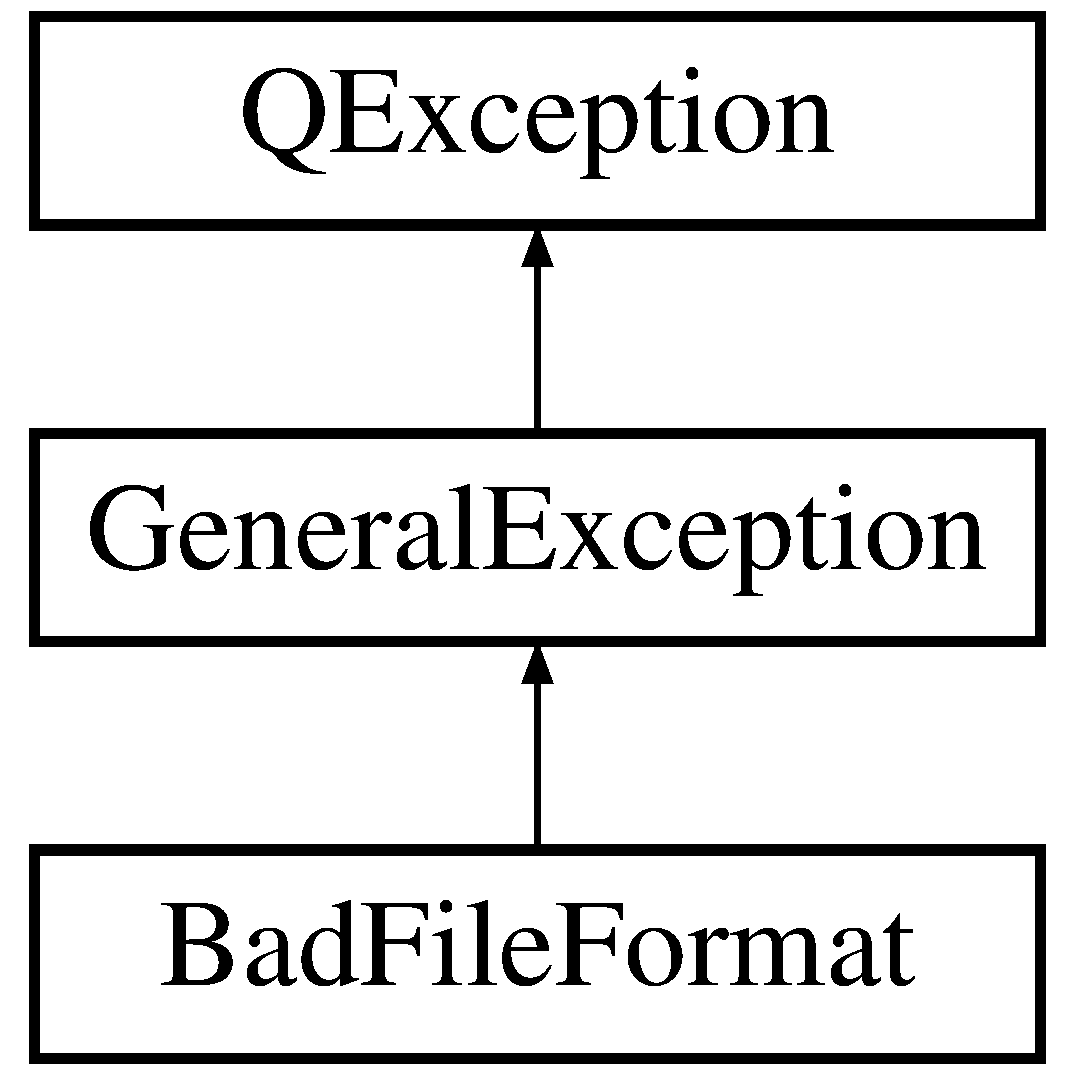
\includegraphics[height=3.000000cm]{classBadFileFormat}
\end{center}
\end{figure}
\subsection*{Public Member Functions}
\begin{DoxyCompactItemize}
\item 
\hypertarget{classBadFileFormat_af19928d559340e281b323edf230aa1bd}{{\bfseries Bad\-File\-Format} (Q\-String)}\label{classBadFileFormat_af19928d559340e281b323edf230aa1bd}

\item 
\hypertarget{classBadFileFormat_aee1f0e6299860c1ce8a04e65a149b42c}{{\bfseries Bad\-File\-Format} (Q\-String expected, Q\-String recieved)}\label{classBadFileFormat_aee1f0e6299860c1ce8a04e65a149b42c}

\end{DoxyCompactItemize}
\subsection*{Additional Inherited Members}


The documentation for this class was generated from the following files\-:\begin{DoxyCompactItemize}
\item 
/home/edt/\-C\-S1\-D/\-C\-S1\-D\-\_\-\-Fast\-\_\-\-Food\-\_\-\-Project/\-Fast\-Food\-Finder/src/utils/exceptions.\-hpp\item 
/home/edt/\-C\-S1\-D/\-C\-S1\-D\-\_\-\-Fast\-\_\-\-Food\-\_\-\-Project/\-Fast\-Food\-Finder/src/utils/exceptions.\-cpp\end{DoxyCompactItemize}

\hypertarget{structCmp__by__distance}{\section{Cmp\-\_\-by\-\_\-distance Struct Reference}
\label{structCmp__by__distance}\index{Cmp\-\_\-by\-\_\-distance@{Cmp\-\_\-by\-\_\-distance}}
}
\subsection*{Public Member Functions}
\begin{DoxyCompactItemize}
\item 
\hypertarget{structCmp__by__distance_a87a670a5b4dd789722149165c8fe7dfa}{bool {\bfseries operator()} (const \hyperlink{classRestaurant}{Restaurant} $\ast$s1, const \hyperlink{classRestaurant}{Restaurant} $\ast$s2) const }\label{structCmp__by__distance_a87a670a5b4dd789722149165c8fe7dfa}

\end{DoxyCompactItemize}


The documentation for this struct was generated from the following file\-:\begin{DoxyCompactItemize}
\item 
/home/edt/\-C\-S1\-D/\-C\-S1\-D\-\_\-\-Fast\-\_\-\-Food\-\_\-\-Project/\-Fast\-Food\-Finder/src/datastore/Restaurant.\-hpp\end{DoxyCompactItemize}

\hypertarget{structCmp__by__name}{\section{Cmp\-\_\-by\-\_\-name Struct Reference}
\label{structCmp__by__name}\index{Cmp\-\_\-by\-\_\-name@{Cmp\-\_\-by\-\_\-name}}
}
\subsection*{Public Member Functions}
\begin{DoxyCompactItemize}
\item 
\hypertarget{structCmp__by__name_a9118a502954850a1b036327f5e4d6b89}{bool {\bfseries operator()} (const \hyperlink{classRestaurant}{Restaurant} $\ast$s1, const \hyperlink{classRestaurant}{Restaurant} $\ast$s2) const }\label{structCmp__by__name_a9118a502954850a1b036327f5e4d6b89}

\end{DoxyCompactItemize}


The documentation for this struct was generated from the following file\-:\begin{DoxyCompactItemize}
\item 
/home/edt/\-C\-S1\-D/\-C\-S1\-D\-\_\-\-Fast\-\_\-\-Food\-\_\-\-Project/\-Fast\-Food\-Finder/src/datastore/Restaurant.\-hpp\end{DoxyCompactItemize}

\hypertarget{classnsMyDblLinkList_1_1MyDblLinkList_1_1const__iterator}{\section{ns\-My\-Dbl\-Link\-List\-:\-:My\-Dbl\-Link\-List$<$ Elem $>$\-:\-:const\-\_\-iterator Class Reference}
\label{classnsMyDblLinkList_1_1MyDblLinkList_1_1const__iterator}\index{ns\-My\-Dbl\-Link\-List\-::\-My\-Dbl\-Link\-List$<$ Elem $>$\-::const\-\_\-iterator@{ns\-My\-Dbl\-Link\-List\-::\-My\-Dbl\-Link\-List$<$ Elem $>$\-::const\-\_\-iterator}}
}
\subsection*{Public Member Functions}
\begin{DoxyCompactItemize}
\item 
\hypertarget{classnsMyDblLinkList_1_1MyDblLinkList_1_1const__iterator_a9e008134378bcae5c1c16d14a9467089}{{\bfseries const\-\_\-iterator} (\hyperlink{structnsMyDblLinkList_1_1Node}{Node}$<$ Elem $>$ $\ast$p)}\label{classnsMyDblLinkList_1_1MyDblLinkList_1_1const__iterator_a9e008134378bcae5c1c16d14a9467089}

\item 
\hypertarget{classnsMyDblLinkList_1_1MyDblLinkList_1_1const__iterator_a638bab6cee4e0c37567634cc3290706d}{\hyperlink{classnsMyDblLinkList_1_1MyDblLinkList_1_1iterator}{iterator} \& {\bfseries operator++} ()}\label{classnsMyDblLinkList_1_1MyDblLinkList_1_1const__iterator_a638bab6cee4e0c37567634cc3290706d}

\item 
\hypertarget{classnsMyDblLinkList_1_1MyDblLinkList_1_1const__iterator_a1fe3a2d04052d69245bb42b33d9c60d1}{\hyperlink{classnsMyDblLinkList_1_1MyDblLinkList_1_1const__iterator}{const\-\_\-iterator} \& {\bfseries operator-\/-\/} ()}\label{classnsMyDblLinkList_1_1MyDblLinkList_1_1const__iterator_a1fe3a2d04052d69245bb42b33d9c60d1}

\item 
\hypertarget{classnsMyDblLinkList_1_1MyDblLinkList_1_1const__iterator_ad2e81f125a9ed02ba82c496f0224e89f}{const Elem \& {\bfseries operator$\ast$} ()}\label{classnsMyDblLinkList_1_1MyDblLinkList_1_1const__iterator_ad2e81f125a9ed02ba82c496f0224e89f}

\item 
\hypertarget{classnsMyDblLinkList_1_1MyDblLinkList_1_1const__iterator_a22f2620df51d583f0a4f32b9c7bfea9b}{bool {\bfseries operator==} (const \hyperlink{classnsMyDblLinkList_1_1MyDblLinkList_1_1iterator}{iterator} \&rhs) const }\label{classnsMyDblLinkList_1_1MyDblLinkList_1_1const__iterator_a22f2620df51d583f0a4f32b9c7bfea9b}

\item 
\hypertarget{classnsMyDblLinkList_1_1MyDblLinkList_1_1const__iterator_a944ed6de382a995375e403e8f018608f}{bool {\bfseries operator!=} (const \hyperlink{classnsMyDblLinkList_1_1MyDblLinkList_1_1iterator}{iterator} \&rhs) const }\label{classnsMyDblLinkList_1_1MyDblLinkList_1_1const__iterator_a944ed6de382a995375e403e8f018608f}

\end{DoxyCompactItemize}


The documentation for this class was generated from the following file\-:\begin{DoxyCompactItemize}
\item 
/home/edt/\-C\-S1\-D/\-C\-S1\-D\-\_\-\-Fast\-\_\-\-Food\-\_\-\-Project/\-Fast\-Food\-Finder/src/datastore/My\-Dbl\-Link\-List.\-hpp\end{DoxyCompactItemize}

\hypertarget{classGeneralException}{\section{General\-Exception Class Reference}
\label{classGeneralException}\index{General\-Exception@{General\-Exception}}
}
Inheritance diagram for General\-Exception\-:\begin{figure}[H]
\begin{center}
\leavevmode
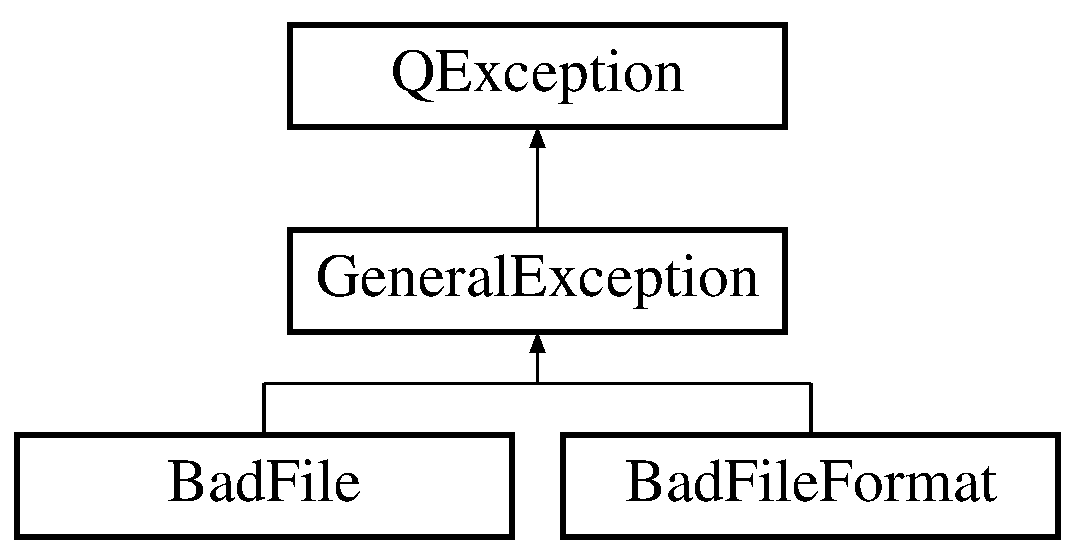
\includegraphics[height=3.000000cm]{classGeneralException}
\end{center}
\end{figure}
\subsection*{Public Member Functions}
\begin{DoxyCompactItemize}
\item 
\hypertarget{classGeneralException_a7185932f70f1e7cae580747ebb51c241}{{\bfseries General\-Exception} (Q\-String)}\label{classGeneralException_a7185932f70f1e7cae580747ebb51c241}

\item 
\hypertarget{classGeneralException_a5facd2adb3adc03412e419d9e2765cb7}{void {\bfseries error\-Window} () const }\label{classGeneralException_a5facd2adb3adc03412e419d9e2765cb7}

\item 
\hypertarget{classGeneralException_a175f8aa9d4f222fead2fe1b7e39f0835}{Q\-String {\bfseries error\-Message} () const }\label{classGeneralException_a175f8aa9d4f222fead2fe1b7e39f0835}

\item 
\hypertarget{classGeneralException_af8601a8d992b3d3b41675d428ac13eaa}{void {\bfseries raise} () const override}\label{classGeneralException_af8601a8d992b3d3b41675d428ac13eaa}

\item 
\hypertarget{classGeneralException_a328d69ca63d187ba0ae4d07f493e47c4}{\hyperlink{classGeneralException}{General\-Exception} $\ast$ {\bfseries clone} () const override}\label{classGeneralException_a328d69ca63d187ba0ae4d07f493e47c4}

\end{DoxyCompactItemize}
\subsection*{Protected Attributes}
\begin{DoxyCompactItemize}
\item 
\hypertarget{classGeneralException_af3e4ac87c597353172d3c5ec621f4925}{Q\-String {\bfseries message}}\label{classGeneralException_af3e4ac87c597353172d3c5ec621f4925}

\end{DoxyCompactItemize}


The documentation for this class was generated from the following files\-:\begin{DoxyCompactItemize}
\item 
/home/edt/\-C\-S1\-D/\-C\-S1\-D\-\_\-\-Fast\-\_\-\-Food\-\_\-\-Project/\-Fast\-Food\-Finder/src/utils/exceptions.\-hpp\item 
/home/edt/\-C\-S1\-D/\-C\-S1\-D\-\_\-\-Fast\-\_\-\-Food\-\_\-\-Project/\-Fast\-Food\-Finder/src/utils/exceptions.\-cpp\end{DoxyCompactItemize}

\hypertarget{classnsMyDblLinkList_1_1MyDblLinkList_1_1iterator}{\section{ns\-My\-Dbl\-Link\-List\-:\-:My\-Dbl\-Link\-List$<$ Elem $>$\-:\-:iterator Class Reference}
\label{classnsMyDblLinkList_1_1MyDblLinkList_1_1iterator}\index{ns\-My\-Dbl\-Link\-List\-::\-My\-Dbl\-Link\-List$<$ Elem $>$\-::iterator@{ns\-My\-Dbl\-Link\-List\-::\-My\-Dbl\-Link\-List$<$ Elem $>$\-::iterator}}
}
\subsection*{Public Member Functions}
\begin{DoxyCompactItemize}
\item 
\hypertarget{classnsMyDblLinkList_1_1MyDblLinkList_1_1iterator_a0a03daec3feadac5e779fa19eb0043bf}{{\bfseries iterator} (\hyperlink{structnsMyDblLinkList_1_1Node}{Node}$<$ Elem $>$ $\ast$p)}\label{classnsMyDblLinkList_1_1MyDblLinkList_1_1iterator_a0a03daec3feadac5e779fa19eb0043bf}

\item 
\hypertarget{classnsMyDblLinkList_1_1MyDblLinkList_1_1iterator_a0fe70fac59d4d62c80babea825f941a4}{\hyperlink{classnsMyDblLinkList_1_1MyDblLinkList_1_1iterator}{iterator} \& {\bfseries operator++} ()}\label{classnsMyDblLinkList_1_1MyDblLinkList_1_1iterator_a0fe70fac59d4d62c80babea825f941a4}

\item 
\hypertarget{classnsMyDblLinkList_1_1MyDblLinkList_1_1iterator_aa45611fe3370cc1fc305a75d1a2beb82}{\hyperlink{classnsMyDblLinkList_1_1MyDblLinkList_1_1iterator}{iterator} \& {\bfseries operator-\/-\/} ()}\label{classnsMyDblLinkList_1_1MyDblLinkList_1_1iterator_aa45611fe3370cc1fc305a75d1a2beb82}

\item 
\hypertarget{classnsMyDblLinkList_1_1MyDblLinkList_1_1iterator_ac13d5aaccc691771acc6fa716ef9c838}{\hyperlink{classnsMyDblLinkList_1_1MyDblLinkList_1_1iterator}{iterator} {\bfseries operator++} (int)}\label{classnsMyDblLinkList_1_1MyDblLinkList_1_1iterator_ac13d5aaccc691771acc6fa716ef9c838}

\item 
\hypertarget{classnsMyDblLinkList_1_1MyDblLinkList_1_1iterator_ae6d5f2d24ce61de8d55264bae3a90354}{Elem \& {\bfseries operator$\ast$} ()}\label{classnsMyDblLinkList_1_1MyDblLinkList_1_1iterator_ae6d5f2d24ce61de8d55264bae3a90354}

\item 
\hypertarget{classnsMyDblLinkList_1_1MyDblLinkList_1_1iterator_aad5a50af3aa3a4eae80032c22c98d132}{bool {\bfseries operator==} (const \hyperlink{classnsMyDblLinkList_1_1MyDblLinkList_1_1iterator}{iterator} \&rhs) const }\label{classnsMyDblLinkList_1_1MyDblLinkList_1_1iterator_aad5a50af3aa3a4eae80032c22c98d132}

\item 
\hypertarget{classnsMyDblLinkList_1_1MyDblLinkList_1_1iterator_a9c00af89376665439bc6aba958f10b11}{bool {\bfseries operator!=} (const \hyperlink{classnsMyDblLinkList_1_1MyDblLinkList_1_1iterator}{iterator} \&rhs) const }\label{classnsMyDblLinkList_1_1MyDblLinkList_1_1iterator_a9c00af89376665439bc6aba958f10b11}

\end{DoxyCompactItemize}


The documentation for this class was generated from the following file\-:\begin{DoxyCompactItemize}
\item 
/home/edt/\-C\-S1\-D/\-C\-S1\-D\-\_\-\-Fast\-\_\-\-Food\-\_\-\-Project/\-Fast\-Food\-Finder/src/datastore/My\-Dbl\-Link\-List.\-hpp\end{DoxyCompactItemize}

\hypertarget{classLogin}{\section{Login Class Reference}
\label{classLogin}\index{Login@{Login}}
}


\hyperlink{classLogin}{Login} class.  




{\ttfamily \#include $<$login.\-hpp$>$}

Inheritance diagram for Login\-:\begin{figure}[H]
\begin{center}
\leavevmode
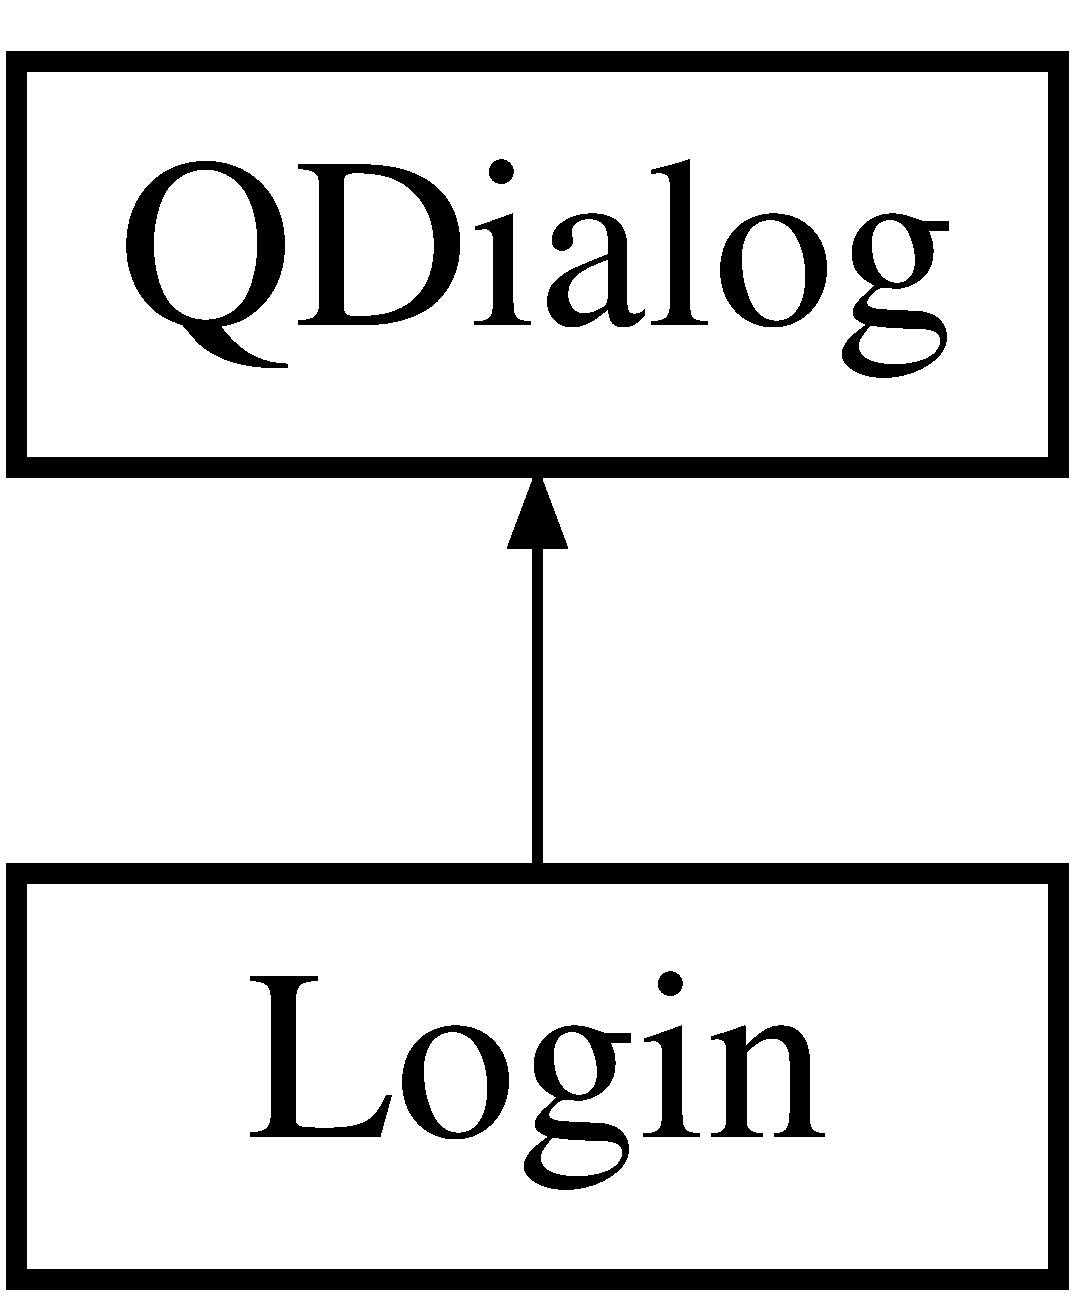
\includegraphics[height=2.000000cm]{classLogin}
\end{center}
\end{figure}
\subsection*{Public Types}
\begin{DoxyCompactItemize}
\item 
enum {\bfseries Type} \{ {\bfseries U\-S\-E\-R}, 
{\bfseries A\-D\-M\-I\-N}
 \}
\end{DoxyCompactItemize}
\subsection*{Static Public Member Functions}
\begin{DoxyCompactItemize}
\item 
static \hyperlink{classLogin}{Login} $\ast$ \hyperlink{classLogin_a369d9ce9b0debac51fb72a234fd82b03}{get\-Instance} ()
\begin{DoxyCompactList}\small\item\em Getter. \end{DoxyCompactList}\item 
static Type \hyperlink{classLogin_ab23eec7779982cad2ceac3d25ac4aa26}{get\-Type} ()
\begin{DoxyCompactList}\small\item\em Getter. \end{DoxyCompactList}\item 
static void \hyperlink{classLogin_a82b6030d49444a1b60a375983b1798ca}{request\-Login} ()
\begin{DoxyCompactList}\small\item\em \hyperlink{classLogin}{Login} usage. \end{DoxyCompactList}\end{DoxyCompactItemize}


\subsection{Detailed Description}
\hyperlink{classLogin}{Login} class. 

Provides a simple way to request a login in order to validate a user.

To use\-: 
\begin{DoxyCode}
QObject::connect(\hyperlink{classLogin_a369d9ce9b0debac51fb72a234fd82b03}{Login::getInstance}(), &Login::accepted,
                 myWidgetPointer, &MyClass::mySlot);
\end{DoxyCode}


This will call \&My\-Class\-::my\-Slot upon my\-Widget\-Pointer when login is accepted. 

\subsection{Member Function Documentation}
\hypertarget{classLogin_a369d9ce9b0debac51fb72a234fd82b03}{\index{Login@{Login}!get\-Instance@{get\-Instance}}
\index{get\-Instance@{get\-Instance}!Login@{Login}}
\subsubsection[{get\-Instance}]{\setlength{\rightskip}{0pt plus 5cm}{\bf Login} $\ast$ Login\-::get\-Instance (
\begin{DoxyParamCaption}
{}
\end{DoxyParamCaption}
)\hspace{0.3cm}{\ttfamily [static]}}}\label{classLogin_a369d9ce9b0debac51fb72a234fd82b03}


Getter. 

If there isn't a current instance, one will be created as well as the credential file.

\begin{DoxyReturn}{Returns}
Singleton instance 
\end{DoxyReturn}
\hypertarget{classLogin_ab23eec7779982cad2ceac3d25ac4aa26}{\index{Login@{Login}!get\-Type@{get\-Type}}
\index{get\-Type@{get\-Type}!Login@{Login}}
\subsubsection[{get\-Type}]{\setlength{\rightskip}{0pt plus 5cm}Login\-::\-Type Login\-::get\-Type (
\begin{DoxyParamCaption}
{}
\end{DoxyParamCaption}
)\hspace{0.3cm}{\ttfamily [static]}}}\label{classLogin_ab23eec7779982cad2ceac3d25ac4aa26}


Getter. 

Returns the login type of the last user that logged in

\begin{DoxyReturn}{Returns}
\hyperlink{classLogin}{Login} type of the last user that logged in 
\end{DoxyReturn}
\hypertarget{classLogin_a82b6030d49444a1b60a375983b1798ca}{\index{Login@{Login}!request\-Login@{request\-Login}}
\index{request\-Login@{request\-Login}!Login@{Login}}
\subsubsection[{request\-Login}]{\setlength{\rightskip}{0pt plus 5cm}void Login\-::request\-Login (
\begin{DoxyParamCaption}
{}
\end{DoxyParamCaption}
)\hspace{0.3cm}{\ttfamily [static]}}}\label{classLogin_a82b6030d49444a1b60a375983b1798ca}


\hyperlink{classLogin}{Login} usage. 

Requests a login screen. Calls \hyperlink{classLogin_a369d9ce9b0debac51fb72a234fd82b03}{get\-Instance()} in case it hasn't been called yet. 

The documentation for this class was generated from the following files\-:\begin{DoxyCompactItemize}
\item 
/home/edt/\-C\-S1\-D/\-C\-S1\-D\-\_\-\-Fast\-\_\-\-Food\-\_\-\-Project/\-Fast\-Food\-Finder/src/windows/login.\-hpp\item 
/home/edt/\-C\-S1\-D/\-C\-S1\-D\-\_\-\-Fast\-\_\-\-Food\-\_\-\-Project/\-Fast\-Food\-Finder/src/windows/login.\-cpp\end{DoxyCompactItemize}

\hypertarget{classMainWindow}{\section{Main\-Window Class Reference}
\label{classMainWindow}\index{Main\-Window@{Main\-Window}}
}
Inheritance diagram for Main\-Window\-:\begin{figure}[H]
\begin{center}
\leavevmode
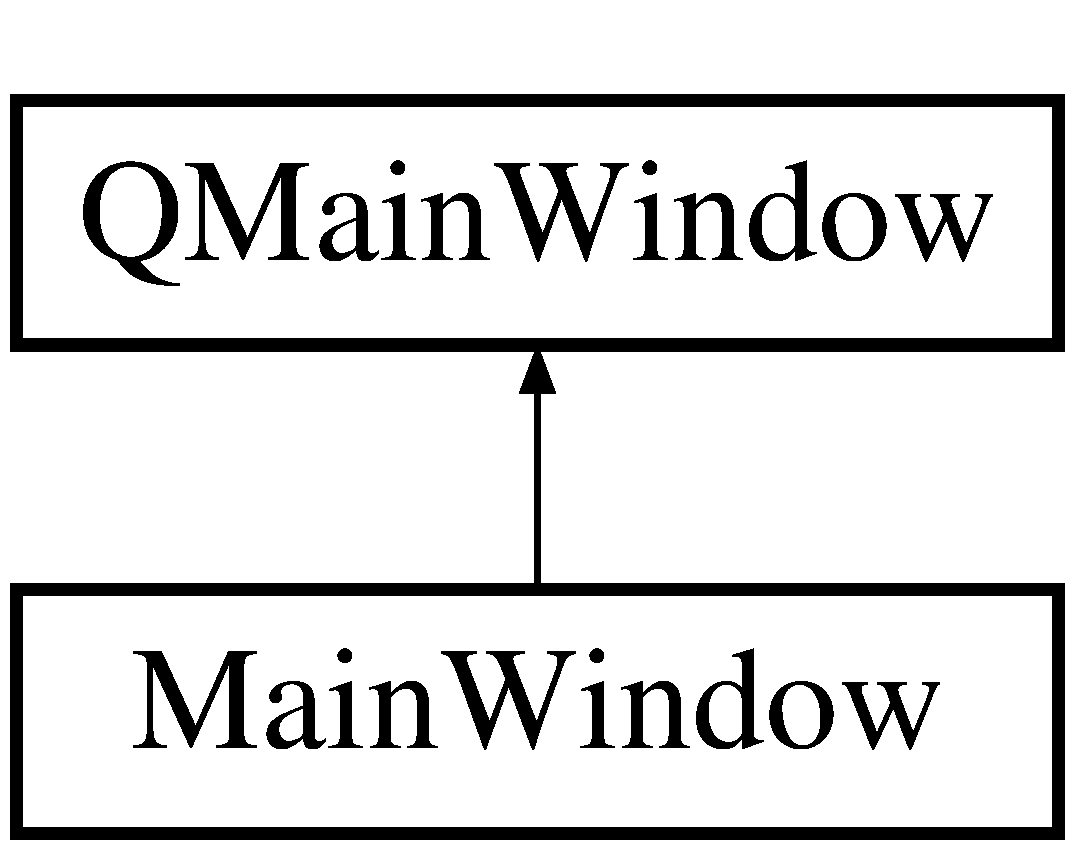
\includegraphics[height=2.000000cm]{classMainWindow}
\end{center}
\end{figure}
\subsection*{Signals}
\begin{DoxyCompactItemize}
\item 
\hypertarget{classMainWindow_a5ece302f5e733ada9b8f1a53a7f7a643}{void {\bfseries logout} () const }\label{classMainWindow_a5ece302f5e733ada9b8f1a53a7f7a643}

\end{DoxyCompactItemize}


The documentation for this class was generated from the following files\-:\begin{DoxyCompactItemize}
\item 
/home/edt/\-C\-S1\-D/\-C\-S1\-D\-\_\-\-Fast\-\_\-\-Food\-\_\-\-Project/\-Fast\-Food\-Finder/src/windows/mainwindow.\-hpp\item 
/home/edt/\-C\-S1\-D/\-C\-S1\-D\-\_\-\-Fast\-\_\-\-Food\-\_\-\-Project/\-Fast\-Food\-Finder/src/windows/mainwindow.\-cpp\end{DoxyCompactItemize}

\hypertarget{classMenuItem}{\section{Menu\-Item Class Reference}
\label{classMenuItem}\index{Menu\-Item@{Menu\-Item}}
}


{\ttfamily \#include $<$Menu\-Item.\-hpp$>$}

\subsection*{Public Member Functions}
\begin{DoxyCompactItemize}
\item 
virtual \hyperlink{classMenuItem_a41c6086a4d066256ecb7bfa715059ea2}{$\sim$\-Menu\-Item} ()
\item 
\hyperlink{classMenuItem_a502e53d939dcf20757666b059cba9664}{Menu\-Item} (const \hyperlink{classMenuItem}{Menu\-Item} \&src)
\item 
\hyperlink{classMenuItem}{Menu\-Item} \& \hyperlink{classMenuItem_a68edba703c28553a8d929407ddce5d94}{operator=} (const \hyperlink{classMenuItem}{Menu\-Item} \&rhs)
\item 
int \hyperlink{classMenuItem_aac2b3c2395c2e4e6126a885c9613afba}{Get\-Number} (void) const 
\item 
float \hyperlink{classMenuItem_a1079d7b1a336e62a02e7fcdbcf0adfa7}{Get\-Price} (void) const 
\item 
void \hyperlink{classMenuItem_a434d85549390ce6fd10c370403607812}{Update\-Price} (const float New\-Price)
\item 
const string \& \hyperlink{classMenuItem_afb088804ca10808f8039303814e8ac59}{Get\-Name} (void) const 
\item 
void \hyperlink{classMenuItem_a9657a4b4274f27e5210524ebfd724248}{Update\-Name} (const string \&New\-Name)
\item 
bool \hyperlink{classMenuItem_a53b89f5c25bba630a2ab169f3c6b4f3c}{Is\-Deleted} (void) const 
\item 
bool \hyperlink{classMenuItem_aeef040758879fcf8509c277fb88ceb4d}{Mark\-Deleted} (bool Delete)
\item 
\hypertarget{classMenuItem_a4738e0e464e49c9e4515305d6caa0075}{const \hyperlink{classMenuItem}{Menu\-Item} \& {\bfseries Find\-Menu\-Itemby\-Number} (int Number) const }\label{classMenuItem_a4738e0e464e49c9e4515305d6caa0075}

\end{DoxyCompactItemize}
\subsection*{Friends}
\begin{DoxyCompactItemize}
\item 
\hypertarget{classMenuItem_afa3daf805a237e2dca6b6e781e84bfb8}{class {\bfseries Restaurant}}\label{classMenuItem_afa3daf805a237e2dca6b6e781e84bfb8}

\item 
\hypertarget{classMenuItem_af6d4a4f1eb97251a24add34c6978faa2}{class {\bfseries Restaurant\-Data\-Store}}\label{classMenuItem_af6d4a4f1eb97251a24add34c6978faa2}

\end{DoxyCompactItemize}


\subsection{Detailed Description}
\hyperlink{classMenuItem}{Menu\-Item} Class

\begin{DoxyAuthor}{Author}
edt (3/25/19) 
\end{DoxyAuthor}


\subsection{Constructor \& Destructor Documentation}
\hypertarget{classMenuItem_a41c6086a4d066256ecb7bfa715059ea2}{\index{Menu\-Item@{Menu\-Item}!$\sim$\-Menu\-Item@{$\sim$\-Menu\-Item}}
\index{$\sim$\-Menu\-Item@{$\sim$\-Menu\-Item}!MenuItem@{Menu\-Item}}
\subsubsection[{$\sim$\-Menu\-Item}]{\setlength{\rightskip}{0pt plus 5cm}Menu\-Item\-::$\sim$\-Menu\-Item (
\begin{DoxyParamCaption}
{}
\end{DoxyParamCaption}
)\hspace{0.3cm}{\ttfamily [virtual]}}}\label{classMenuItem_a41c6086a4d066256ecb7bfa715059ea2}
C\-S1\-D -\/ Fast Food Associates

Implemention of the Meni\-Item class that provides a means for validating menu items, string menu items and prices

\begin{DoxyAuthor}{Author}
edt\-Menu\-Item default constructor

edt (3/25/19) 
\end{DoxyAuthor}
\hypertarget{classMenuItem_a502e53d939dcf20757666b059cba9664}{\index{Menu\-Item@{Menu\-Item}!Menu\-Item@{Menu\-Item}}
\index{Menu\-Item@{Menu\-Item}!MenuItem@{Menu\-Item}}
\subsubsection[{Menu\-Item}]{\setlength{\rightskip}{0pt plus 5cm}Menu\-Item\-::\-Menu\-Item (
\begin{DoxyParamCaption}
\item[{const {\bf Menu\-Item} \&}]{src}
\end{DoxyParamCaption}
)}}\label{classMenuItem_a502e53d939dcf20757666b059cba9664}
\hyperlink{classMenuItem_a502e53d939dcf20757666b059cba9664}{Menu\-Item\-::\-Menu\-Item} -\/ copy constructor

\begin{DoxyAuthor}{Author}
edt (3/25/19)
\end{DoxyAuthor}

\begin{DoxyParams}{Parameters}
{\em src} & -\/ item to copy \\
\hline
\end{DoxyParams}


\subsection{Member Function Documentation}
\hypertarget{classMenuItem_afb088804ca10808f8039303814e8ac59}{\index{Menu\-Item@{Menu\-Item}!Get\-Name@{Get\-Name}}
\index{Get\-Name@{Get\-Name}!MenuItem@{Menu\-Item}}
\subsubsection[{Get\-Name}]{\setlength{\rightskip}{0pt plus 5cm}const string \& Menu\-Item\-::\-Get\-Name (
\begin{DoxyParamCaption}
\item[{void}]{}
\end{DoxyParamCaption}
) const}}\label{classMenuItem_afb088804ca10808f8039303814e8ac59}
\hyperlink{classMenuItem_afb088804ca10808f8039303814e8ac59}{Menu\-Item\-::\-Get\-Name}

\begin{DoxyAuthor}{Author}
edt (3/25/19)
\end{DoxyAuthor}

\begin{DoxyParams}{Parameters}
{\em void} & \\
\hline
\end{DoxyParams}
\begin{DoxyReturn}{Returns}
const string\& Name of Item 
\end{DoxyReturn}
\hypertarget{classMenuItem_aac2b3c2395c2e4e6126a885c9613afba}{\index{Menu\-Item@{Menu\-Item}!Get\-Number@{Get\-Number}}
\index{Get\-Number@{Get\-Number}!MenuItem@{Menu\-Item}}
\subsubsection[{Get\-Number}]{\setlength{\rightskip}{0pt plus 5cm}int Menu\-Item\-::\-Get\-Number (
\begin{DoxyParamCaption}
\item[{void}]{}
\end{DoxyParamCaption}
) const}}\label{classMenuItem_aac2b3c2395c2e4e6126a885c9613afba}
\hyperlink{classMenuItem_aac2b3c2395c2e4e6126a885c9613afba}{Menu\-Item\-::\-Get\-Number}

\begin{DoxyAuthor}{Author}
edt (3/25/19)
\end{DoxyAuthor}

\begin{DoxyParams}{Parameters}
{\em void} & \\
\hline
\end{DoxyParams}
\begin{DoxyReturn}{Returns}
int -\/ number of this item 
\end{DoxyReturn}
\hypertarget{classMenuItem_a1079d7b1a336e62a02e7fcdbcf0adfa7}{\index{Menu\-Item@{Menu\-Item}!Get\-Price@{Get\-Price}}
\index{Get\-Price@{Get\-Price}!MenuItem@{Menu\-Item}}
\subsubsection[{Get\-Price}]{\setlength{\rightskip}{0pt plus 5cm}float Menu\-Item\-::\-Get\-Price (
\begin{DoxyParamCaption}
\item[{void}]{}
\end{DoxyParamCaption}
) const}}\label{classMenuItem_a1079d7b1a336e62a02e7fcdbcf0adfa7}
\hyperlink{classMenuItem_a1079d7b1a336e62a02e7fcdbcf0adfa7}{Menu\-Item\-::\-Get\-Price}

\begin{DoxyAuthor}{Author}
edt (3/25/19)
\end{DoxyAuthor}

\begin{DoxyParams}{Parameters}
{\em void} & \\
\hline
\end{DoxyParams}
\begin{DoxyReturn}{Returns}
float -\/ price of item 
\end{DoxyReturn}
\hypertarget{classMenuItem_a53b89f5c25bba630a2ab169f3c6b4f3c}{\index{Menu\-Item@{Menu\-Item}!Is\-Deleted@{Is\-Deleted}}
\index{Is\-Deleted@{Is\-Deleted}!MenuItem@{Menu\-Item}}
\subsubsection[{Is\-Deleted}]{\setlength{\rightskip}{0pt plus 5cm}bool Menu\-Item\-::\-Is\-Deleted (
\begin{DoxyParamCaption}
\item[{void}]{}
\end{DoxyParamCaption}
) const}}\label{classMenuItem_a53b89f5c25bba630a2ab169f3c6b4f3c}
\hyperlink{classMenuItem_a53b89f5c25bba630a2ab169f3c6b4f3c}{Menu\-Item\-::\-Is\-Deleted}

\begin{DoxyAuthor}{Author}
edt (3/25/19)
\end{DoxyAuthor}

\begin{DoxyParams}{Parameters}
{\em void} & \\
\hline
\end{DoxyParams}
\begin{DoxyReturn}{Returns}
bool -\/ 
\end{DoxyReturn}
\hypertarget{classMenuItem_aeef040758879fcf8509c277fb88ceb4d}{\index{Menu\-Item@{Menu\-Item}!Mark\-Deleted@{Mark\-Deleted}}
\index{Mark\-Deleted@{Mark\-Deleted}!MenuItem@{Menu\-Item}}
\subsubsection[{Mark\-Deleted}]{\setlength{\rightskip}{0pt plus 5cm}bool Menu\-Item\-::\-Mark\-Deleted (
\begin{DoxyParamCaption}
\item[{bool}]{Delete}
\end{DoxyParamCaption}
)}}\label{classMenuItem_aeef040758879fcf8509c277fb88ceb4d}
\hyperlink{classMenuItem_aeef040758879fcf8509c277fb88ceb4d}{Menu\-Item\-::\-Mark\-Deleted}

\begin{DoxyAuthor}{Author}
edt (3/25/19)
\end{DoxyAuthor}

\begin{DoxyParams}{Parameters}
{\em Delete} & -\/ true to mark item deleted\\
\hline
\end{DoxyParams}
\begin{DoxyReturn}{Returns}
bool -\/ true if item is deleted and should not be used for new trips 
\end{DoxyReturn}
\hypertarget{classMenuItem_a68edba703c28553a8d929407ddce5d94}{\index{Menu\-Item@{Menu\-Item}!operator=@{operator=}}
\index{operator=@{operator=}!MenuItem@{Menu\-Item}}
\subsubsection[{operator=}]{\setlength{\rightskip}{0pt plus 5cm}{\bf Menu\-Item} \& Menu\-Item\-::operator= (
\begin{DoxyParamCaption}
\item[{const {\bf Menu\-Item} \&}]{rhs}
\end{DoxyParamCaption}
)}}\label{classMenuItem_a68edba703c28553a8d929407ddce5d94}
\hyperlink{classMenuItem_a68edba703c28553a8d929407ddce5d94}{Menu\-Item\-::operator=}

\begin{DoxyAuthor}{Author}
edt (3/25/19)
\end{DoxyAuthor}

\begin{DoxyParams}{Parameters}
{\em rhs} & -\/ item to copy\\
\hline
\end{DoxyParams}
\begin{DoxyReturn}{Returns}
\hyperlink{classMenuItem}{Menu\-Item}\& 
\end{DoxyReturn}
\hypertarget{classMenuItem_a9657a4b4274f27e5210524ebfd724248}{\index{Menu\-Item@{Menu\-Item}!Update\-Name@{Update\-Name}}
\index{Update\-Name@{Update\-Name}!MenuItem@{Menu\-Item}}
\subsubsection[{Update\-Name}]{\setlength{\rightskip}{0pt plus 5cm}void Menu\-Item\-::\-Update\-Name (
\begin{DoxyParamCaption}
\item[{const string \&}]{New\-Name}
\end{DoxyParamCaption}
)}}\label{classMenuItem_a9657a4b4274f27e5210524ebfd724248}
\hyperlink{classMenuItem_a9657a4b4274f27e5210524ebfd724248}{Menu\-Item\-::\-Update\-Name}

\begin{DoxyAuthor}{Author}
edt (3/25/19)
\end{DoxyAuthor}

\begin{DoxyParams}{Parameters}
{\em New\-Name} & -\/ new name for item \\
\hline
\end{DoxyParams}
\hypertarget{classMenuItem_a434d85549390ce6fd10c370403607812}{\index{Menu\-Item@{Menu\-Item}!Update\-Price@{Update\-Price}}
\index{Update\-Price@{Update\-Price}!MenuItem@{Menu\-Item}}
\subsubsection[{Update\-Price}]{\setlength{\rightskip}{0pt plus 5cm}void Menu\-Item\-::\-Update\-Price (
\begin{DoxyParamCaption}
\item[{const float}]{New\-Price}
\end{DoxyParamCaption}
)}}\label{classMenuItem_a434d85549390ce6fd10c370403607812}
\hyperlink{classMenuItem_a434d85549390ce6fd10c370403607812}{Menu\-Item\-::\-Update\-Price}

\begin{DoxyAuthor}{Author}
edt (3/25/19)
\end{DoxyAuthor}

\begin{DoxyParams}{Parameters}
{\em New\-Price} & -\/ updated orice of item \\
\hline
\end{DoxyParams}


The documentation for this class was generated from the following files\-:\begin{DoxyCompactItemize}
\item 
/home/edt/\-C\-S1\-D/\-C\-S1\-D\-\_\-\-Fast\-\_\-\-Food\-\_\-\-Project/\-Fast\-Food\-Finder/src/datastore/Menu\-Item.\-hpp\item 
/home/edt/\-C\-S1\-D/\-C\-S1\-D\-\_\-\-Fast\-\_\-\-Food\-\_\-\-Project/\-Fast\-Food\-Finder/src/datastore/Menu\-Item.\-cpp\end{DoxyCompactItemize}

\hypertarget{classMenuList}{\section{Menu\-List Class Reference}
\label{classMenuList}\index{Menu\-List@{Menu\-List}}
}


\hyperlink{classMenuList}{Menu\-List} class.  




{\ttfamily \#include $<$menulist.\-hpp$>$}

Inheritance diagram for Menu\-List\-:\begin{figure}[H]
\begin{center}
\leavevmode
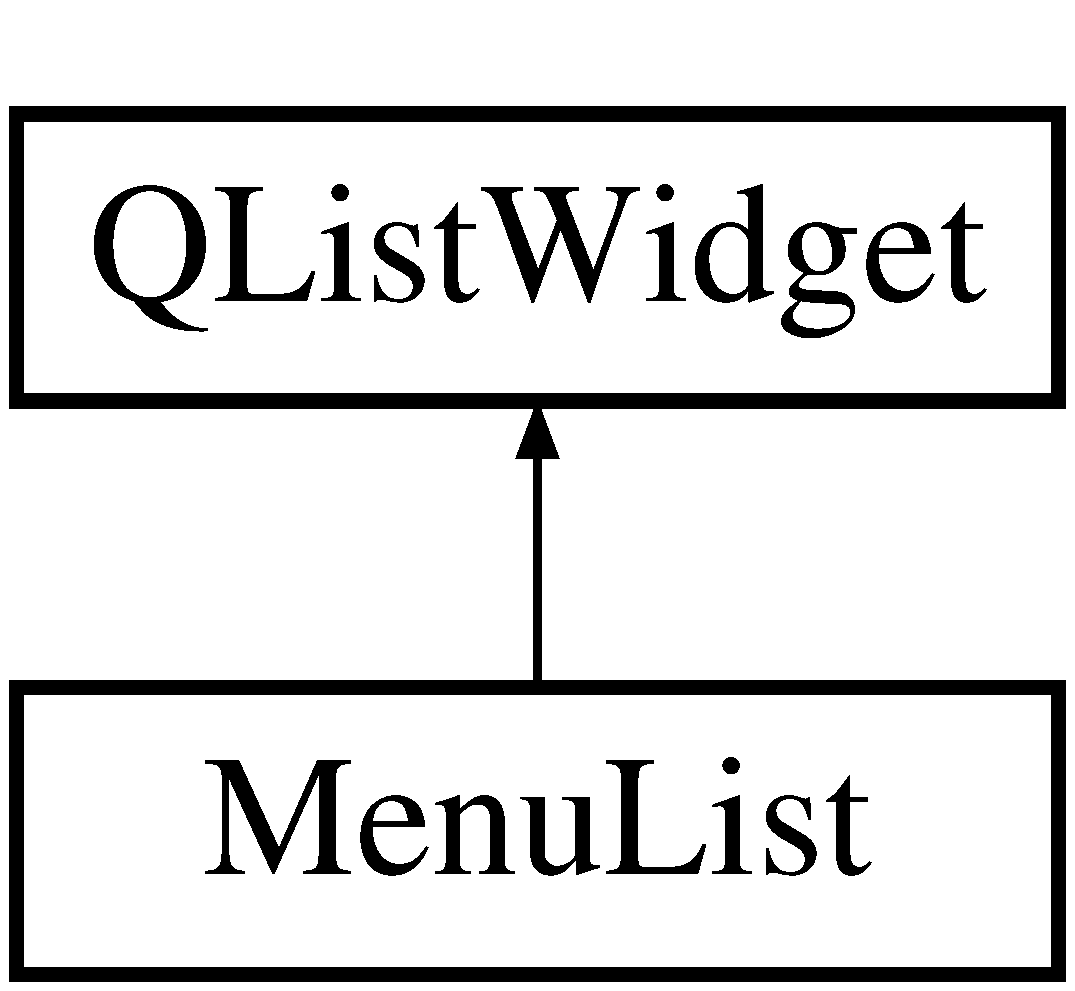
\includegraphics[height=2.000000cm]{classMenuList}
\end{center}
\end{figure}
\subsection*{Signals}
\begin{DoxyCompactItemize}
\item 
\hypertarget{classMenuList_a8eb7badea0b913bf4d3916d5b92c8f93}{void {\bfseries current\-Menu\-Item\-Changed} (I\-Ds) const }\label{classMenuList_a8eb7badea0b913bf4d3916d5b92c8f93}

\item 
\hypertarget{classMenuList_a3a1b1b0037c02a3a55a6870bd268aee6}{void {\bfseries show\-Qty\-Emitter} (bool) const }\label{classMenuList_a3a1b1b0037c02a3a55a6870bd268aee6}

\item 
\hypertarget{classMenuList_a7eb1c68ab9247e9c7c89d5a853193863}{void {\bfseries reset\-Qty\-Emitter} () const }\label{classMenuList_a7eb1c68ab9247e9c7c89d5a853193863}

\end{DoxyCompactItemize}
\subsection*{Public Member Functions}
\begin{DoxyCompactItemize}
\item 
\hyperlink{classMenuList_afb9e9b923adf9028f08077a37aeedf21}{Menu\-List} (Q\-Widget $\ast$parent)
\begin{DoxyCompactList}\small\item\em Constructor. \end{DoxyCompactList}\item 
I\-D\-Qtys \hyperlink{classMenuList_abfec38982e1bf286a6c703493f04905f}{get\-I\-D\-Qty} () const 
\begin{DoxyCompactList}\small\item\em Get I\-Ds and its corresponding spinbox value. \end{DoxyCompactList}\item 
I\-Ds \hyperlink{classMenuList_a42df740f9efcd34a13379681ad52c687}{get\-Selected} () const 
\begin{DoxyCompactList}\small\item\em Get selected I\-Ds. \end{DoxyCompactList}\item 
void \hyperlink{classMenuList_ab6ff6611ff4f26da63f424d78f455b81}{set\-Qty} (I\-Ds, int qty) const 
\begin{DoxyCompactList}\small\item\em Set I\-Ds' quantity. \end{DoxyCompactList}\item 
void \hyperlink{classMenuList_abe044f2d6c96e53cdedcdc01dcce2c6b}{add\-Item} (Restaurant\-I\-D, const \hyperlink{classMenuItem}{Menu\-Item} \&)
\begin{DoxyCompactList}\small\item\em Add menu item to the list. \end{DoxyCompactList}\item 
void \hyperlink{classMenuList_ad3fa59fa9c0f70232bc7b3d249ec880a}{add\-All\-Items} (const \hyperlink{classRestaurant}{Restaurant} \&)
\begin{DoxyCompactList}\small\item\em Add multiple menu items to the list. \end{DoxyCompactList}\item 
void \hyperlink{classMenuList_acb345e457dcbcb3078aa85bb604cc579}{remove\-Item} (I\-Ds)
\begin{DoxyCompactList}\small\item\em Remove menu item from the list. \end{DoxyCompactList}\item 
void \hyperlink{classMenuList_a8faf240cbb8449b2975fdb95dd2cbbe3}{show\-Hidden} (bool)
\begin{DoxyCompactList}\small\item\em Allow hidden menu items. \end{DoxyCompactList}\item 
void \hyperlink{classMenuList_a44b4b3bc30516463b8c17399e668144f}{show\-Qty} (bool)
\begin{DoxyCompactList}\small\item\em Show the quantity spinbox. \end{DoxyCompactList}\item 
void \hyperlink{classMenuList_abfedeff97ef2d0cc4505fe7c793d5c87}{reset\-Qty} ()
\begin{DoxyCompactList}\small\item\em Reset quantities. \end{DoxyCompactList}\end{DoxyCompactItemize}


\subsection{Detailed Description}
\hyperlink{classMenuList}{Menu\-List} class. 

Provides a simple way to list menu items. This list isn't tied to a specific restaurant, any menu item can be added.

To use\-: 
\begin{DoxyCode}
\hyperlink{classMenuList}{MenuList}* list = \textcolor{keyword}{new} \hyperlink{classRestaurantList}{RestaurantList}(widget);
list->\hyperlink{classMenuList_ad3fa59fa9c0f70232bc7b3d249ec880a}{addAllItems}(restaurant);
\end{DoxyCode}


This will create a menu list within its parent widget. Then it will add all the menu items of the restaurant to the list. 

\subsection{Constructor \& Destructor Documentation}
\hypertarget{classMenuList_afb9e9b923adf9028f08077a37aeedf21}{\index{Menu\-List@{Menu\-List}!Menu\-List@{Menu\-List}}
\index{Menu\-List@{Menu\-List}!MenuList@{Menu\-List}}
\subsubsection[{Menu\-List}]{\setlength{\rightskip}{0pt plus 5cm}Menu\-List\-::\-Menu\-List (
\begin{DoxyParamCaption}
\item[{Q\-Widget $\ast$}]{parent}
\end{DoxyParamCaption}
)}}\label{classMenuList_afb9e9b923adf9028f08077a37aeedf21}


Constructor. 

Constructs a menu list within the given parent widget. All default settings are set when created.


\begin{DoxyParams}{Parameters}
{\em parent} & The widget to display the list in \\
\hline
\end{DoxyParams}


\subsection{Member Function Documentation}
\hypertarget{classMenuList_ad3fa59fa9c0f70232bc7b3d249ec880a}{\index{Menu\-List@{Menu\-List}!add\-All\-Items@{add\-All\-Items}}
\index{add\-All\-Items@{add\-All\-Items}!MenuList@{Menu\-List}}
\subsubsection[{add\-All\-Items}]{\setlength{\rightskip}{0pt plus 5cm}void Menu\-List\-::add\-All\-Items (
\begin{DoxyParamCaption}
\item[{const {\bf Restaurant} \&}]{restaurant}
\end{DoxyParamCaption}
)}}\label{classMenuList_ad3fa59fa9c0f70232bc7b3d249ec880a}


Add multiple menu items to the list. 

Appends multiple menu items to the list given a restaurant. Calls \hyperlink{classMenuList_abe044f2d6c96e53cdedcdc01dcce2c6b}{Menu\-List\-::add\-Item()} for each menu item of the restaurant.


\begin{DoxyParams}{Parameters}
{\em restaurant} & The restaurant to add all of its items to the list \\
\hline
\end{DoxyParams}
\hypertarget{classMenuList_abe044f2d6c96e53cdedcdc01dcce2c6b}{\index{Menu\-List@{Menu\-List}!add\-Item@{add\-Item}}
\index{add\-Item@{add\-Item}!MenuList@{Menu\-List}}
\subsubsection[{add\-Item}]{\setlength{\rightskip}{0pt plus 5cm}void Menu\-List\-::add\-Item (
\begin{DoxyParamCaption}
\item[{Restaurant\-I\-D}]{rest\-I\-D, }
\item[{const {\bf Menu\-Item} \&}]{menu\-Item}
\end{DoxyParamCaption}
)}}\label{classMenuList_abe044f2d6c96e53cdedcdc01dcce2c6b}


Add menu item to the list. 

Appends the given menu item to the list. Any connections needed to the new item is done here. If the menu item is hidden, it isn't added to the list unless Menu\-List\-::show\-Hidden(true) is called.


\begin{DoxyParams}{Parameters}
{\em rest\-I\-D} & The restaurant I\-D that the menu item belongs to \\
\hline
{\em menu\-Item} & The menu item to add \\
\hline
\end{DoxyParams}
\hypertarget{classMenuList_abfec38982e1bf286a6c703493f04905f}{\index{Menu\-List@{Menu\-List}!get\-I\-D\-Qty@{get\-I\-D\-Qty}}
\index{get\-I\-D\-Qty@{get\-I\-D\-Qty}!MenuList@{Menu\-List}}
\subsubsection[{get\-I\-D\-Qty}]{\setlength{\rightskip}{0pt plus 5cm}I\-D\-Qtys Menu\-List\-::get\-I\-D\-Qty (
\begin{DoxyParamCaption}
{}
\end{DoxyParamCaption}
) const}}\label{classMenuList_abfec38982e1bf286a6c703493f04905f}


Get I\-Ds and its corresponding spinbox value. 

Returns the I\-Ds of the menu item (including the restaurant I\-D), and the corresponding quantity that is determined by the spinbox value.

\begin{DoxyReturn}{Returns}
The I\-Ds and its corresponding spinbox value 
\end{DoxyReturn}
\hypertarget{classMenuList_a42df740f9efcd34a13379681ad52c687}{\index{Menu\-List@{Menu\-List}!get\-Selected@{get\-Selected}}
\index{get\-Selected@{get\-Selected}!MenuList@{Menu\-List}}
\subsubsection[{get\-Selected}]{\setlength{\rightskip}{0pt plus 5cm}I\-Ds Menu\-List\-::get\-Selected (
\begin{DoxyParamCaption}
{}
\end{DoxyParamCaption}
) const}}\label{classMenuList_a42df740f9efcd34a13379681ad52c687}


Get selected I\-Ds. 

Converts the selected item into its I\-Ds.

\begin{DoxyReturn}{Returns}
The I\-Ds that is selected; if nothing is selected, I\-Ds(-\/1, -\/1) is returned. 
\end{DoxyReturn}
\hypertarget{classMenuList_acb345e457dcbcb3078aa85bb604cc579}{\index{Menu\-List@{Menu\-List}!remove\-Item@{remove\-Item}}
\index{remove\-Item@{remove\-Item}!MenuList@{Menu\-List}}
\subsubsection[{remove\-Item}]{\setlength{\rightskip}{0pt plus 5cm}void Menu\-List\-::remove\-Item (
\begin{DoxyParamCaption}
\item[{I\-Ds}]{id}
\end{DoxyParamCaption}
)}}\label{classMenuList_acb345e457dcbcb3078aa85bb604cc579}


Remove menu item from the list. 

Removes a menu item from the list given the corresponding restaurant and menu I\-Ds. This is done by dynamic casting all the Q\-List\-Widget\-Items within the list and checking if its attatched \hyperlink{classMenuListItem}{Menu\-List\-Item} widget has the right I\-Ds.


\begin{DoxyParams}{Parameters}
{\em id} & The I\-Ds of the restaurant and the menu item to remove \\
\hline
\end{DoxyParams}
\hypertarget{classMenuList_abfedeff97ef2d0cc4505fe7c793d5c87}{\index{Menu\-List@{Menu\-List}!reset\-Qty@{reset\-Qty}}
\index{reset\-Qty@{reset\-Qty}!MenuList@{Menu\-List}}
\subsubsection[{reset\-Qty}]{\setlength{\rightskip}{0pt plus 5cm}void Menu\-List\-::reset\-Qty (
\begin{DoxyParamCaption}
{}
\end{DoxyParamCaption}
)}}\label{classMenuList_abfedeff97ef2d0cc4505fe7c793d5c87}


Reset quantities. 

Clears out the container holding the I\-Ds-\/quantity relationship. \hypertarget{classMenuList_ab6ff6611ff4f26da63f424d78f455b81}{\index{Menu\-List@{Menu\-List}!set\-Qty@{set\-Qty}}
\index{set\-Qty@{set\-Qty}!MenuList@{Menu\-List}}
\subsubsection[{set\-Qty}]{\setlength{\rightskip}{0pt plus 5cm}void Menu\-List\-::set\-Qty (
\begin{DoxyParamCaption}
\item[{I\-Ds}]{id, }
\item[{int}]{qty}
\end{DoxyParamCaption}
) const}}\label{classMenuList_ab6ff6611ff4f26da63f424d78f455b81}


Set I\-Ds' quantity. 

Sets the I\-Ds' corresponding quantity to a value. This is done by dynamic casting all the Q\-List\-Widget\-Items within the list and checking if its attatched \hyperlink{classMenuListItem}{Menu\-List\-Item} widget has the right I\-Ds.


\begin{DoxyParams}{Parameters}
{\em id} & The I\-Ds corresponding to a menu item \\
\hline
{\em qty} & The value of the new quantity \\
\hline
\end{DoxyParams}
\hypertarget{classMenuList_a8faf240cbb8449b2975fdb95dd2cbbe3}{\index{Menu\-List@{Menu\-List}!show\-Hidden@{show\-Hidden}}
\index{show\-Hidden@{show\-Hidden}!MenuList@{Menu\-List}}
\subsubsection[{show\-Hidden}]{\setlength{\rightskip}{0pt plus 5cm}void Menu\-List\-::show\-Hidden (
\begin{DoxyParamCaption}
\item[{bool}]{v}
\end{DoxyParamCaption}
)}}\label{classMenuList_a8faf240cbb8449b2975fdb95dd2cbbe3}


Allow hidden menu items. 

Sets whether or not hidden menu items will be added or not. N\-O\-T\-E\-: Calling this function after menu items are added will have no affect on those items.


\begin{DoxyParams}{Parameters}
{\em v} & Bool value \\
\hline
\end{DoxyParams}
\hypertarget{classMenuList_a44b4b3bc30516463b8c17399e668144f}{\index{Menu\-List@{Menu\-List}!show\-Qty@{show\-Qty}}
\index{show\-Qty@{show\-Qty}!MenuList@{Menu\-List}}
\subsubsection[{show\-Qty}]{\setlength{\rightskip}{0pt plus 5cm}void Menu\-List\-::show\-Qty (
\begin{DoxyParamCaption}
\item[{bool}]{v}
\end{DoxyParamCaption}
)}}\label{classMenuList_a44b4b3bc30516463b8c17399e668144f}


Show the quantity spinbox. 

If true, quantity spinboxes will show on each menu item. This is useful if you need to input quantity for each item.


\begin{DoxyParams}{Parameters}
{\em v} & Bool value \\
\hline
\end{DoxyParams}


The documentation for this class was generated from the following files\-:\begin{DoxyCompactItemize}
\item 
/home/edt/\-C\-S1\-D/\-C\-S1\-D\-\_\-\-Fast\-\_\-\-Food\-\_\-\-Project/\-Fast\-Food\-Finder/src/widgets/menulist.\-hpp\item 
/home/edt/\-C\-S1\-D/\-C\-S1\-D\-\_\-\-Fast\-\_\-\-Food\-\_\-\-Project/\-Fast\-Food\-Finder/src/widgets/menulist.\-cpp\end{DoxyCompactItemize}

\hypertarget{classMenuListItem}{\section{Menu\-List\-Item Class Reference}
\label{classMenuListItem}\index{Menu\-List\-Item@{Menu\-List\-Item}}
}
Inheritance diagram for Menu\-List\-Item\-:\begin{figure}[H]
\begin{center}
\leavevmode
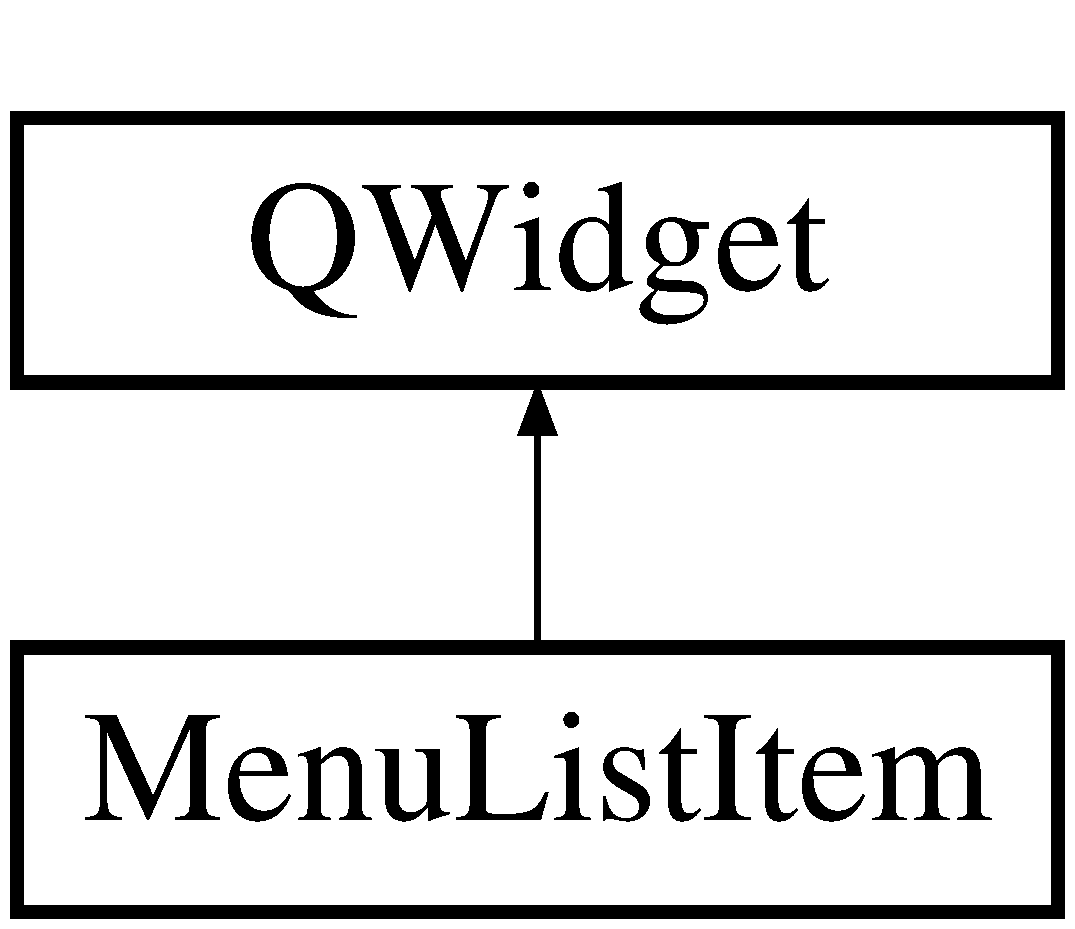
\includegraphics[height=2.000000cm]{classMenuListItem}
\end{center}
\end{figure}
\subsection*{Public Slots}
\begin{DoxyCompactItemize}
\item 
\hypertarget{classMenuListItem_a6bd73a8647102fc90684f4d056401a36}{void {\bfseries show\-Qty} (bool)}\label{classMenuListItem_a6bd73a8647102fc90684f4d056401a36}

\item 
\hypertarget{classMenuListItem_aa648340844394f75e14c02b29e99d290}{void {\bfseries reset\-Qty} ()}\label{classMenuListItem_aa648340844394f75e14c02b29e99d290}

\end{DoxyCompactItemize}
\subsection*{Signals}
\begin{DoxyCompactItemize}
\item 
\hypertarget{classMenuListItem_ac15f39d6de157c409990370b925d5e09}{void {\bfseries quantity\-Changed} (I\-Ds, Qty) const }\label{classMenuListItem_ac15f39d6de157c409990370b925d5e09}

\end{DoxyCompactItemize}
\subsection*{Public Member Functions}
\begin{DoxyCompactItemize}
\item 
\hypertarget{classMenuListItem_ac1bc2b6ef02b702d540b6afab14a00b1}{{\bfseries Menu\-List\-Item} (Q\-Widget $\ast$parent, Restaurant\-I\-D, \hyperlink{classMenuItem}{Menu\-Item})}\label{classMenuListItem_ac1bc2b6ef02b702d540b6afab14a00b1}

\item 
\hypertarget{classMenuListItem_a496e21bd4dcc0587a336f5a7afc7d4e1}{Qty {\bfseries get\-Qty} () const }\label{classMenuListItem_a496e21bd4dcc0587a336f5a7afc7d4e1}

\item 
\hypertarget{classMenuListItem_a90a0f8ba010149505c27e2573612e1b3}{I\-Ds {\bfseries get\-I\-Ds} () const }\label{classMenuListItem_a90a0f8ba010149505c27e2573612e1b3}

\item 
\hypertarget{classMenuListItem_a57215af3b031d16d4a7d336c87119bae}{void {\bfseries set\-Qty} (int)}\label{classMenuListItem_a57215af3b031d16d4a7d336c87119bae}

\end{DoxyCompactItemize}
\subsection*{Static Public Member Functions}
\begin{DoxyCompactItemize}
\item 
\hypertarget{classMenuListItem_a80a341261916a5c476ff773ad260e326}{static Q\-Size {\bfseries get\-Item\-Size\-Hint} ()}\label{classMenuListItem_a80a341261916a5c476ff773ad260e326}

\end{DoxyCompactItemize}


The documentation for this class was generated from the following files\-:\begin{DoxyCompactItemize}
\item 
/home/edt/\-C\-S1\-D/\-C\-S1\-D\-\_\-\-Fast\-\_\-\-Food\-\_\-\-Project/\-Fast\-Food\-Finder/src/widgets/menulistitem.\-hpp\item 
/home/edt/\-C\-S1\-D/\-C\-S1\-D\-\_\-\-Fast\-\_\-\-Food\-\_\-\-Project/\-Fast\-Food\-Finder/src/widgets/menulistitem.\-cpp\end{DoxyCompactItemize}

\hypertarget{classnsMyDblLinkList_1_1MyDblLinkList}{\section{ns\-My\-Dbl\-Link\-List\-:\-:My\-Dbl\-Link\-List$<$ Elem $>$ Class Template Reference}
\label{classnsMyDblLinkList_1_1MyDblLinkList}\index{ns\-My\-Dbl\-Link\-List\-::\-My\-Dbl\-Link\-List$<$ Elem $>$@{ns\-My\-Dbl\-Link\-List\-::\-My\-Dbl\-Link\-List$<$ Elem $>$}}
}
\subsection*{Classes}
\begin{DoxyCompactItemize}
\item 
class \hyperlink{classnsMyDblLinkList_1_1MyDblLinkList_1_1const__iterator}{const\-\_\-iterator}
\item 
class \hyperlink{classnsMyDblLinkList_1_1MyDblLinkList_1_1iterator}{iterator}
\end{DoxyCompactItemize}
\subsection*{Public Types}
\begin{DoxyCompactItemize}
\item 
enum {\bfseries Error\-Type} \{ {\bfseries I\-N\-V\-A\-L\-I\-D\-\_\-\-P\-O\-S\-I\-T\-I\-O\-N} = 100, 
{\bfseries L\-I\-S\-T\-\_\-\-E\-M\-P\-T\-Y} = 200, 
{\bfseries L\-I\-N\-K\-S\-\_\-\-I\-N\-V\-A\-L\-I\-D} = 300
 \}
\end{DoxyCompactItemize}
\subsection*{Public Member Functions}
\begin{DoxyCompactItemize}
\item 
\hyperlink{classnsMyDblLinkList_1_1MyDblLinkList_a3ea3bd9012c9a5512255f69f4e92a04e}{My\-Dbl\-Link\-List} (const \hyperlink{classnsMyDblLinkList_1_1MyDblLinkList}{My\-Dbl\-Link\-List} \&src)
\item 
\hyperlink{classnsMyDblLinkList_1_1MyDblLinkList}{My\-Dbl\-Link\-List} \& \hyperlink{classnsMyDblLinkList_1_1MyDblLinkList_adb891dd63c80ca95c0112c26dcc25ddf}{operator=} (const \hyperlink{classnsMyDblLinkList_1_1MyDblLinkList}{My\-Dbl\-Link\-List} \&src)
\item 
void \hyperlink{classnsMyDblLinkList_1_1MyDblLinkList_ad5adbd0d21f414c586fe2e4c29ecb968}{push\-\_\-back} (const Elem \&val)
\item 
Elem \& \hyperlink{classnsMyDblLinkList_1_1MyDblLinkList_a95d18c26b65859a681f8d3d21452c2b0}{front} (void) const 
\item 
void \hyperlink{classnsMyDblLinkList_1_1MyDblLinkList_a8fcb55e1577f9097b92d9edb34f70a3e}{pop\-\_\-front} (void)
\item 
Elem \& \hyperlink{classnsMyDblLinkList_1_1MyDblLinkList_a2258fc5ae8734bf096a4afff20c5e038}{back} (void) const 
\item 
void \hyperlink{classnsMyDblLinkList_1_1MyDblLinkList_a8f5da5782a5041ba160e9f3225cb05a7}{pop\-\_\-back} (void)
\item 
unsigned long \hyperlink{classnsMyDblLinkList_1_1MyDblLinkList_a04da8466e0d37191c782b234de856c3b}{size} (void) const 
\item 
bool \hyperlink{classnsMyDblLinkList_1_1MyDblLinkList_ab9c514b420e152d1f8d5f76f131f6b97}{is\-Empty} (void) const 
\item 
void \hyperlink{classnsMyDblLinkList_1_1MyDblLinkList_aed83c438f2b699771e5bf2ef9420beb1}{insert} (const Elem \&data, int position)
\item 
void \hyperlink{classnsMyDblLinkList_1_1MyDblLinkList_a864d0f3d60271a31a5ec1029f0e6ffdb}{erase} (int position)
\item 
void \hyperlink{classnsMyDblLinkList_1_1MyDblLinkList_a96e74ce8355d2e34714304ff6ed0e7a7}{add\-Sorted} (const Elem data)
\item 
Elem \& \hyperlink{classnsMyDblLinkList_1_1MyDblLinkList_ae9cc0f5a99478a0314e9a0d5ad48a296}{operator\mbox{[}$\,$\mbox{]}} (int position)
\item 
const Elem \& \hyperlink{classnsMyDblLinkList_1_1MyDblLinkList_a4ae1525359a5e499fda037f3a4ca3a08}{operator\mbox{[}$\,$\mbox{]}} (int position) const 
\item 
void \hyperlink{classnsMyDblLinkList_1_1MyDblLinkList_ae3e7df9c2643abe23a65a126d7e2174d}{print\-As\-Debug} (bool printeol=true, bool printcontent=false) const 
\item 
void \hyperlink{classnsMyDblLinkList_1_1MyDblLinkList_aaae80104b6b658008805cd3af410118a}{print} (bool printeol=true) const 
\item 
bool \hyperlink{classnsMyDblLinkList_1_1MyDblLinkList_a46ffecf0dc73999031da0b647cc17070}{validate} (void) const 
\item 
\hypertarget{classnsMyDblLinkList_1_1MyDblLinkList_a29a66301f515cc4deead1cc52be736ba}{\hyperlink{classnsMyDblLinkList_1_1MyDblLinkList_1_1iterator}{iterator} {\bfseries begin} ()}\label{classnsMyDblLinkList_1_1MyDblLinkList_a29a66301f515cc4deead1cc52be736ba}

\item 
\hypertarget{classnsMyDblLinkList_1_1MyDblLinkList_a16f416cf7e3e6b3efaabed7854ddd3af}{\hyperlink{classnsMyDblLinkList_1_1MyDblLinkList_1_1iterator}{iterator} {\bfseries end} ()}\label{classnsMyDblLinkList_1_1MyDblLinkList_a16f416cf7e3e6b3efaabed7854ddd3af}

\item 
\hypertarget{classnsMyDblLinkList_1_1MyDblLinkList_ab29e90f0b3aab8621ba2b5011314ee3a}{\hyperlink{classnsMyDblLinkList_1_1MyDblLinkList_1_1const__iterator}{const\-\_\-iterator} {\bfseries begin} () const }\label{classnsMyDblLinkList_1_1MyDblLinkList_ab29e90f0b3aab8621ba2b5011314ee3a}

\item 
\hypertarget{classnsMyDblLinkList_1_1MyDblLinkList_a72cbf109f49ed6cd0bd289b292bce75f}{\hyperlink{classnsMyDblLinkList_1_1MyDblLinkList_1_1const__iterator}{const\-\_\-iterator} {\bfseries end} () const }\label{classnsMyDblLinkList_1_1MyDblLinkList_a72cbf109f49ed6cd0bd289b292bce75f}

\end{DoxyCompactItemize}


\subsection{Constructor \& Destructor Documentation}
\hypertarget{classnsMyDblLinkList_1_1MyDblLinkList_a3ea3bd9012c9a5512255f69f4e92a04e}{\index{ns\-My\-Dbl\-Link\-List\-::\-My\-Dbl\-Link\-List@{ns\-My\-Dbl\-Link\-List\-::\-My\-Dbl\-Link\-List}!My\-Dbl\-Link\-List@{My\-Dbl\-Link\-List}}
\index{My\-Dbl\-Link\-List@{My\-Dbl\-Link\-List}!nsMyDblLinkList::MyDblLinkList@{ns\-My\-Dbl\-Link\-List\-::\-My\-Dbl\-Link\-List}}
\subsubsection[{My\-Dbl\-Link\-List}]{\setlength{\rightskip}{0pt plus 5cm}template$<$typename Elem $>$ {\bf ns\-My\-Dbl\-Link\-List\-::\-My\-Dbl\-Link\-List}$<$ Elem $>$\-::{\bf My\-Dbl\-Link\-List} (
\begin{DoxyParamCaption}
\item[{const {\bf My\-Dbl\-Link\-List}$<$ Elem $>$ \&}]{src}
\end{DoxyParamCaption}
)}}\label{classnsMyDblLinkList_1_1MyDblLinkList_a3ea3bd9012c9a5512255f69f4e92a04e}
Copy Contructor

\begin{DoxyAuthor}{Author}
edt (4/5/18)
\end{DoxyAuthor}

\begin{DoxyParams}{Parameters}
{\em src} & -\/ list being copied from \\
\hline
\end{DoxyParams}


\subsection{Member Function Documentation}
\hypertarget{classnsMyDblLinkList_1_1MyDblLinkList_a96e74ce8355d2e34714304ff6ed0e7a7}{\index{ns\-My\-Dbl\-Link\-List\-::\-My\-Dbl\-Link\-List@{ns\-My\-Dbl\-Link\-List\-::\-My\-Dbl\-Link\-List}!add\-Sorted@{add\-Sorted}}
\index{add\-Sorted@{add\-Sorted}!nsMyDblLinkList::MyDblLinkList@{ns\-My\-Dbl\-Link\-List\-::\-My\-Dbl\-Link\-List}}
\subsubsection[{add\-Sorted}]{\setlength{\rightskip}{0pt plus 5cm}template$<$typename Elem$>$ void {\bf ns\-My\-Dbl\-Link\-List\-::\-My\-Dbl\-Link\-List}$<$ Elem $>$\-::add\-Sorted (
\begin{DoxyParamCaption}
\item[{const Elem}]{data}
\end{DoxyParamCaption}
)}}\label{classnsMyDblLinkList_1_1MyDblLinkList_a96e74ce8355d2e34714304ff6ed0e7a7}
add\-Sorted -\/ adds element to a sorted list

\begin{DoxyAuthor}{Author}
edt (4/26/18)
\end{DoxyAuthor}

\begin{DoxyParams}{Parameters}
{\em data} & \\
\hline
\end{DoxyParams}
\hypertarget{classnsMyDblLinkList_1_1MyDblLinkList_a2258fc5ae8734bf096a4afff20c5e038}{\index{ns\-My\-Dbl\-Link\-List\-::\-My\-Dbl\-Link\-List@{ns\-My\-Dbl\-Link\-List\-::\-My\-Dbl\-Link\-List}!back@{back}}
\index{back@{back}!nsMyDblLinkList::MyDblLinkList@{ns\-My\-Dbl\-Link\-List\-::\-My\-Dbl\-Link\-List}}
\subsubsection[{back}]{\setlength{\rightskip}{0pt plus 5cm}template$<$typename Elem $>$ Elem \& {\bf ns\-My\-Dbl\-Link\-List\-::\-My\-Dbl\-Link\-List}$<$ Elem $>$\-::back (
\begin{DoxyParamCaption}
\item[{void}]{}
\end{DoxyParamCaption}
) const}}\label{classnsMyDblLinkList_1_1MyDblLinkList_a2258fc5ae8734bf096a4afff20c5e038}
back -\/ returns content of last element in queue, if any

\begin{DoxyAuthor}{Author}
edt (4/5/18)
\end{DoxyAuthor}
\begin{DoxyReturn}{Returns}
refernce to last list elememnt or throws exception if empty 
\end{DoxyReturn}
\hypertarget{classnsMyDblLinkList_1_1MyDblLinkList_a864d0f3d60271a31a5ec1029f0e6ffdb}{\index{ns\-My\-Dbl\-Link\-List\-::\-My\-Dbl\-Link\-List@{ns\-My\-Dbl\-Link\-List\-::\-My\-Dbl\-Link\-List}!erase@{erase}}
\index{erase@{erase}!nsMyDblLinkList::MyDblLinkList@{ns\-My\-Dbl\-Link\-List\-::\-My\-Dbl\-Link\-List}}
\subsubsection[{erase}]{\setlength{\rightskip}{0pt plus 5cm}template$<$typename Elem $>$ void {\bf ns\-My\-Dbl\-Link\-List\-::\-My\-Dbl\-Link\-List}$<$ Elem $>$\-::erase (
\begin{DoxyParamCaption}
\item[{int}]{position}
\end{DoxyParamCaption}
)}}\label{classnsMyDblLinkList_1_1MyDblLinkList_a864d0f3d60271a31a5ec1029f0e6ffdb}
erases list element at position specified

\begin{DoxyAuthor}{Author}
edt (4/25/18)
\end{DoxyAuthor}

\begin{DoxyParams}{Parameters}
{\em position} & -\/ element number to erase\\
\hline
\end{DoxyParams}
\begin{DoxyReturn}{Returns}
void 
\end{DoxyReturn}
\hypertarget{classnsMyDblLinkList_1_1MyDblLinkList_a95d18c26b65859a681f8d3d21452c2b0}{\index{ns\-My\-Dbl\-Link\-List\-::\-My\-Dbl\-Link\-List@{ns\-My\-Dbl\-Link\-List\-::\-My\-Dbl\-Link\-List}!front@{front}}
\index{front@{front}!nsMyDblLinkList::MyDblLinkList@{ns\-My\-Dbl\-Link\-List\-::\-My\-Dbl\-Link\-List}}
\subsubsection[{front}]{\setlength{\rightskip}{0pt plus 5cm}template$<$typename Elem $>$ Elem \& {\bf ns\-My\-Dbl\-Link\-List\-::\-My\-Dbl\-Link\-List}$<$ Elem $>$\-::front (
\begin{DoxyParamCaption}
\item[{void}]{}
\end{DoxyParamCaption}
) const}}\label{classnsMyDblLinkList_1_1MyDblLinkList_a95d18c26b65859a681f8d3d21452c2b0}
front -\/ returns content of first element in queue, if any

\begin{DoxyAuthor}{Author}
edt (4/5/18)
\end{DoxyAuthor}
\begin{DoxyReturn}{Returns}
refernce to first list elememnt or throws exception if empty 
\end{DoxyReturn}
\hypertarget{classnsMyDblLinkList_1_1MyDblLinkList_aed83c438f2b699771e5bf2ef9420beb1}{\index{ns\-My\-Dbl\-Link\-List\-::\-My\-Dbl\-Link\-List@{ns\-My\-Dbl\-Link\-List\-::\-My\-Dbl\-Link\-List}!insert@{insert}}
\index{insert@{insert}!nsMyDblLinkList::MyDblLinkList@{ns\-My\-Dbl\-Link\-List\-::\-My\-Dbl\-Link\-List}}
\subsubsection[{insert}]{\setlength{\rightskip}{0pt plus 5cm}template$<$typename Elem$>$ void {\bf ns\-My\-Dbl\-Link\-List\-::\-My\-Dbl\-Link\-List}$<$ Elem $>$\-::insert (
\begin{DoxyParamCaption}
\item[{const Elem \&}]{data, }
\item[{int}]{position}
\end{DoxyParamCaption}
)}}\label{classnsMyDblLinkList_1_1MyDblLinkList_aed83c438f2b699771e5bf2ef9420beb1}
insert element in list before specified element

\begin{DoxyAuthor}{Author}
edt (4/25/18)
\end{DoxyAuthor}

\begin{DoxyParams}{Parameters}
{\em data} & \\
\hline
{\em position} & \\
\hline
\end{DoxyParams}
\begin{DoxyReturn}{Returns}
void 
\end{DoxyReturn}
\hypertarget{classnsMyDblLinkList_1_1MyDblLinkList_ab9c514b420e152d1f8d5f76f131f6b97}{\index{ns\-My\-Dbl\-Link\-List\-::\-My\-Dbl\-Link\-List@{ns\-My\-Dbl\-Link\-List\-::\-My\-Dbl\-Link\-List}!is\-Empty@{is\-Empty}}
\index{is\-Empty@{is\-Empty}!nsMyDblLinkList::MyDblLinkList@{ns\-My\-Dbl\-Link\-List\-::\-My\-Dbl\-Link\-List}}
\subsubsection[{is\-Empty}]{\setlength{\rightskip}{0pt plus 5cm}template$<$typename Elem $>$ bool {\bf ns\-My\-Dbl\-Link\-List\-::\-My\-Dbl\-Link\-List}$<$ Elem $>$\-::is\-Empty (
\begin{DoxyParamCaption}
\item[{void}]{}
\end{DoxyParamCaption}
) const}}\label{classnsMyDblLinkList_1_1MyDblLinkList_ab9c514b420e152d1f8d5f76f131f6b97}
is\-Empty -\/ return true if queue empty

\begin{DoxyAuthor}{Author}
edt (4/5/18)
\end{DoxyAuthor}

\begin{DoxyParams}{Parameters}
{\em void} & \\
\hline
\end{DoxyParams}
\begin{DoxyReturn}{Returns}
bool -\/ true if queue empty, else false 
\end{DoxyReturn}
\hypertarget{classnsMyDblLinkList_1_1MyDblLinkList_adb891dd63c80ca95c0112c26dcc25ddf}{\index{ns\-My\-Dbl\-Link\-List\-::\-My\-Dbl\-Link\-List@{ns\-My\-Dbl\-Link\-List\-::\-My\-Dbl\-Link\-List}!operator=@{operator=}}
\index{operator=@{operator=}!nsMyDblLinkList::MyDblLinkList@{ns\-My\-Dbl\-Link\-List\-::\-My\-Dbl\-Link\-List}}
\subsubsection[{operator=}]{\setlength{\rightskip}{0pt plus 5cm}template$<$typename Elem $>$ {\bf My\-Dbl\-Link\-List}$<$ Elem $>$ \& {\bf ns\-My\-Dbl\-Link\-List\-::\-My\-Dbl\-Link\-List}$<$ Elem $>$\-::operator= (
\begin{DoxyParamCaption}
\item[{const {\bf My\-Dbl\-Link\-List}$<$ Elem $>$ \&}]{src}
\end{DoxyParamCaption}
)}}\label{classnsMyDblLinkList_1_1MyDblLinkList_adb891dd63c80ca95c0112c26dcc25ddf}
Copy Assignment Operator= -\/ copies the lesser of source queue elements or destination size of queue

\begin{DoxyAuthor}{Author}
edt (4/5/18)
\end{DoxyAuthor}

\begin{DoxyParams}{Parameters}
{\em rhs} & -\/ queue being assigned from\\
\hline
\end{DoxyParams}
\begin{DoxyReturn}{Returns}
\hyperlink{classnsMyDblLinkList_1_1MyDblLinkList}{My\-Dbl\-Link\-List}\& 
\end{DoxyReturn}
\hypertarget{classnsMyDblLinkList_1_1MyDblLinkList_ae9cc0f5a99478a0314e9a0d5ad48a296}{\index{ns\-My\-Dbl\-Link\-List\-::\-My\-Dbl\-Link\-List@{ns\-My\-Dbl\-Link\-List\-::\-My\-Dbl\-Link\-List}!operator\mbox{[}$\,$\mbox{]}@{operator[]}}
\index{operator\mbox{[}$\,$\mbox{]}@{operator[]}!nsMyDblLinkList::MyDblLinkList@{ns\-My\-Dbl\-Link\-List\-::\-My\-Dbl\-Link\-List}}
\subsubsection[{operator[]}]{\setlength{\rightskip}{0pt plus 5cm}template$<$typename Elem $>$ Elem \& {\bf ns\-My\-Dbl\-Link\-List\-::\-My\-Dbl\-Link\-List}$<$ Elem $>$\-::operator\mbox{[}$\,$\mbox{]} (
\begin{DoxyParamCaption}
\item[{int}]{position}
\end{DoxyParamCaption}
)}}\label{classnsMyDblLinkList_1_1MyDblLinkList_ae9cc0f5a99478a0314e9a0d5ad48a296}
overload subscript operator -\/ returns data at position soecified

\begin{DoxyAuthor}{Author}
edt (4/26/18)
\end{DoxyAuthor}

\begin{DoxyParams}{Parameters}
{\em position} & -\/ node number to return content\\
\hline
\end{DoxyParams}
\begin{DoxyReturn}{Returns}
reference to data at specified postion 
\end{DoxyReturn}
\hypertarget{classnsMyDblLinkList_1_1MyDblLinkList_a4ae1525359a5e499fda037f3a4ca3a08}{\index{ns\-My\-Dbl\-Link\-List\-::\-My\-Dbl\-Link\-List@{ns\-My\-Dbl\-Link\-List\-::\-My\-Dbl\-Link\-List}!operator\mbox{[}$\,$\mbox{]}@{operator[]}}
\index{operator\mbox{[}$\,$\mbox{]}@{operator[]}!nsMyDblLinkList::MyDblLinkList@{ns\-My\-Dbl\-Link\-List\-::\-My\-Dbl\-Link\-List}}
\subsubsection[{operator[]}]{\setlength{\rightskip}{0pt plus 5cm}template$<$typename Elem $>$ const Elem \& {\bf ns\-My\-Dbl\-Link\-List\-::\-My\-Dbl\-Link\-List}$<$ Elem $>$\-::operator\mbox{[}$\,$\mbox{]} (
\begin{DoxyParamCaption}
\item[{int}]{position}
\end{DoxyParamCaption}
) const}}\label{classnsMyDblLinkList_1_1MyDblLinkList_a4ae1525359a5e499fda037f3a4ca3a08}
overload subscript operator -\/ returns data at position soecified

\begin{DoxyAuthor}{Author}
edt (4/26/18)
\end{DoxyAuthor}

\begin{DoxyParams}{Parameters}
{\em position} & -\/ node number to return content\\
\hline
\end{DoxyParams}
\begin{DoxyReturn}{Returns}
const reference to data at specified postion 
\end{DoxyReturn}
\hypertarget{classnsMyDblLinkList_1_1MyDblLinkList_a8f5da5782a5041ba160e9f3225cb05a7}{\index{ns\-My\-Dbl\-Link\-List\-::\-My\-Dbl\-Link\-List@{ns\-My\-Dbl\-Link\-List\-::\-My\-Dbl\-Link\-List}!pop\-\_\-back@{pop\-\_\-back}}
\index{pop\-\_\-back@{pop\-\_\-back}!nsMyDblLinkList::MyDblLinkList@{ns\-My\-Dbl\-Link\-List\-::\-My\-Dbl\-Link\-List}}
\subsubsection[{pop\-\_\-back}]{\setlength{\rightskip}{0pt plus 5cm}template$<$typename Elem $>$ void {\bf ns\-My\-Dbl\-Link\-List\-::\-My\-Dbl\-Link\-List}$<$ Elem $>$\-::pop\-\_\-back (
\begin{DoxyParamCaption}
\item[{void}]{}
\end{DoxyParamCaption}
)}}\label{classnsMyDblLinkList_1_1MyDblLinkList_a8f5da5782a5041ba160e9f3225cb05a7}
pop\-\_\-back -\/ remove the lst element on the queue, if any

\begin{DoxyAuthor}{Author}
edt (4/5/18)
\end{DoxyAuthor}

\begin{DoxyParams}{Parameters}
{\em void} & \\
\hline
\end{DoxyParams}
\begin{DoxyReturn}{Returns}
void 
\end{DoxyReturn}
\hypertarget{classnsMyDblLinkList_1_1MyDblLinkList_a8fcb55e1577f9097b92d9edb34f70a3e}{\index{ns\-My\-Dbl\-Link\-List\-::\-My\-Dbl\-Link\-List@{ns\-My\-Dbl\-Link\-List\-::\-My\-Dbl\-Link\-List}!pop\-\_\-front@{pop\-\_\-front}}
\index{pop\-\_\-front@{pop\-\_\-front}!nsMyDblLinkList::MyDblLinkList@{ns\-My\-Dbl\-Link\-List\-::\-My\-Dbl\-Link\-List}}
\subsubsection[{pop\-\_\-front}]{\setlength{\rightskip}{0pt plus 5cm}template$<$typename Elem $>$ void {\bf ns\-My\-Dbl\-Link\-List\-::\-My\-Dbl\-Link\-List}$<$ Elem $>$\-::pop\-\_\-front (
\begin{DoxyParamCaption}
\item[{void}]{}
\end{DoxyParamCaption}
)}}\label{classnsMyDblLinkList_1_1MyDblLinkList_a8fcb55e1577f9097b92d9edb34f70a3e}
pop\-\_\-front -\/ remove the first element on the queue, if any

\begin{DoxyAuthor}{Author}
edt (4/5/18)
\end{DoxyAuthor}

\begin{DoxyParams}{Parameters}
{\em void} & \\
\hline
\end{DoxyParams}
\begin{DoxyReturn}{Returns}
void 
\end{DoxyReturn}
\hypertarget{classnsMyDblLinkList_1_1MyDblLinkList_aaae80104b6b658008805cd3af410118a}{\index{ns\-My\-Dbl\-Link\-List\-::\-My\-Dbl\-Link\-List@{ns\-My\-Dbl\-Link\-List\-::\-My\-Dbl\-Link\-List}!print@{print}}
\index{print@{print}!nsMyDblLinkList::MyDblLinkList@{ns\-My\-Dbl\-Link\-List\-::\-My\-Dbl\-Link\-List}}
\subsubsection[{print}]{\setlength{\rightskip}{0pt plus 5cm}template$<$typename Elem $>$ void {\bf ns\-My\-Dbl\-Link\-List\-::\-My\-Dbl\-Link\-List}$<$ Elem $>$\-::print (
\begin{DoxyParamCaption}
\item[{bool}]{printeol = {\ttfamily true}}
\end{DoxyParamCaption}
) const}}\label{classnsMyDblLinkList_1_1MyDblLinkList_aaae80104b6b658008805cd3af410118a}
print -\/ prints list and nodes

\begin{DoxyAuthor}{Author}
edt (4/5/18)
\end{DoxyAuthor}

\begin{DoxyParams}{Parameters}
{\em printeol} & -\/ true=output one line to console, false=print data on separate lines \\
\hline
\end{DoxyParams}
\hypertarget{classnsMyDblLinkList_1_1MyDblLinkList_ae3e7df9c2643abe23a65a126d7e2174d}{\index{ns\-My\-Dbl\-Link\-List\-::\-My\-Dbl\-Link\-List@{ns\-My\-Dbl\-Link\-List\-::\-My\-Dbl\-Link\-List}!print\-As\-Debug@{print\-As\-Debug}}
\index{print\-As\-Debug@{print\-As\-Debug}!nsMyDblLinkList::MyDblLinkList@{ns\-My\-Dbl\-Link\-List\-::\-My\-Dbl\-Link\-List}}
\subsubsection[{print\-As\-Debug}]{\setlength{\rightskip}{0pt plus 5cm}template$<$typename Elem $>$ void {\bf ns\-My\-Dbl\-Link\-List\-::\-My\-Dbl\-Link\-List}$<$ Elem $>$\-::print\-As\-Debug (
\begin{DoxyParamCaption}
\item[{bool}]{printeol = {\ttfamily true}, }
\item[{bool}]{printcontent = {\ttfamily false}}
\end{DoxyParamCaption}
) const}}\label{classnsMyDblLinkList_1_1MyDblLinkList_ae3e7df9c2643abe23a65a126d7e2174d}
print\-As\-Debug -\/ prints internal information about list and nodes

\begin{DoxyAuthor}{Author}
edt (4/5/18)
\end{DoxyAuthor}

\begin{DoxyParams}{Parameters}
{\em printeol} & -\/ true=output one line to console, false=print data on separate lines \\
\hline
{\em printcontent} & -\/ true= print elememnt data, if any \\
\hline
\end{DoxyParams}
\hypertarget{classnsMyDblLinkList_1_1MyDblLinkList_ad5adbd0d21f414c586fe2e4c29ecb968}{\index{ns\-My\-Dbl\-Link\-List\-::\-My\-Dbl\-Link\-List@{ns\-My\-Dbl\-Link\-List\-::\-My\-Dbl\-Link\-List}!push\-\_\-back@{push\-\_\-back}}
\index{push\-\_\-back@{push\-\_\-back}!nsMyDblLinkList::MyDblLinkList@{ns\-My\-Dbl\-Link\-List\-::\-My\-Dbl\-Link\-List}}
\subsubsection[{push\-\_\-back}]{\setlength{\rightskip}{0pt plus 5cm}template$<$typename Elem$>$ void {\bf ns\-My\-Dbl\-Link\-List\-::\-My\-Dbl\-Link\-List}$<$ Elem $>$\-::push\-\_\-back (
\begin{DoxyParamCaption}
\item[{const Elem \&}]{data}
\end{DoxyParamCaption}
)}}\label{classnsMyDblLinkList_1_1MyDblLinkList_ad5adbd0d21f414c586fe2e4c29ecb968}
add an element at end, if space available

\begin{DoxyAuthor}{Author}
edt (4/5/18)
\end{DoxyAuthor}

\begin{DoxyParams}{Parameters}
{\em data} & -\/ element content to add\\
\hline
\end{DoxyParams}
\begin{DoxyReturn}{Returns}
void 
\end{DoxyReturn}
\hypertarget{classnsMyDblLinkList_1_1MyDblLinkList_a04da8466e0d37191c782b234de856c3b}{\index{ns\-My\-Dbl\-Link\-List\-::\-My\-Dbl\-Link\-List@{ns\-My\-Dbl\-Link\-List\-::\-My\-Dbl\-Link\-List}!size@{size}}
\index{size@{size}!nsMyDblLinkList::MyDblLinkList@{ns\-My\-Dbl\-Link\-List\-::\-My\-Dbl\-Link\-List}}
\subsubsection[{size}]{\setlength{\rightskip}{0pt plus 5cm}template$<$typename Elem $>$ unsigned long {\bf ns\-My\-Dbl\-Link\-List\-::\-My\-Dbl\-Link\-List}$<$ Elem $>$\-::size (
\begin{DoxyParamCaption}
\item[{void}]{}
\end{DoxyParamCaption}
) const}}\label{classnsMyDblLinkList_1_1MyDblLinkList_a04da8466e0d37191c782b234de856c3b}
size -\/ return maximum number of elements in queue

\begin{DoxyAuthor}{Author}
edt (4/5/18)
\end{DoxyAuthor}

\begin{DoxyParams}{Parameters}
{\em void} & \\
\hline
\end{DoxyParams}
\begin{DoxyReturn}{Returns}
unsigned long 
\end{DoxyReturn}
\hypertarget{classnsMyDblLinkList_1_1MyDblLinkList_a46ffecf0dc73999031da0b647cc17070}{\index{ns\-My\-Dbl\-Link\-List\-::\-My\-Dbl\-Link\-List@{ns\-My\-Dbl\-Link\-List\-::\-My\-Dbl\-Link\-List}!validate@{validate}}
\index{validate@{validate}!nsMyDblLinkList::MyDblLinkList@{ns\-My\-Dbl\-Link\-List\-::\-My\-Dbl\-Link\-List}}
\subsubsection[{validate}]{\setlength{\rightskip}{0pt plus 5cm}template$<$typename Elem $>$ bool {\bf ns\-My\-Dbl\-Link\-List\-::\-My\-Dbl\-Link\-List}$<$ Elem $>$\-::validate (
\begin{DoxyParamCaption}
\item[{void}]{}
\end{DoxyParamCaption}
) const}}\label{classnsMyDblLinkList_1_1MyDblLinkList_a46ffecf0dc73999031da0b647cc17070}
validate -\/ checks forward and backward links, node count and first/last pointers

\begin{DoxyAuthor}{Author}
edt (4/26/18)
\end{DoxyAuthor}

\begin{DoxyParams}{Parameters}
{\em void} & \\
\hline
\end{DoxyParams}
\begin{DoxyReturn}{Returns}
bool -\/ trtue if all links consistant, false if an error exists 
\end{DoxyReturn}


The documentation for this class was generated from the following file\-:\begin{DoxyCompactItemize}
\item 
/home/edt/\-C\-S1\-D/\-C\-S1\-D\-\_\-\-Fast\-\_\-\-Food\-\_\-\-Project/\-Fast\-Food\-Finder/src/datastore/My\-Dbl\-Link\-List.\-hpp\end{DoxyCompactItemize}

\hypertarget{classNavBar}{\section{Nav\-Bar Class Reference}
\label{classNavBar}\index{Nav\-Bar@{Nav\-Bar}}
}
Inheritance diagram for Nav\-Bar\-:\begin{figure}[H]
\begin{center}
\leavevmode
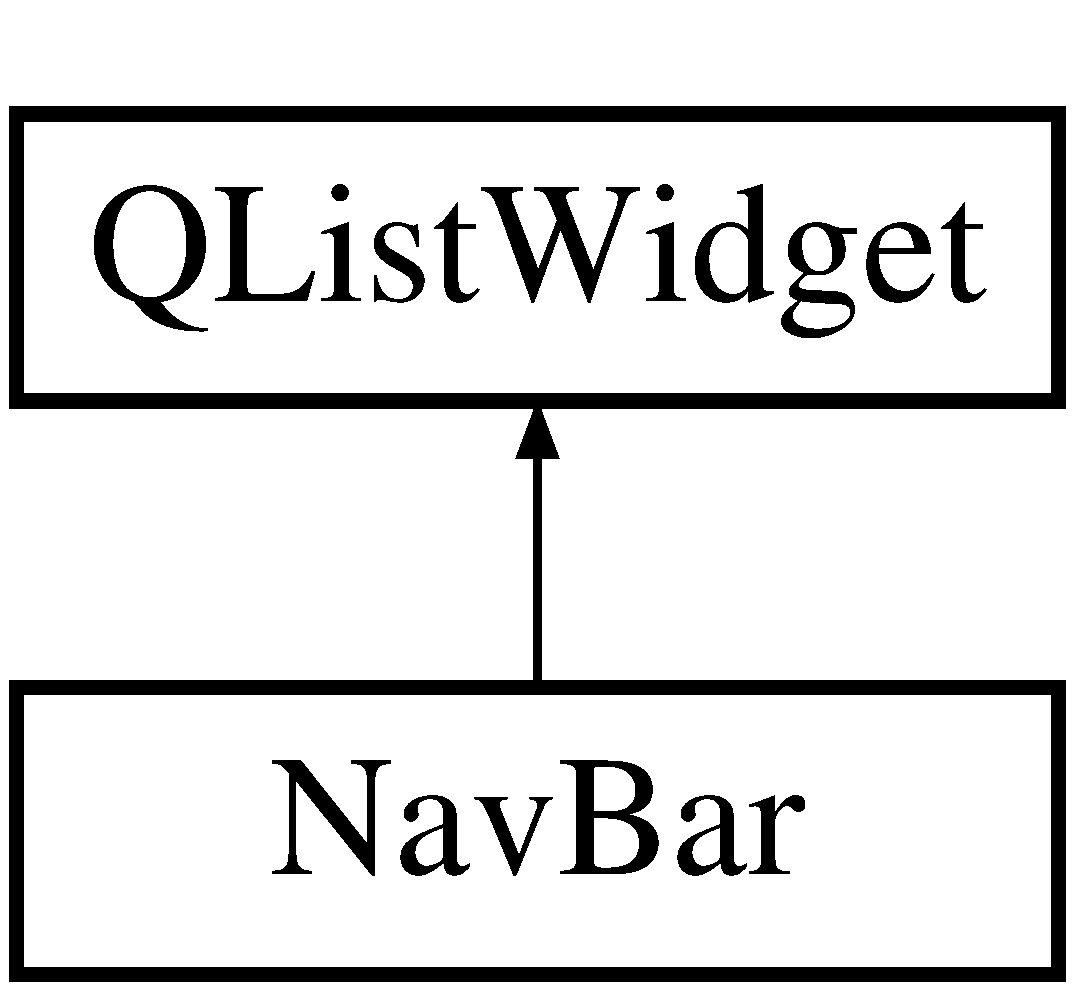
\includegraphics[height=2.000000cm]{classNavBar}
\end{center}
\end{figure}
\subsection*{Signals}
\begin{DoxyCompactItemize}
\item 
\hypertarget{classNavBar_a97d92d9d3a79f215b598fa507499707d}{void {\bfseries expand} ()}\label{classNavBar_a97d92d9d3a79f215b598fa507499707d}

\item 
\hypertarget{classNavBar_ab92546779d1fb94c21bbf2d7991faaa3}{void {\bfseries shrink} ()}\label{classNavBar_ab92546779d1fb94c21bbf2d7991faaa3}

\end{DoxyCompactItemize}
\subsection*{Public Member Functions}
\begin{DoxyCompactItemize}
\item 
\hyperlink{classNavBar_a988e7dc522635e792a5690613e80f042}{Nav\-Bar} (Q\-Widget $\ast$parent, int min\-Width, int max\-Width)
\begin{DoxyCompactList}\small\item\em Constructor. \end{DoxyCompactList}\item 
void \hyperlink{classNavBar_a02df27a57fc24bdf526e99b4fed6ad33}{set\-Height} (int)
\begin{DoxyCompactList}\small\item\em Set height of the bar. \end{DoxyCompactList}\item 
void \hyperlink{classNavBar_a8990d66058effa6cb08d1c86d9837443}{set\-Min\-Width} (int)
\begin{DoxyCompactList}\small\item\em Set minimum width of the bar. \end{DoxyCompactList}\item 
void \hyperlink{classNavBar_aa91680df575ef046c811cf665e763fa0}{set\-Max\-Width} (int)
\begin{DoxyCompactList}\small\item\em Set maximum width of the bar. \end{DoxyCompactList}\item 
void \hyperlink{classNavBar_afa07fd39fd9a51070186ed69ea563c89}{add\-Item} (Q\-String icon, Q\-String label)
\begin{DoxyCompactList}\small\item\em Add button to the bar. \end{DoxyCompactList}\end{DoxyCompactItemize}


\subsection{Detailed Description}
Provides an easy way to list clickable buttons. Currently, the class uses \char`\"{}\-Font Awesome 5 Free\char`\"{} for its icons.

To use\-: 
\begin{DoxyCode}
\hyperlink{classNavBar}{NavBar}* navbar = \textcolor{keyword}{new} \hyperlink{classNavBar_a988e7dc522635e792a5690613e80f042}{NavBar}(widget, 50, 100);
navbar->addItems(\textcolor{stringliteral}{"\(\backslash\)uffff"}, \textcolor{stringliteral}{"Button"});
\end{DoxyCode}


This will instantiate the bar under the widget with a minimum width of 50 and maximum width of 100. Then it will add a button with the icon \char`\"{}\textbackslash{}uffff\char`\"{} from the \char`\"{}\-Font Awesome 5 Free\char`\"{} font and a label \char`\"{}\-Button\char`\"{}.

\begin{DoxySeeAlso}{See Also}
\href{https://fontawesome.com/icons?d=gallery&m=free}{\tt Font Awesome icon reference} 
\end{DoxySeeAlso}


\subsection{Constructor \& Destructor Documentation}
\hypertarget{classNavBar_a988e7dc522635e792a5690613e80f042}{\index{Nav\-Bar@{Nav\-Bar}!Nav\-Bar@{Nav\-Bar}}
\index{Nav\-Bar@{Nav\-Bar}!NavBar@{Nav\-Bar}}
\subsubsection[{Nav\-Bar}]{\setlength{\rightskip}{0pt plus 5cm}Nav\-Bar\-::\-Nav\-Bar (
\begin{DoxyParamCaption}
\item[{Q\-Widget $\ast$}]{parent, }
\item[{int}]{min\-Width, }
\item[{int}]{max\-Width}
\end{DoxyParamCaption}
)}}\label{classNavBar_a988e7dc522635e792a5690613e80f042}


Constructor. 

Constructs a \hyperlink{classNavBar}{Nav\-Bar} object. It will resize its parent widget to whatever initial size it needs to be and its current height.


\begin{DoxyParams}{Parameters}
{\em parent} & The parent widget the bar will be contained in \\
\hline
{\em min\-Width} & Minimum width the bar will shrink to \\
\hline
{\em max\-Width} & Maximum width the bar will expand to \\
\hline
\end{DoxyParams}


\subsection{Member Function Documentation}
\hypertarget{classNavBar_afa07fd39fd9a51070186ed69ea563c89}{\index{Nav\-Bar@{Nav\-Bar}!add\-Item@{add\-Item}}
\index{add\-Item@{add\-Item}!NavBar@{Nav\-Bar}}
\subsubsection[{add\-Item}]{\setlength{\rightskip}{0pt plus 5cm}void Nav\-Bar\-::add\-Item (
\begin{DoxyParamCaption}
\item[{Q\-String}]{icon, }
\item[{Q\-String}]{label}
\end{DoxyParamCaption}
)}}\label{classNavBar_afa07fd39fd9a51070186ed69ea563c89}


Add button to the bar. 

Adds a new button to the bar using the given strings. Since \hyperlink{classNavBar}{Nav\-Bar} uses \char`\"{}\-Font Awesome 5 Free\char`\"{}, all unicode string icons should be represented by that font.


\begin{DoxyParams}{Parameters}
{\em icon} & The unicode representation (ex. ) of the icon using the\char`\"{}\-Font Awesome 5 Free\char`\"{} font \\
\hline
{\em label} & The label of the button \\
\hline
\end{DoxyParams}
\hypertarget{classNavBar_a02df27a57fc24bdf526e99b4fed6ad33}{\index{Nav\-Bar@{Nav\-Bar}!set\-Height@{set\-Height}}
\index{set\-Height@{set\-Height}!NavBar@{Nav\-Bar}}
\subsubsection[{set\-Height}]{\setlength{\rightskip}{0pt plus 5cm}void Nav\-Bar\-::set\-Height (
\begin{DoxyParamCaption}
\item[{int}]{height}
\end{DoxyParamCaption}
)}}\label{classNavBar_a02df27a57fc24bdf526e99b4fed6ad33}


Set height of the bar. 

Sets the height of the bar and its parent. Not changing its parent will end up cutting off the bar.


\begin{DoxyParams}{Parameters}
{\em height} & The new height of the bar and its parent \\
\hline
\end{DoxyParams}
\hypertarget{classNavBar_aa91680df575ef046c811cf665e763fa0}{\index{Nav\-Bar@{Nav\-Bar}!set\-Max\-Width@{set\-Max\-Width}}
\index{set\-Max\-Width@{set\-Max\-Width}!NavBar@{Nav\-Bar}}
\subsubsection[{set\-Max\-Width}]{\setlength{\rightskip}{0pt plus 5cm}void Nav\-Bar\-::set\-Max\-Width (
\begin{DoxyParamCaption}
\item[{int}]{width}
\end{DoxyParamCaption}
)}}\label{classNavBar_aa91680df575ef046c811cf665e763fa0}


Set maximum width of the bar. 

Sets the maximum width of the bar.


\begin{DoxyParams}{Parameters}
{\em width} & The new maximum width \\
\hline
\end{DoxyParams}
\hypertarget{classNavBar_a8990d66058effa6cb08d1c86d9837443}{\index{Nav\-Bar@{Nav\-Bar}!set\-Min\-Width@{set\-Min\-Width}}
\index{set\-Min\-Width@{set\-Min\-Width}!NavBar@{Nav\-Bar}}
\subsubsection[{set\-Min\-Width}]{\setlength{\rightskip}{0pt plus 5cm}void Nav\-Bar\-::set\-Min\-Width (
\begin{DoxyParamCaption}
\item[{int}]{width}
\end{DoxyParamCaption}
)}}\label{classNavBar_a8990d66058effa6cb08d1c86d9837443}


Set minimum width of the bar. 

Sets the minimum width of the bar.


\begin{DoxyParams}{Parameters}
{\em width} & The new minimum width \\
\hline
\end{DoxyParams}


The documentation for this class was generated from the following files\-:\begin{DoxyCompactItemize}
\item 
/home/edt/\-C\-S1\-D/\-C\-S1\-D\-\_\-\-Fast\-\_\-\-Food\-\_\-\-Project/\-Fast\-Food\-Finder/src/widgets/navbar.\-hpp\item 
/home/edt/\-C\-S1\-D/\-C\-S1\-D\-\_\-\-Fast\-\_\-\-Food\-\_\-\-Project/\-Fast\-Food\-Finder/src/widgets/navbar.\-cpp\end{DoxyCompactItemize}

\hypertarget{classNavItem}{\section{Nav\-Item Class Reference}
\label{classNavItem}\index{Nav\-Item@{Nav\-Item}}
}
Inheritance diagram for Nav\-Item\-:\begin{figure}[H]
\begin{center}
\leavevmode
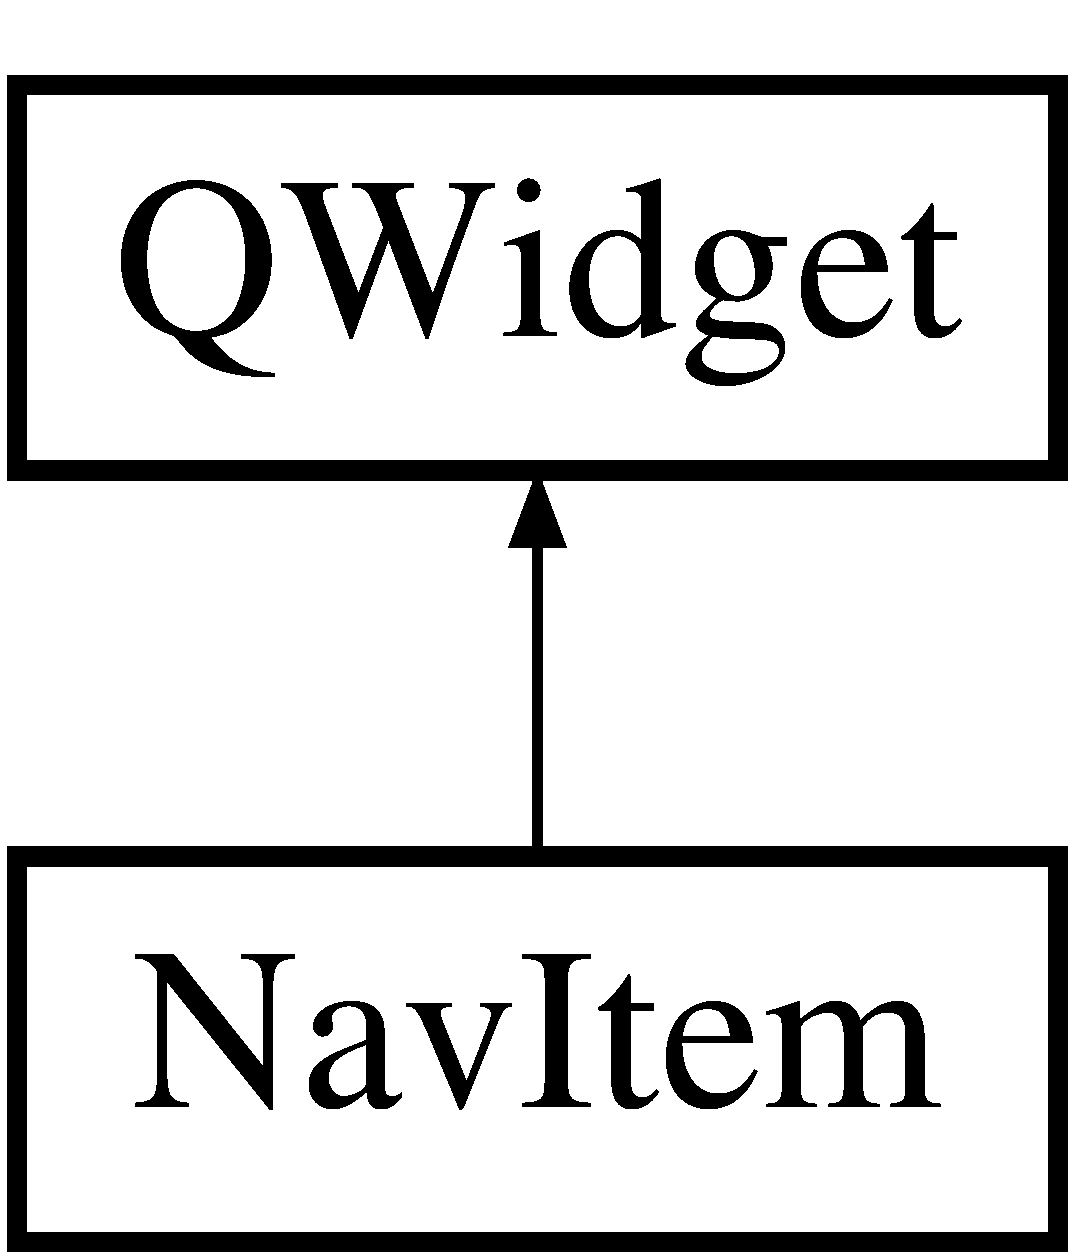
\includegraphics[height=2.000000cm]{classNavItem}
\end{center}
\end{figure}
\subsection*{Public Slots}
\begin{DoxyCompactItemize}
\item 
\hypertarget{classNavItem_af2b4677feec75195fa3dd0c44000d9cc}{void {\bfseries expand} () const }\label{classNavItem_af2b4677feec75195fa3dd0c44000d9cc}

\item 
\hypertarget{classNavItem_ada27101daf46eec0e5c56c5618b03c2a}{void {\bfseries shrink} () const }\label{classNavItem_ada27101daf46eec0e5c56c5618b03c2a}

\end{DoxyCompactItemize}
\subsection*{Public Member Functions}
\begin{DoxyCompactItemize}
\item 
\hypertarget{classNavItem_a2639e9b7df2859d0471d95192312d17b}{{\bfseries Nav\-Item} (Q\-List\-Widget $\ast$parent, Q\-String icon, Q\-String label)}\label{classNavItem_a2639e9b7df2859d0471d95192312d17b}

\end{DoxyCompactItemize}


The documentation for this class was generated from the following files\-:\begin{DoxyCompactItemize}
\item 
/home/edt/\-C\-S1\-D/\-C\-S1\-D\-\_\-\-Fast\-\_\-\-Food\-\_\-\-Project/\-Fast\-Food\-Finder/src/widgets/navitem.\-hpp\item 
/home/edt/\-C\-S1\-D/\-C\-S1\-D\-\_\-\-Fast\-\_\-\-Food\-\_\-\-Project/\-Fast\-Food\-Finder/src/widgets/navitem.\-cpp\end{DoxyCompactItemize}

\hypertarget{structnsMyDblLinkList_1_1Node}{\section{ns\-My\-Dbl\-Link\-List\-:\-:Node$<$ N\-T $>$ Struct Template Reference}
\label{structnsMyDblLinkList_1_1Node}\index{ns\-My\-Dbl\-Link\-List\-::\-Node$<$ N\-T $>$@{ns\-My\-Dbl\-Link\-List\-::\-Node$<$ N\-T $>$}}
}
\subsection*{Public Member Functions}
\begin{DoxyCompactItemize}
\item 
void \hyperlink{structnsMyDblLinkList_1_1Node_a1c685aa2d3b6235a0d158eeeb22e2e4f}{print\-As\-Debug} (bool printeol, bool printcontent) const 
\item 
void \hyperlink{structnsMyDblLinkList_1_1Node_ac0314baa23270d6bfb9c23826dcbd51a}{print} (bool printeol=true) const 
\item 
\hypertarget{structnsMyDblLinkList_1_1Node_a90e2de7612789da1dc60ac3a92d608e5}{{\bfseries Node} (const N\-T \&v=N\-T(), \hyperlink{structnsMyDblLinkList_1_1Node}{Node} $\ast$p=0, \hyperlink{structnsMyDblLinkList_1_1Node}{Node} $\ast$n=0)}\label{structnsMyDblLinkList_1_1Node_a90e2de7612789da1dc60ac3a92d608e5}

\end{DoxyCompactItemize}
\subsection*{Public Attributes}
\begin{DoxyCompactItemize}
\item 
\hypertarget{structnsMyDblLinkList_1_1Node_ae196dd88673937bbfec78aaba34b8633}{N\-T {\bfseries data}}\label{structnsMyDblLinkList_1_1Node_ae196dd88673937bbfec78aaba34b8633}

\item 
\hypertarget{structnsMyDblLinkList_1_1Node_a29c3ef4c274baee8254ba5b9590a12df}{\hyperlink{structnsMyDblLinkList_1_1Node}{Node} $\ast$ {\bfseries next}}\label{structnsMyDblLinkList_1_1Node_a29c3ef4c274baee8254ba5b9590a12df}

\item 
\hypertarget{structnsMyDblLinkList_1_1Node_a5186b20a38e08d11ff9507f933b92b63}{\hyperlink{structnsMyDblLinkList_1_1Node}{Node} $\ast$ {\bfseries prev}}\label{structnsMyDblLinkList_1_1Node_a5186b20a38e08d11ff9507f933b92b63}

\end{DoxyCompactItemize}


\subsection{Member Function Documentation}
\hypertarget{structnsMyDblLinkList_1_1Node_ac0314baa23270d6bfb9c23826dcbd51a}{\index{ns\-My\-Dbl\-Link\-List\-::\-Node@{ns\-My\-Dbl\-Link\-List\-::\-Node}!print@{print}}
\index{print@{print}!nsMyDblLinkList::Node@{ns\-My\-Dbl\-Link\-List\-::\-Node}}
\subsubsection[{print}]{\setlength{\rightskip}{0pt plus 5cm}template$<$typename N\-T $>$ void {\bf ns\-My\-Dbl\-Link\-List\-::\-Node}$<$ N\-T $>$\-::print (
\begin{DoxyParamCaption}
\item[{bool}]{printeol = {\ttfamily true}}
\end{DoxyParamCaption}
) const}}\label{structnsMyDblLinkList_1_1Node_ac0314baa23270d6bfb9c23826dcbd51a}
print -\/ prints node content

\begin{DoxyAuthor}{Author}
edt (4/5/18)
\end{DoxyAuthor}

\begin{DoxyParams}{Parameters}
{\em printeol} & -\/ true=output one line to console, false=print data on separate lines \\
\hline
{\em printcontent} & -\/ true= print elememnt data, if any \\
\hline
\end{DoxyParams}
\hypertarget{structnsMyDblLinkList_1_1Node_a1c685aa2d3b6235a0d158eeeb22e2e4f}{\index{ns\-My\-Dbl\-Link\-List\-::\-Node@{ns\-My\-Dbl\-Link\-List\-::\-Node}!print\-As\-Debug@{print\-As\-Debug}}
\index{print\-As\-Debug@{print\-As\-Debug}!nsMyDblLinkList::Node@{ns\-My\-Dbl\-Link\-List\-::\-Node}}
\subsubsection[{print\-As\-Debug}]{\setlength{\rightskip}{0pt plus 5cm}template$<$typename N\-T $>$ void {\bf ns\-My\-Dbl\-Link\-List\-::\-Node}$<$ N\-T $>$\-::print\-As\-Debug (
\begin{DoxyParamCaption}
\item[{bool}]{printeol, }
\item[{bool}]{printcontent}
\end{DoxyParamCaption}
) const}}\label{structnsMyDblLinkList_1_1Node_a1c685aa2d3b6235a0d158eeeb22e2e4f}
print\-As\-Debug -\/ prints internal information about node

\begin{DoxyAuthor}{Author}
edt (4/5/18)
\end{DoxyAuthor}

\begin{DoxyParams}{Parameters}
{\em printeol} & -\/ true=output one line to console, false=print data on separate lines \\
\hline
{\em printcontent} & -\/ true= print elememnt data, if any \\
\hline
\end{DoxyParams}


The documentation for this struct was generated from the following file\-:\begin{DoxyCompactItemize}
\item 
/home/edt/\-C\-S1\-D/\-C\-S1\-D\-\_\-\-Fast\-\_\-\-Food\-\_\-\-Project/\-Fast\-Food\-Finder/src/datastore/My\-Dbl\-Link\-List.\-hpp\end{DoxyCompactItemize}

\hypertarget{classRestaurant}{\section{Restaurant Class Reference}
\label{classRestaurant}\index{Restaurant@{Restaurant}}
}


{\ttfamily \#include $<$Restaurant.\-hpp$>$}

\subsection*{Public Member Functions}
\begin{DoxyCompactItemize}
\item 
\hypertarget{classRestaurant_a9ec8ac32f27c5e0b28376e5393bf1a46}{{\bfseries Restaurant} (const string \&Name, const float \&Distance)}\label{classRestaurant_a9ec8ac32f27c5e0b28376e5393bf1a46}

\item 
\hypertarget{classRestaurant_a509c9b7425703b48195ed2926a4e59e2}{{\bfseries Restaurant} (const \hyperlink{classRestaurant}{Restaurant} \&src)}\label{classRestaurant_a509c9b7425703b48195ed2926a4e59e2}

\item 
\hypertarget{classRestaurant_ac1f6dd1cc1e467a47134bd46330a0020}{\hyperlink{classRestaurant}{Restaurant} \& {\bfseries operator=} (const \hyperlink{classRestaurant}{Restaurant} \&rhs)}\label{classRestaurant_ac1f6dd1cc1e467a47134bd46330a0020}

\item 
\hypertarget{classRestaurant_a83808709ef46511be0ee73018b9e6d66}{const string \& {\bfseries Get\-Name} (void) const }\label{classRestaurant_a83808709ef46511be0ee73018b9e6d66}

\item 
\hypertarget{classRestaurant_a6035d861ae0ef8a8951002d6865b0362}{void {\bfseries Set\-Name} (const string \&New\-Name)}\label{classRestaurant_a6035d861ae0ef8a8951002d6865b0362}

\item 
\hypertarget{classRestaurant_aba8d743b610738dde66dd14d623b2dde}{int {\bfseries Get\-Number} (void) const }\label{classRestaurant_aba8d743b610738dde66dd14d623b2dde}

\item 
\hypertarget{classRestaurant_a918f12ce388683a75e6934b05f524a21}{const vector$<$ \hyperlink{classMenuItem}{Menu\-Item} $>$ \& {\bfseries Get\-Menu} (void) const }\label{classRestaurant_a918f12ce388683a75e6934b05f524a21}

\item 
\hypertarget{classRestaurant_aed44cf683bcec3c8d2c5f4f94f4ef936}{const vector\\*
$<$ \hyperlink{structRestaurantDistance}{Restaurant\-Distance} $>$ \& {\bfseries Get\-Distances} (void) const }\label{classRestaurant_aed44cf683bcec3c8d2c5f4f94f4ef936}

\item 
\hypertarget{classRestaurant_aedd3f76ea3d3cb361e9a44abe60e3a76}{float {\bfseries Get\-Purchase\-Amount} (void) const }\label{classRestaurant_aedd3f76ea3d3cb361e9a44abe60e3a76}

\item 
\hypertarget{classRestaurant_a3699a6975dfefc391189710525dbfa3d}{bool {\bfseries Mark\-Deleted} (bool Delete)}\label{classRestaurant_a3699a6975dfefc391189710525dbfa3d}

\item 
\hypertarget{classRestaurant_ad0a20e329cb53d0cf8d994f8dc105949}{bool {\bfseries Is\-Deleted} (void) const }\label{classRestaurant_ad0a20e329cb53d0cf8d994f8dc105949}

\item 
\hypertarget{classRestaurant_aca4ebabbbda736dac400d1ac5c6f0146}{bool {\bfseries Add\-Trip} (int Trip\-Number)}\label{classRestaurant_aca4ebabbbda736dac400d1ac5c6f0146}

\item 
\hypertarget{classRestaurant_a2f0687bea3f4d3ca11a8fdc704fdfa36}{int {\bfseries Add\-Cust\-Count} (void)}\label{classRestaurant_a2f0687bea3f4d3ca11a8fdc704fdfa36}

\item 
\hypertarget{classRestaurant_aa56bf703c6d0c8e03117befeeda61377}{float {\bfseries Add\-Purchase\-Price} (float Purchase\-Amount)}\label{classRestaurant_aa56bf703c6d0c8e03117befeeda61377}

\item 
\hypertarget{classRestaurant_ae67e3528af9514e3bdf01f10db874586}{float {\bfseries Get\-Dist\-Saddleback} (void) const }\label{classRestaurant_ae67e3528af9514e3bdf01f10db874586}

\item 
\hypertarget{classRestaurant_ae709b1c3f23b25dd27c9f526dc536fa8}{void {\bfseries Add\-Menu\-Item} (const string \&Name, const float \&Price)}\label{classRestaurant_ae709b1c3f23b25dd27c9f526dc536fa8}

\item 
\hypertarget{classRestaurant_af483bb828a00f12643e366ecd9766565}{\hyperlink{classMenuItem}{Menu\-Item} \& {\bfseries Find\-Menu\-Itemby\-Number} (int Number)}\label{classRestaurant_af483bb828a00f12643e366ecd9766565}

\item 
bool \hyperlink{classRestaurant_aa303b241946e96f7a4316a30ac6d31df}{Print\-As\-Debug} (bool print\-\_\-endl) const 
\end{DoxyCompactItemize}
\subsection*{Friends}
\begin{DoxyCompactItemize}
\item 
\hypertarget{classRestaurant_af6d4a4f1eb97251a24add34c6978faa2}{class {\bfseries Restaurant\-Data\-Store}}\label{classRestaurant_af6d4a4f1eb97251a24add34c6978faa2}

\item 
ostream \& \hyperlink{classRestaurant_affbf9125e0ad7687db2345ea02c61607}{operator$<$$<$} (ostream \&os, const \hyperlink{classRestaurant}{Restaurant} \&restaurant)
\end{DoxyCompactItemize}


\subsection{Detailed Description}
Internal datastore for \hyperlink{classRestaurant}{Restaurant} Objects

\begin{DoxyAuthor}{Author}
edt 
\end{DoxyAuthor}


\subsection{Member Function Documentation}
\hypertarget{classRestaurant_aa303b241946e96f7a4316a30ac6d31df}{\index{Restaurant@{Restaurant}!Print\-As\-Debug@{Print\-As\-Debug}}
\index{Print\-As\-Debug@{Print\-As\-Debug}!Restaurant@{Restaurant}}
\subsubsection[{Print\-As\-Debug}]{\setlength{\rightskip}{0pt plus 5cm}bool Restaurant\-::\-Print\-As\-Debug (
\begin{DoxyParamCaption}
\item[{bool}]{print\-\_\-endl}
\end{DoxyParamCaption}
) const}}\label{classRestaurant_aa303b241946e96f7a4316a30ac6d31df}
print the value of the object for external display

\begin{DoxyAuthor}{Author}
edt (2/7/18)
\end{DoxyAuthor}

\begin{DoxyParams}{Parameters}
{\em print\-\_\-endl} & \\
\hline
\end{DoxyParams}
\begin{DoxyReturn}{Returns}
bool 
\end{DoxyReturn}


\subsection{Friends And Related Function Documentation}
\hypertarget{classRestaurant_affbf9125e0ad7687db2345ea02c61607}{\index{Restaurant@{Restaurant}!operator$<$$<$@{operator$<$$<$}}
\index{operator$<$$<$@{operator$<$$<$}!Restaurant@{Restaurant}}
\subsubsection[{operator$<$$<$}]{\setlength{\rightskip}{0pt plus 5cm}ostream\& operator$<$$<$ (
\begin{DoxyParamCaption}
\item[{ostream \&}]{os, }
\item[{const {\bf Restaurant} \&}]{restaurant}
\end{DoxyParamCaption}
)\hspace{0.3cm}{\ttfamily [friend]}}}\label{classRestaurant_affbf9125e0ad7687db2345ea02c61607}
Overloaded operator $<$$<$ to print the contents of an \hyperlink{classUser}{User} object

\begin{DoxyAuthor}{Author}
edt (2/7/18)
\end{DoxyAuthor}

\begin{DoxyParams}{Parameters}
{\em os} & \\
\hline
{\em \hyperlink{classRestaurant}{Restaurant}} & \\
\hline
\end{DoxyParams}
\begin{DoxyReturn}{Returns}
ostream\& 
\end{DoxyReturn}


The documentation for this class was generated from the following files\-:\begin{DoxyCompactItemize}
\item 
/home/edt/\-C\-S1\-D/\-C\-S1\-D\-\_\-\-Fast\-\_\-\-Food\-\_\-\-Project/\-Fast\-Food\-Finder/src/datastore/Restaurant.\-hpp\item 
/home/edt/\-C\-S1\-D/\-C\-S1\-D\-\_\-\-Fast\-\_\-\-Food\-\_\-\-Project/\-Fast\-Food\-Finder/src/datastore/Restaurant.\-cpp\end{DoxyCompactItemize}

\hypertarget{classRestaurantDataStore}{\section{Restaurant\-Data\-Store Class Reference}
\label{classRestaurantDataStore}\index{Restaurant\-Data\-Store@{Restaurant\-Data\-Store}}
}


{\ttfamily \#include $<$Restaurant\-Data\-Store.\-hpp$>$}

\subsection*{Public Member Functions}
\begin{DoxyCompactItemize}
\item 
\hyperlink{classRestaurantDataStore_af8f86d29e3a76e964cc800ca6ad558fc}{Restaurant\-Data\-Store} ()
\item 
virtual \hyperlink{classRestaurantDataStore_ad40b37de8908fab03e7b224ae8f90f28}{$\sim$\-Restaurant\-Data\-Store} ()
\item 
void \hyperlink{classRestaurantDataStore_ad93c185aa70e70775844d4e21402ec4d}{print\-As\-Debug} (bool printeol, bool printcontent) const 
\item 
\hyperlink{classRestaurant}{Restaurant} \& \hyperlink{classRestaurantDataStore_a23cc1d33c1f53a477a6fadc8e8894757}{Findby\-Number} (int Number)
\item 
void \hyperlink{classRestaurantDataStore_a110407e1b764b7eba249093358730aee}{load} (const string path, bool Items\-Are\-Additional=false)
\item 
void \hyperlink{classRestaurantDataStore_af0a228a38c8a77ff4d03413e36e7813b}{save} (const string path)
\item 
void \hyperlink{classRestaurantDataStore_abdd5fbf8695de1f8ec4de4238d0705a3}{load\-\_\-additional} (const string path)
\end{DoxyCompactItemize}
\subsection*{Public Attributes}
\begin{DoxyCompactItemize}
\item 
\hypertarget{classRestaurantDataStore_a37965da233518c654c93108824fb64b8}{std\-::list$<$ \hyperlink{classRestaurant}{Restaurant} $>$ {\bfseries list}}\label{classRestaurantDataStore_a37965da233518c654c93108824fb64b8}

\end{DoxyCompactItemize}


\subsection{Detailed Description}
\hyperlink{classRestaurantDataStore}{Restaurant\-Data\-Store} -\/ internal storage for \hyperlink{classRestaurant}{Restaurant} objects

\begin{DoxyAuthor}{Author}
edt (3/25/19) 
\end{DoxyAuthor}


\subsection{Constructor \& Destructor Documentation}
\hypertarget{classRestaurantDataStore_af8f86d29e3a76e964cc800ca6ad558fc}{\index{Restaurant\-Data\-Store@{Restaurant\-Data\-Store}!Restaurant\-Data\-Store@{Restaurant\-Data\-Store}}
\index{Restaurant\-Data\-Store@{Restaurant\-Data\-Store}!RestaurantDataStore@{Restaurant\-Data\-Store}}
\subsubsection[{Restaurant\-Data\-Store}]{\setlength{\rightskip}{0pt plus 5cm}Restaurant\-Data\-Store\-::\-Restaurant\-Data\-Store (
\begin{DoxyParamCaption}
{}
\end{DoxyParamCaption}
)}}\label{classRestaurantDataStore_af8f86d29e3a76e964cc800ca6ad558fc}
default constuctor

\begin{DoxyAuthor}{Author}
edt (3/25/19) 
\end{DoxyAuthor}
\hypertarget{classRestaurantDataStore_ad40b37de8908fab03e7b224ae8f90f28}{\index{Restaurant\-Data\-Store@{Restaurant\-Data\-Store}!$\sim$\-Restaurant\-Data\-Store@{$\sim$\-Restaurant\-Data\-Store}}
\index{$\sim$\-Restaurant\-Data\-Store@{$\sim$\-Restaurant\-Data\-Store}!RestaurantDataStore@{Restaurant\-Data\-Store}}
\subsubsection[{$\sim$\-Restaurant\-Data\-Store}]{\setlength{\rightskip}{0pt plus 5cm}Restaurant\-Data\-Store\-::$\sim$\-Restaurant\-Data\-Store (
\begin{DoxyParamCaption}
{}
\end{DoxyParamCaption}
)\hspace{0.3cm}{\ttfamily [virtual]}}}\label{classRestaurantDataStore_ad40b37de8908fab03e7b224ae8f90f28}
\hyperlink{classRestaurantDataStore_ad40b37de8908fab03e7b224ae8f90f28}{Restaurant\-Data\-Store\-::$\sim$\-Restaurant\-Data\-Store} -\/ Destructor

\begin{DoxyAuthor}{Author}
edt (3/25/19) 
\end{DoxyAuthor}


\subsection{Member Function Documentation}
\hypertarget{classRestaurantDataStore_a23cc1d33c1f53a477a6fadc8e8894757}{\index{Restaurant\-Data\-Store@{Restaurant\-Data\-Store}!Findby\-Number@{Findby\-Number}}
\index{Findby\-Number@{Findby\-Number}!RestaurantDataStore@{Restaurant\-Data\-Store}}
\subsubsection[{Findby\-Number}]{\setlength{\rightskip}{0pt plus 5cm}{\bf Restaurant} \& Restaurant\-Data\-Store\-::\-Findby\-Number (
\begin{DoxyParamCaption}
\item[{int}]{Number}
\end{DoxyParamCaption}
)}}\label{classRestaurantDataStore_a23cc1d33c1f53a477a6fadc8e8894757}
\hyperlink{classRestaurantDataStore_a23cc1d33c1f53a477a6fadc8e8894757}{Restaurant\-Data\-Store\-::\-Findby\-Number} -\/ locate \hyperlink{classRestaurant}{Restaurant} in datastore by number

\begin{DoxyAuthor}{Author}
edt (3/25/19)
\end{DoxyAuthor}

\begin{DoxyParams}{Parameters}
{\em Number} & -\/ number to locate\\
\hline
\end{DoxyParams}
\begin{DoxyReturn}{Returns}
\hyperlink{classRestaurant}{Restaurant}\& -\/ pointer to \hyperlink{classRestaurant}{Restaurant} or N\-U\-L\-L if not found 
\end{DoxyReturn}
\hypertarget{classRestaurantDataStore_a110407e1b764b7eba249093358730aee}{\index{Restaurant\-Data\-Store@{Restaurant\-Data\-Store}!load@{load}}
\index{load@{load}!RestaurantDataStore@{Restaurant\-Data\-Store}}
\subsubsection[{load}]{\setlength{\rightskip}{0pt plus 5cm}void Restaurant\-Data\-Store\-::load (
\begin{DoxyParamCaption}
\item[{const string}]{path, }
\item[{bool}]{Items\-Are\-Additional = {\ttfamily false}}
\end{DoxyParamCaption}
)}}\label{classRestaurantDataStore_a110407e1b764b7eba249093358730aee}
\hyperlink{classRestaurantDataStore_a110407e1b764b7eba249093358730aee}{Restaurant\-Data\-Store\-::load} -\/ get object data from file

\begin{DoxyAuthor}{Author}
edt (3/25/19)
\end{DoxyAuthor}

\begin{DoxyParams}{Parameters}
{\em path} & -\/ location of C\-S\-V file to load \\
\hline
{\em Items\-Are\-Additional} & -\/ add items to existing datastore \\
\hline
\end{DoxyParams}
\hypertarget{classRestaurantDataStore_abdd5fbf8695de1f8ec4de4238d0705a3}{\index{Restaurant\-Data\-Store@{Restaurant\-Data\-Store}!load\-\_\-additional@{load\-\_\-additional}}
\index{load\-\_\-additional@{load\-\_\-additional}!RestaurantDataStore@{Restaurant\-Data\-Store}}
\subsubsection[{load\-\_\-additional}]{\setlength{\rightskip}{0pt plus 5cm}void Restaurant\-Data\-Store\-::load\-\_\-additional (
\begin{DoxyParamCaption}
\item[{const string}]{path}
\end{DoxyParamCaption}
)}}\label{classRestaurantDataStore_abdd5fbf8695de1f8ec4de4238d0705a3}
\hyperlink{classRestaurantDataStore_abdd5fbf8695de1f8ec4de4238d0705a3}{Restaurant\-Data\-Store\-::load\-\_\-additional} -\/ helper function to add Restaurants to existing datastore

\begin{DoxyAuthor}{Author}
edt (3/25/19)
\end{DoxyAuthor}

\begin{DoxyParams}{Parameters}
{\em path} & -\/ location of C\-S\-V file to load \\
\hline
\end{DoxyParams}
\hypertarget{classRestaurantDataStore_ad93c185aa70e70775844d4e21402ec4d}{\index{Restaurant\-Data\-Store@{Restaurant\-Data\-Store}!print\-As\-Debug@{print\-As\-Debug}}
\index{print\-As\-Debug@{print\-As\-Debug}!RestaurantDataStore@{Restaurant\-Data\-Store}}
\subsubsection[{print\-As\-Debug}]{\setlength{\rightskip}{0pt plus 5cm}void Restaurant\-Data\-Store\-::print\-As\-Debug (
\begin{DoxyParamCaption}
\item[{bool}]{printeol, }
\item[{bool}]{printcontent}
\end{DoxyParamCaption}
) const}}\label{classRestaurantDataStore_ad93c185aa70e70775844d4e21402ec4d}
\hyperlink{classRestaurantDataStore_ad93c185aa70e70775844d4e21402ec4d}{Restaurant\-Data\-Store\-::print\-As\-Debug} -\/ helper function to print internal state of all objects in datastore

\begin{DoxyAuthor}{Author}
edt (3/25/19)
\end{DoxyAuthor}

\begin{DoxyParams}{Parameters}
{\em printeol} & -\/ print end of lines after each data element \\
\hline
{\em printcontent} & -\/ print internal data of Restaurants \\
\hline
\end{DoxyParams}
\hypertarget{classRestaurantDataStore_af0a228a38c8a77ff4d03413e36e7813b}{\index{Restaurant\-Data\-Store@{Restaurant\-Data\-Store}!save@{save}}
\index{save@{save}!RestaurantDataStore@{Restaurant\-Data\-Store}}
\subsubsection[{save}]{\setlength{\rightskip}{0pt plus 5cm}void Restaurant\-Data\-Store\-::save (
\begin{DoxyParamCaption}
\item[{const string}]{path}
\end{DoxyParamCaption}
)}}\label{classRestaurantDataStore_af0a228a38c8a77ff4d03413e36e7813b}
\hyperlink{classRestaurantDataStore_af0a228a38c8a77ff4d03413e36e7813b}{Restaurant\-Data\-Store\-::save} -\/ save objects to external C\-S\-V file

\begin{DoxyAuthor}{Author}
edt (3/25/19)
\end{DoxyAuthor}

\begin{DoxyParams}{Parameters}
{\em path} & -\/ location of external file (will be overwritten) \\
\hline
\end{DoxyParams}


The documentation for this class was generated from the following files\-:\begin{DoxyCompactItemize}
\item 
/home/edt/\-C\-S1\-D/\-C\-S1\-D\-\_\-\-Fast\-\_\-\-Food\-\_\-\-Project/\-Fast\-Food\-Finder/src/datastore/Restaurant\-Data\-Store.\-hpp\item 
/home/edt/\-C\-S1\-D/\-C\-S1\-D\-\_\-\-Fast\-\_\-\-Food\-\_\-\-Project/\-Fast\-Food\-Finder/src/datastore/Restaurant\-Data\-Store.\-cpp\end{DoxyCompactItemize}

\hypertarget{structRestaurantDistance}{\section{Restaurant\-Distance Struct Reference}
\label{structRestaurantDistance}\index{Restaurant\-Distance@{Restaurant\-Distance}}
}


{\ttfamily \#include $<$Restaurant.\-hpp$>$}

\subsection*{Public Attributes}
\begin{DoxyCompactItemize}
\item 
\hypertarget{structRestaurantDistance_afb739d6fb9ec442a677862441661e72a}{int {\bfseries m\-\_\-n\-Restaurant\-Number}}\label{structRestaurantDistance_afb739d6fb9ec442a677862441661e72a}

\item 
\hypertarget{structRestaurantDistance_a075d62cf404beeb176b00e99477aecc2}{float {\bfseries m\-\_\-f\-Distance\-Miles}}\label{structRestaurantDistance_a075d62cf404beeb176b00e99477aecc2}

\end{DoxyCompactItemize}


\subsection{Detailed Description}
\hyperlink{structRestaurantDistance}{Restaurant\-Distance} -\/ container for restaurant numbers and their related distances from the containing \hyperlink{classRestaurant}{Restaurant}

\begin{DoxyAuthor}{Author}
edt (3/25/19) 
\end{DoxyAuthor}


The documentation for this struct was generated from the following file\-:\begin{DoxyCompactItemize}
\item 
/home/edt/\-C\-S1\-D/\-C\-S1\-D\-\_\-\-Fast\-\_\-\-Food\-\_\-\-Project/\-Fast\-Food\-Finder/src/datastore/Restaurant.\-hpp\end{DoxyCompactItemize}

\hypertarget{classRestaurantList}{\section{Restaurant\-List Class Reference}
\label{classRestaurantList}\index{Restaurant\-List@{Restaurant\-List}}
}
Inheritance diagram for Restaurant\-List\-:\begin{figure}[H]
\begin{center}
\leavevmode
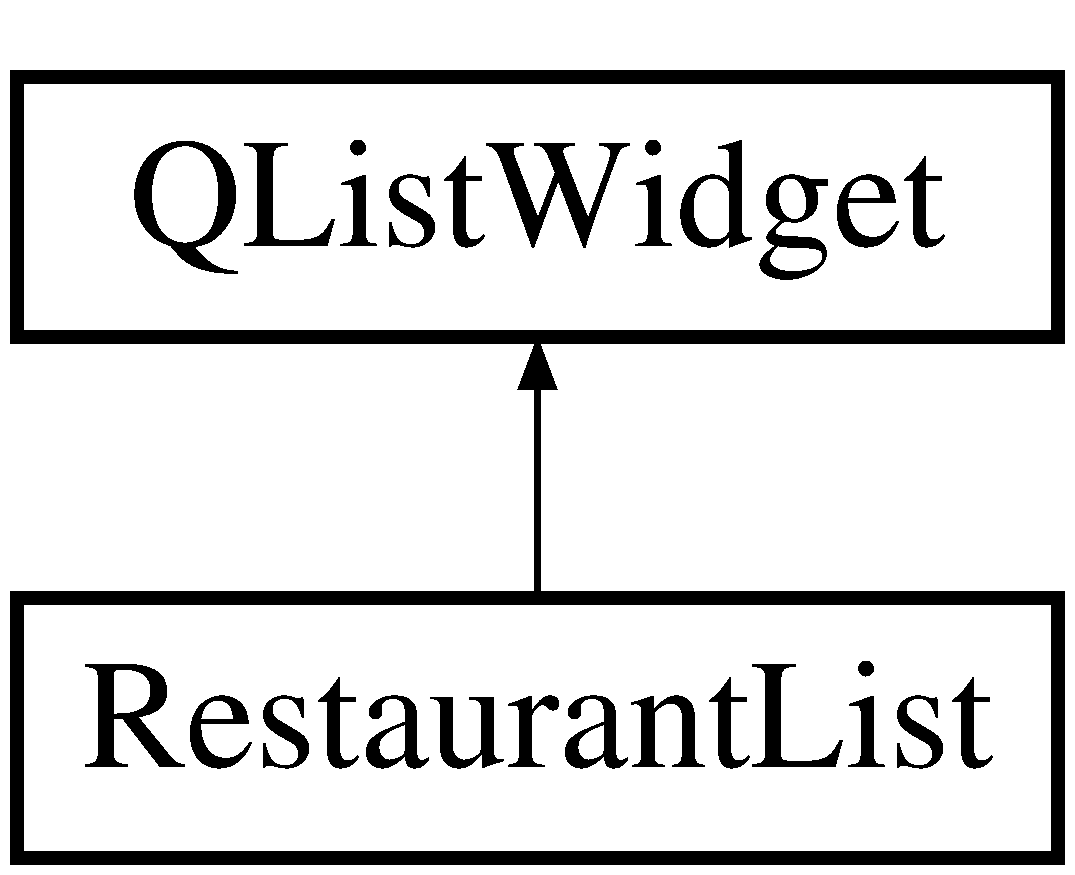
\includegraphics[height=2.000000cm]{classRestaurantList}
\end{center}
\end{figure}
\subsection*{Signals}
\begin{DoxyCompactItemize}
\item 
\hypertarget{classRestaurantList_a288c89af96c8ac2c537b51f8d8a565ed}{void {\bfseries current\-Restaurant\-Changed} (Restaurant\-I\-D) const }\label{classRestaurantList_a288c89af96c8ac2c537b51f8d8a565ed}

\end{DoxyCompactItemize}
\subsection*{Public Member Functions}
\begin{DoxyCompactItemize}
\item 
\hyperlink{classRestaurantList_a233e9bb9c25a1531d754459f8e0eef81}{Restaurant\-List} (Q\-Widget $\ast$parent)
\begin{DoxyCompactList}\small\item\em Constructor. \end{DoxyCompactList}\item 
Restaurant\-I\-D \hyperlink{classRestaurantList_a4427f0f8f4b09d830de4687588b2fd72}{get\-Selected} () const 
\begin{DoxyCompactList}\small\item\em Get selected restaurant I\-D. \end{DoxyCompactList}\item 
{\footnotesize template$<$typename Container $>$ }\\void \hyperlink{classRestaurantList_a72fce6ff45c3cceaa794d32e9118fe2d}{get\-Restaurant\-I\-Ds} (Container \&) const 
\begin{DoxyCompactList}\small\item\em Get all restaurant I\-Ds. \end{DoxyCompactList}\item 
void \hyperlink{classRestaurantList_a174ca2fb41584d6e674cfa1c79833fbd}{add\-Item} (const \hyperlink{classRestaurant}{Restaurant} \&)
\begin{DoxyCompactList}\small\item\em Add restaurant to list. \end{DoxyCompactList}\item 
{\footnotesize template$<$typename Iterator $>$ }\\void \hyperlink{classRestaurantList_aeb4247604bf1ea14b33878c7ffc43ac4}{add\-Items} (Iterator begin, Iterator end)
\begin{DoxyCompactList}\small\item\em Add multiple restaurants to the list. \end{DoxyCompactList}\item 
void \hyperlink{classRestaurantList_ae29016217ee9c4d9517f5b384feb450c}{remove\-Item} (const \hyperlink{classRestaurant}{Restaurant} \&)
\begin{DoxyCompactList}\small\item\em Remove restaurant from list. \end{DoxyCompactList}\item 
{\footnotesize template$<$typename Iterator $>$ }\\void \hyperlink{classRestaurantList_a32c2c4d381a0c1f37a6090d6a7c4f276}{remove\-Items} (Iterator begin, Iterator end)
\begin{DoxyCompactList}\small\item\em Remove multiple restaurants from the list. \end{DoxyCompactList}\item 
void \hyperlink{classRestaurantList_a5c9d824123dc0001ee091c6f86ede859}{show\-Hidden} (bool)
\begin{DoxyCompactList}\small\item\em Show hidden restaurants. \end{DoxyCompactList}\end{DoxyCompactItemize}


\subsection{Detailed Description}
Provides a simple way to list restaurant objects.

To use\-: 
\begin{DoxyCode}
\hyperlink{classRestaurantList}{RestaurantList}* list = \textcolor{keyword}{new} \hyperlink{classRestaurantList_a233e9bb9c25a1531d754459f8e0eef81}{RestaurantList}(widget);
list->\hyperlink{classRestaurantList_aeb4247604bf1ea14b33878c7ffc43ac4}{addItems}(vector.begin(), vector.end());
\end{DoxyCode}


This will create a restaurant list within its parent widget. Then it will traverse through the iterators listing each restaurant. 

\subsection{Constructor \& Destructor Documentation}
\hypertarget{classRestaurantList_a233e9bb9c25a1531d754459f8e0eef81}{\index{Restaurant\-List@{Restaurant\-List}!Restaurant\-List@{Restaurant\-List}}
\index{Restaurant\-List@{Restaurant\-List}!RestaurantList@{Restaurant\-List}}
\subsubsection[{Restaurant\-List}]{\setlength{\rightskip}{0pt plus 5cm}Restaurant\-List\-::\-Restaurant\-List (
\begin{DoxyParamCaption}
\item[{Q\-Widget $\ast$}]{parent}
\end{DoxyParamCaption}
)}}\label{classRestaurantList_a233e9bb9c25a1531d754459f8e0eef81}


Constructor. 

Constructs a retaurant list within the given parent widget. All default settings are set when created.


\begin{DoxyParams}{Parameters}
{\em parent} & Widget to display list in \\
\hline
\end{DoxyParams}


\subsection{Member Function Documentation}
\hypertarget{classRestaurantList_a174ca2fb41584d6e674cfa1c79833fbd}{\index{Restaurant\-List@{Restaurant\-List}!add\-Item@{add\-Item}}
\index{add\-Item@{add\-Item}!RestaurantList@{Restaurant\-List}}
\subsubsection[{add\-Item}]{\setlength{\rightskip}{0pt plus 5cm}void Restaurant\-List\-::add\-Item (
\begin{DoxyParamCaption}
\item[{const {\bf Restaurant} \&}]{rest}
\end{DoxyParamCaption}
)}}\label{classRestaurantList_a174ca2fb41584d6e674cfa1c79833fbd}


Add restaurant to list. 

Appends the given restaurant to the list. If the restaurant is hidden, it isn't added to the list unless Restaurant\-List\-::show\-Hidden(true) was called. The restaurant I\-D is attatched to the Q\-List\-Widget\-Item using Qt\-::\-Item\-Data\-Role\-::\-User\-Role.


\begin{DoxyParams}{Parameters}
{\em rest} & \hyperlink{classRestaurant}{Restaurant} that is being added to the list \\
\hline
\end{DoxyParams}
\hypertarget{classRestaurantList_aeb4247604bf1ea14b33878c7ffc43ac4}{\index{Restaurant\-List@{Restaurant\-List}!add\-Items@{add\-Items}}
\index{add\-Items@{add\-Items}!RestaurantList@{Restaurant\-List}}
\subsubsection[{add\-Items}]{\setlength{\rightskip}{0pt plus 5cm}template$<$typename Iterator $>$ void Restaurant\-List\-::add\-Items (
\begin{DoxyParamCaption}
\item[{Iterator}]{begin, }
\item[{Iterator}]{end}
\end{DoxyParamCaption}
)}}\label{classRestaurantList_aeb4247604bf1ea14b33878c7ffc43ac4}


Add multiple restaurants to the list. 

Appends multiple restaurants to the list by iterating through the given iterators. For each restaurant, \hyperlink{classRestaurantList_a174ca2fb41584d6e674cfa1c79833fbd}{Restaurant\-List\-::add\-Item()} is called.


\begin{DoxyParams}{Parameters}
{\em begin} & The beginning iterator \\
\hline
{\em end} & The end iterator \\
\hline
\end{DoxyParams}
\hypertarget{classRestaurantList_a72fce6ff45c3cceaa794d32e9118fe2d}{\index{Restaurant\-List@{Restaurant\-List}!get\-Restaurant\-I\-Ds@{get\-Restaurant\-I\-Ds}}
\index{get\-Restaurant\-I\-Ds@{get\-Restaurant\-I\-Ds}!RestaurantList@{Restaurant\-List}}
\subsubsection[{get\-Restaurant\-I\-Ds}]{\setlength{\rightskip}{0pt plus 5cm}template$<$typename Container $>$ void Restaurant\-List\-::get\-Restaurant\-I\-Ds (
\begin{DoxyParamCaption}
\item[{Container \&}]{container}
\end{DoxyParamCaption}
) const}}\label{classRestaurantList_a72fce6ff45c3cceaa794d32e9118fe2d}


Get all restaurant I\-Ds. 

Given a container supporting push\-\_\-back(), all restaurant I\-Ds are put into the container. To get the restaurant I\-D, we get the Q\-Variant of each Q\-List\-Widget\-Item


\begin{DoxyParams}{Parameters}
{\em container} & The container supporting push\-\_\-back() that will hold all the restaurant I\-Ds \\
\hline
\end{DoxyParams}
\hypertarget{classRestaurantList_a4427f0f8f4b09d830de4687588b2fd72}{\index{Restaurant\-List@{Restaurant\-List}!get\-Selected@{get\-Selected}}
\index{get\-Selected@{get\-Selected}!RestaurantList@{Restaurant\-List}}
\subsubsection[{get\-Selected}]{\setlength{\rightskip}{0pt plus 5cm}Restaurant\-I\-D Restaurant\-List\-::get\-Selected (
\begin{DoxyParamCaption}
{}
\end{DoxyParamCaption}
) const}}\label{classRestaurantList_a4427f0f8f4b09d830de4687588b2fd72}


Get selected restaurant I\-D. 

Returns the selected item's restaurant I\-D. If nothing is selected, -\/1 is returned.

\begin{DoxyReturn}{Returns}
The restaurant I\-D that was selected; if nothing is selected, -\/1 is returned. 
\end{DoxyReturn}
\hypertarget{classRestaurantList_ae29016217ee9c4d9517f5b384feb450c}{\index{Restaurant\-List@{Restaurant\-List}!remove\-Item@{remove\-Item}}
\index{remove\-Item@{remove\-Item}!RestaurantList@{Restaurant\-List}}
\subsubsection[{remove\-Item}]{\setlength{\rightskip}{0pt plus 5cm}void Restaurant\-List\-::remove\-Item (
\begin{DoxyParamCaption}
\item[{const {\bf Restaurant} \&}]{rest}
\end{DoxyParamCaption}
)}}\label{classRestaurantList_ae29016217ee9c4d9517f5b384feb450c}


Remove restaurant from list. 

Removes a given restaurant from the list. If the restaurant isn't found, nothing happens. To find the correct restaurant, we look at the Q\-Variant of each Q\-List\-Widget\-Item.


\begin{DoxyParams}{Parameters}
{\em rest} & \hyperlink{classRestaurant}{Restaurant} that will be removed from the list \\
\hline
\end{DoxyParams}
\hypertarget{classRestaurantList_a32c2c4d381a0c1f37a6090d6a7c4f276}{\index{Restaurant\-List@{Restaurant\-List}!remove\-Items@{remove\-Items}}
\index{remove\-Items@{remove\-Items}!RestaurantList@{Restaurant\-List}}
\subsubsection[{remove\-Items}]{\setlength{\rightskip}{0pt plus 5cm}template$<$typename Iterator $>$ void Restaurant\-List\-::remove\-Items (
\begin{DoxyParamCaption}
\item[{Iterator}]{begin, }
\item[{Iterator}]{end}
\end{DoxyParamCaption}
)}}\label{classRestaurantList_a32c2c4d381a0c1f37a6090d6a7c4f276}


Remove multiple restaurants from the list. 

Removes multiple restaurants from the list by iterating through the given iterators. For each restaurant, \hyperlink{classRestaurantList_ae29016217ee9c4d9517f5b384feb450c}{Restaurant\-List\-::remove\-Item()} is called.


\begin{DoxyParams}{Parameters}
{\em begin} & The beginning iterator \\
\hline
{\em end} & The end iterator \\
\hline
\end{DoxyParams}
\hypertarget{classRestaurantList_a5c9d824123dc0001ee091c6f86ede859}{\index{Restaurant\-List@{Restaurant\-List}!show\-Hidden@{show\-Hidden}}
\index{show\-Hidden@{show\-Hidden}!RestaurantList@{Restaurant\-List}}
\subsubsection[{show\-Hidden}]{\setlength{\rightskip}{0pt plus 5cm}void Restaurant\-List\-::show\-Hidden (
\begin{DoxyParamCaption}
\item[{bool}]{v}
\end{DoxyParamCaption}
)}}\label{classRestaurantList_a5c9d824123dc0001ee091c6f86ede859}


Show hidden restaurants. 

Sets whether or not to show hidden restaurants. N\-O\-T\-E\-: Calling this function after restaurants items will not affect previously added restaurants.


\begin{DoxyParams}{Parameters}
{\em v} & Bool value \\
\hline
\end{DoxyParams}


The documentation for this class was generated from the following files\-:\begin{DoxyCompactItemize}
\item 
/home/edt/\-C\-S1\-D/\-C\-S1\-D\-\_\-\-Fast\-\_\-\-Food\-\_\-\-Project/\-Fast\-Food\-Finder/src/widgets/restaurantlist.\-hpp\item 
/home/edt/\-C\-S1\-D/\-C\-S1\-D\-\_\-\-Fast\-\_\-\-Food\-\_\-\-Project/\-Fast\-Food\-Finder/src/widgets/restaurantlist.\-cpp\end{DoxyCompactItemize}

\hypertarget{classRestaurantsView}{\section{Restaurants\-View Class Reference}
\label{classRestaurantsView}\index{Restaurants\-View@{Restaurants\-View}}
}
Inheritance diagram for Restaurants\-View\-:\begin{figure}[H]
\begin{center}
\leavevmode
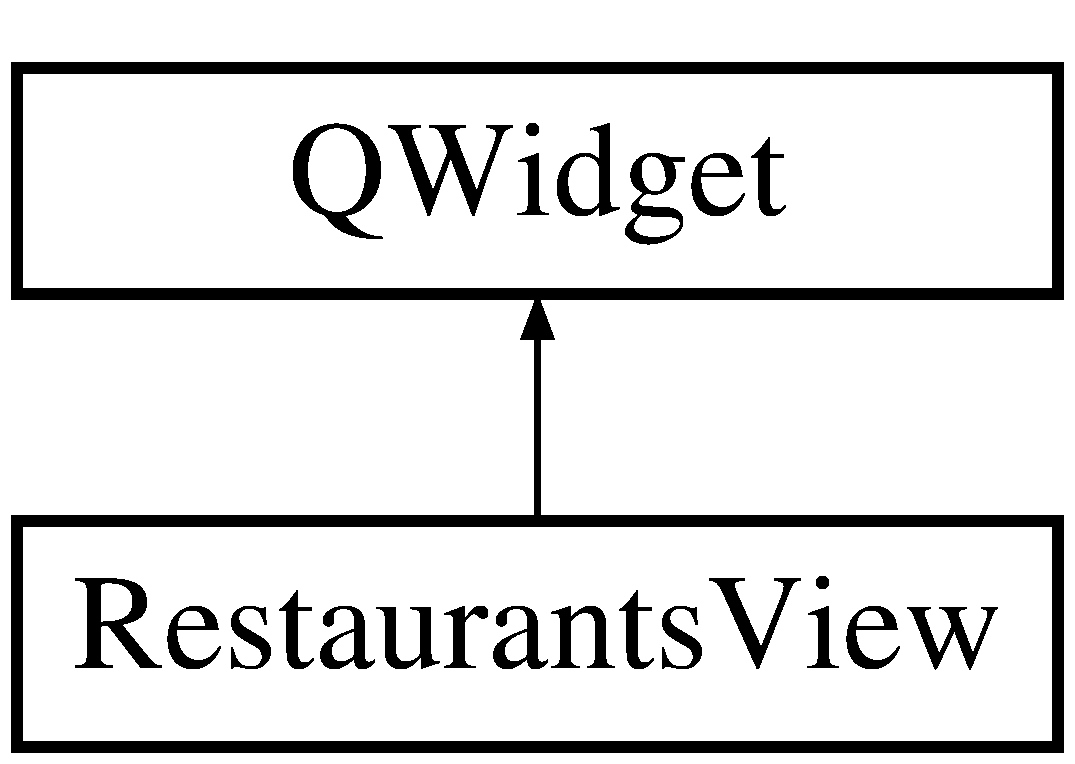
\includegraphics[height=2.000000cm]{classRestaurantsView}
\end{center}
\end{figure}
\subsection*{Public Slots}
\begin{DoxyCompactItemize}
\item 
void \hyperlink{classRestaurantsView_ae5fe4c7bf8970905496fdf55ca4741c6}{reset\-View} ()
\begin{DoxyCompactList}\small\item\em Reset view. \end{DoxyCompactList}\item 
void \hyperlink{classRestaurantsView_a13c38f1c5fef460f6f3bce488857f58c}{reset\-Ui} ()
\begin{DoxyCompactList}\small\item\em Reset all ui in the view. \end{DoxyCompactList}\end{DoxyCompactItemize}
\subsection*{Public Member Functions}
\begin{DoxyCompactItemize}
\item 
\hyperlink{classRestaurantsView_aeba0fdce5e48ca0b103923c6e3456890}{Restaurants\-View} (Q\-Widget $\ast$parent, \hyperlink{classRestaurantDataStore}{Restaurant\-Data\-Store} $\ast$)
\begin{DoxyCompactList}\small\item\em Constructor. \end{DoxyCompactList}\item 
\hyperlink{classRestaurantsView_a176dd3f9964c44886194ce3907f97289}{$\sim$\-Restaurants\-View} ()
\begin{DoxyCompactList}\small\item\em Destructor. \end{DoxyCompactList}\end{DoxyCompactItemize}


\subsection{Detailed Description}
A view that will display all restaurants and their corresponding menu items. 

\subsection{Constructor \& Destructor Documentation}
\hypertarget{classRestaurantsView_aeba0fdce5e48ca0b103923c6e3456890}{\index{Restaurants\-View@{Restaurants\-View}!Restaurants\-View@{Restaurants\-View}}
\index{Restaurants\-View@{Restaurants\-View}!RestaurantsView@{Restaurants\-View}}
\subsubsection[{Restaurants\-View}]{\setlength{\rightskip}{0pt plus 5cm}Restaurants\-View\-::\-Restaurants\-View (
\begin{DoxyParamCaption}
\item[{Q\-Widget $\ast$}]{parent, }
\item[{{\bf Restaurant\-Data\-Store} $\ast$}]{store}
\end{DoxyParamCaption}
)}}\label{classRestaurantsView_aeba0fdce5e48ca0b103923c6e3456890}


Constructor. 

Instantiates the view with list a restaurant and menu list.


\begin{DoxyParams}{Parameters}
{\em parent} & The parent widget that this view will be in \\
\hline
{\em store} & The data store that contains all the data \\
\hline
\end{DoxyParams}
\hypertarget{classRestaurantsView_a176dd3f9964c44886194ce3907f97289}{\index{Restaurants\-View@{Restaurants\-View}!$\sim$\-Restaurants\-View@{$\sim$\-Restaurants\-View}}
\index{$\sim$\-Restaurants\-View@{$\sim$\-Restaurants\-View}!RestaurantsView@{Restaurants\-View}}
\subsubsection[{$\sim$\-Restaurants\-View}]{\setlength{\rightskip}{0pt plus 5cm}Restaurants\-View\-::$\sim$\-Restaurants\-View (
\begin{DoxyParamCaption}
{}
\end{DoxyParamCaption}
)}}\label{classRestaurantsView_a176dd3f9964c44886194ce3907f97289}


Destructor. 

Deletes all dynamically allocated memory. 

\subsection{Member Function Documentation}
\hypertarget{classRestaurantsView_a13c38f1c5fef460f6f3bce488857f58c}{\index{Restaurants\-View@{Restaurants\-View}!reset\-Ui@{reset\-Ui}}
\index{reset\-Ui@{reset\-Ui}!RestaurantsView@{Restaurants\-View}}
\subsubsection[{reset\-Ui}]{\setlength{\rightskip}{0pt plus 5cm}void Restaurants\-View\-::reset\-Ui (
\begin{DoxyParamCaption}
{}
\end{DoxyParamCaption}
)\hspace{0.3cm}{\ttfamily [slot]}}}\label{classRestaurantsView_a13c38f1c5fef460f6f3bce488857f58c}


Reset all ui in the view. 

Reset the restaurant name label. Reload the restaurant list. Clear the menu list. \hypertarget{classRestaurantsView_ae5fe4c7bf8970905496fdf55ca4741c6}{\index{Restaurants\-View@{Restaurants\-View}!reset\-View@{reset\-View}}
\index{reset\-View@{reset\-View}!RestaurantsView@{Restaurants\-View}}
\subsubsection[{reset\-View}]{\setlength{\rightskip}{0pt plus 5cm}void Restaurants\-View\-::reset\-View (
\begin{DoxyParamCaption}
{}
\end{DoxyParamCaption}
)\hspace{0.3cm}{\ttfamily [slot]}}}\label{classRestaurantsView_ae5fe4c7bf8970905496fdf55ca4741c6}


Reset view. 

Resets the view so it looks just like it was when it was created. 

The documentation for this class was generated from the following files\-:\begin{DoxyCompactItemize}
\item 
/home/edt/\-C\-S1\-D/\-C\-S1\-D\-\_\-\-Fast\-\_\-\-Food\-\_\-\-Project/\-Fast\-Food\-Finder/src/views/restaurantsview.\-hpp\item 
/home/edt/\-C\-S1\-D/\-C\-S1\-D\-\_\-\-Fast\-\_\-\-Food\-\_\-\-Project/\-Fast\-Food\-Finder/src/views/restaurantsview.\-cpp\end{DoxyCompactItemize}

\hypertarget{classTrip}{\section{Trip Class Reference}
\label{classTrip}\index{Trip@{Trip}}
}


{\ttfamily \#include $<$Trip.\-hpp$>$}

\subsection*{Public Member Functions}
\begin{DoxyCompactItemize}
\item 
virtual \hyperlink{classTrip_a2376daed3b03469163782ef0d0533d52}{$\sim$\-Trip} ()
\item 
\hyperlink{classTrip_acc40ce84bd727fcf87bca52766d3e32e}{Trip} (int \hyperlink{classUser}{User}, const vector$<$ int $>$ \&Restaurants, float Total\-Distance, const string \&Name)
\item 
\hyperlink{classTrip_a911733e55bacf367b5525c685df4cd39}{Trip} (int Trip\-Num, int \hyperlink{classUser}{User}, const vector$<$ int $>$ \&Restaurants, float Total\-Distance, const string \&Name, bool b\-Trip\-Deleted)
\item 
\hyperlink{classTrip_adc03c8f6d600f0319fe083966210ae70}{Trip} (const \hyperlink{classTrip}{Trip} \&src)
\item 
\hyperlink{classTrip}{Trip} \& \hyperlink{classTrip_a16e1987dd99c6c5650c2f658e4c7e5c7}{operator=} (const \hyperlink{classTrip}{Trip} \&rhs)
\item 
int \hyperlink{classTrip_acdd93f492bafbf08f4e0d60729af1044}{Get\-Number} (void) const 
\item 
const string \& \hyperlink{classTrip_a3590aa8140eba5355e5fc5405ee95bb4}{Get\-Name} (void) const 
\item 
int \hyperlink{classTrip_a6776387c1783c392977b4ed206dbd7f7}{Get\-Creating\-User} (void) const 
\item 
const vector$<$ int $>$ \& \hyperlink{classTrip_a6f64deeab3d0235ff335b74715a3ff0e}{Get\-Restaurants} (void) const 
\item 
float \hyperlink{classTrip_a996654641498d12de7b8b86bf2cfacc2}{Get\-Total\-Distance} (void) const 
\item 
bool \hyperlink{classTrip_ac2f4c16262173e4eef3a9a80d13ddbf9}{Mark\-Deleted} (bool Delete)
\item 
bool \hyperlink{classTrip_acb8e9846f1c211d78191bdf08d1b6c2c}{Is\-Deleted} (void) const 
\item 
bool \hyperlink{classTrip_a68ccf536e61ca8e03082ab8b78769fbd}{Add\-Restaurant} (int \hyperlink{classRestaurant}{Restaurant})
\item 
bool \hyperlink{classTrip_aeb248b2f0083d775c829403681cc27ce}{Print\-As\-Debug} (bool print\-\_\-endl) const 
\end{DoxyCompactItemize}
\subsection*{Friends}
\begin{DoxyCompactItemize}
\item 
\hypertarget{classTrip_a5f322cf906a710abf1da068195287044}{class {\bfseries Trip\-Data\-Store}}\label{classTrip_a5f322cf906a710abf1da068195287044}

\item 
ostream \& \hyperlink{classTrip_a2afdee2004fa7c75dd8fbd878bf9b229}{operator$<$$<$} (ostream \&os, const \hyperlink{classTrip}{Trip} \&trip)
\end{DoxyCompactItemize}


\subsection{Detailed Description}
\hyperlink{classTrip}{Trip} -\/ store information about Trips planned or taken

\begin{DoxyAuthor}{Author}
edt (3/25/19) 
\end{DoxyAuthor}


\subsection{Constructor \& Destructor Documentation}
\hypertarget{classTrip_a2376daed3b03469163782ef0d0533d52}{\index{Trip@{Trip}!$\sim$\-Trip@{$\sim$\-Trip}}
\index{$\sim$\-Trip@{$\sim$\-Trip}!Trip@{Trip}}
\subsubsection[{$\sim$\-Trip}]{\setlength{\rightskip}{0pt plus 5cm}Trip\-::$\sim$\-Trip (
\begin{DoxyParamCaption}
{}
\end{DoxyParamCaption}
)\hspace{0.3cm}{\ttfamily [virtual]}}}\label{classTrip_a2376daed3b03469163782ef0d0533d52}
\hyperlink{classTrip_a2376daed3b03469163782ef0d0533d52}{Trip\-::$\sim$\-Trip} -\/ Destructor

\begin{DoxyAuthor}{Author}
edt (3/25/19) 
\end{DoxyAuthor}
\hypertarget{classTrip_acc40ce84bd727fcf87bca52766d3e32e}{\index{Trip@{Trip}!Trip@{Trip}}
\index{Trip@{Trip}!Trip@{Trip}}
\subsubsection[{Trip}]{\setlength{\rightskip}{0pt plus 5cm}Trip\-::\-Trip (
\begin{DoxyParamCaption}
\item[{int}]{User, }
\item[{const vector$<$ int $>$ \&}]{Restaurants, }
\item[{float}]{Total\-Distance, }
\item[{const string \&}]{Name}
\end{DoxyParamCaption}
)}}\label{classTrip_acc40ce84bd727fcf87bca52766d3e32e}
Trip\-::\-Trip -\/ constructor used when adding trip manually -\/ depricated

\begin{DoxyAuthor}{Author}
edt (3/25/19)
\end{DoxyAuthor}

\begin{DoxyParams}{Parameters}
{\em \hyperlink{classUser}{User}} & -\/ \hyperlink{classUser}{User} planning trip \\
\hline
{\em Restaurants} & -\/ Restaurants on trip \\
\hline
{\em Total\-Distance} & -\/ length of trip in miles \\
\hline
{\em Name} & -\/ Name of \hyperlink{classTrip}{Trip} \\
\hline
\end{DoxyParams}
\hypertarget{classTrip_a911733e55bacf367b5525c685df4cd39}{\index{Trip@{Trip}!Trip@{Trip}}
\index{Trip@{Trip}!Trip@{Trip}}
\subsubsection[{Trip}]{\setlength{\rightskip}{0pt plus 5cm}Trip\-::\-Trip (
\begin{DoxyParamCaption}
\item[{int}]{Trip\-Num, }
\item[{int}]{User, }
\item[{const vector$<$ int $>$ \&}]{Restaurants, }
\item[{float}]{Total\-Distance, }
\item[{const string \&}]{Name, }
\item[{bool}]{b\-Trip\-Deleted}
\end{DoxyParamCaption}
)}}\label{classTrip_a911733e55bacf367b5525c685df4cd39}
Trip\-::\-Trip -\/ Constructor used only by \hyperlink{classTripDataStore}{Trip\-Data\-Store} to load datastore

\begin{DoxyAuthor}{Author}
edt (3/25/19)
\end{DoxyAuthor}

\begin{DoxyParams}{Parameters}
{\em Trip\-Num} & -\/ number \\
\hline
{\em \hyperlink{classUser}{User}} & -\/ creating user \\
\hline
{\em Restaurants} & -\/ restaurants on trip \\
\hline
{\em Total\-Distance} & -\/ distance in miles \\
\hline
{\em Name} & -\/ name of trip \\
\hline
{\em b\-Trip\-Deleted} & -\/ true if deleted -\/ cannot be taken again \\
\hline
\end{DoxyParams}
\hypertarget{classTrip_adc03c8f6d600f0319fe083966210ae70}{\index{Trip@{Trip}!Trip@{Trip}}
\index{Trip@{Trip}!Trip@{Trip}}
\subsubsection[{Trip}]{\setlength{\rightskip}{0pt plus 5cm}Trip\-::\-Trip (
\begin{DoxyParamCaption}
\item[{const {\bf Trip} \&}]{src}
\end{DoxyParamCaption}
)}}\label{classTrip_adc03c8f6d600f0319fe083966210ae70}
Trip\-::\-Trip -\/ Copy constructor

\begin{DoxyAuthor}{Author}
edt (3/25/19)
\end{DoxyAuthor}

\begin{DoxyParams}{Parameters}
{\em src} & -\/ Item to copy \\
\hline
\end{DoxyParams}


\subsection{Member Function Documentation}
\hypertarget{classTrip_a68ccf536e61ca8e03082ab8b78769fbd}{\index{Trip@{Trip}!Add\-Restaurant@{Add\-Restaurant}}
\index{Add\-Restaurant@{Add\-Restaurant}!Trip@{Trip}}
\subsubsection[{Add\-Restaurant}]{\setlength{\rightskip}{0pt plus 5cm}bool Trip\-::\-Add\-Restaurant (
\begin{DoxyParamCaption}
\item[{int}]{Restaurant}
\end{DoxyParamCaption}
)}}\label{classTrip_a68ccf536e61ca8e03082ab8b78769fbd}
\hyperlink{classTrip_a68ccf536e61ca8e03082ab8b78769fbd}{Trip\-::\-Add\-Restaurant} -\/ depricated -\/ use Store\-Trip

\begin{DoxyAuthor}{Author}
edt (3/25/19)
\end{DoxyAuthor}

\begin{DoxyParams}{Parameters}
{\em \hyperlink{classRestaurant}{Restaurant}} & -\/ number of restaurant to add\\
\hline
\end{DoxyParams}
\begin{DoxyReturn}{Returns}
bool -\/ true if added 
\end{DoxyReturn}
\hypertarget{classTrip_a6776387c1783c392977b4ed206dbd7f7}{\index{Trip@{Trip}!Get\-Creating\-User@{Get\-Creating\-User}}
\index{Get\-Creating\-User@{Get\-Creating\-User}!Trip@{Trip}}
\subsubsection[{Get\-Creating\-User}]{\setlength{\rightskip}{0pt plus 5cm}int Trip\-::\-Get\-Creating\-User (
\begin{DoxyParamCaption}
\item[{void}]{}
\end{DoxyParamCaption}
) const}}\label{classTrip_a6776387c1783c392977b4ed206dbd7f7}
\hyperlink{classTrip_a6776387c1783c392977b4ed206dbd7f7}{Trip\-::\-Get\-Creating\-User}

\begin{DoxyAuthor}{Author}
edt (3/25/19)
\end{DoxyAuthor}

\begin{DoxyParams}{Parameters}
{\em void} & \\
\hline
\end{DoxyParams}
\begin{DoxyReturn}{Returns}
int -\/ number of user who planned this trip 
\end{DoxyReturn}
\hypertarget{classTrip_a3590aa8140eba5355e5fc5405ee95bb4}{\index{Trip@{Trip}!Get\-Name@{Get\-Name}}
\index{Get\-Name@{Get\-Name}!Trip@{Trip}}
\subsubsection[{Get\-Name}]{\setlength{\rightskip}{0pt plus 5cm}const string \& Trip\-::\-Get\-Name (
\begin{DoxyParamCaption}
\item[{void}]{}
\end{DoxyParamCaption}
) const}}\label{classTrip_a3590aa8140eba5355e5fc5405ee95bb4}
\hyperlink{classTrip_a3590aa8140eba5355e5fc5405ee95bb4}{Trip\-::\-Get\-Name}

\begin{DoxyAuthor}{Author}
edt (3/25/19)
\end{DoxyAuthor}

\begin{DoxyParams}{Parameters}
{\em void} & \\
\hline
\end{DoxyParams}
\begin{DoxyReturn}{Returns}
const string\& -\/ name of trip 
\end{DoxyReturn}
\hypertarget{classTrip_acdd93f492bafbf08f4e0d60729af1044}{\index{Trip@{Trip}!Get\-Number@{Get\-Number}}
\index{Get\-Number@{Get\-Number}!Trip@{Trip}}
\subsubsection[{Get\-Number}]{\setlength{\rightskip}{0pt plus 5cm}int Trip\-::\-Get\-Number (
\begin{DoxyParamCaption}
\item[{void}]{}
\end{DoxyParamCaption}
) const}}\label{classTrip_acdd93f492bafbf08f4e0d60729af1044}
\hyperlink{classTrip_acdd93f492bafbf08f4e0d60729af1044}{Trip\-::\-Get\-Number}

\begin{DoxyAuthor}{Author}
edt (3/25/19)
\end{DoxyAuthor}

\begin{DoxyParams}{Parameters}
{\em void} & \\
\hline
\end{DoxyParams}
\begin{DoxyReturn}{Returns}
int -\/ name of trip 
\end{DoxyReturn}
\hypertarget{classTrip_a6f64deeab3d0235ff335b74715a3ff0e}{\index{Trip@{Trip}!Get\-Restaurants@{Get\-Restaurants}}
\index{Get\-Restaurants@{Get\-Restaurants}!Trip@{Trip}}
\subsubsection[{Get\-Restaurants}]{\setlength{\rightskip}{0pt plus 5cm}const vector$<$ int $>$ \& Trip\-::\-Get\-Restaurants (
\begin{DoxyParamCaption}
\item[{void}]{}
\end{DoxyParamCaption}
) const}}\label{classTrip_a6f64deeab3d0235ff335b74715a3ff0e}
\hyperlink{classTrip_a6f64deeab3d0235ff335b74715a3ff0e}{Trip\-::\-Get\-Restaurants} -\/ get list of Restaurants to allow taking the trip

\begin{DoxyAuthor}{Author}
edt (3/25/19)
\end{DoxyAuthor}

\begin{DoxyParams}{Parameters}
{\em void} & \\
\hline
\end{DoxyParams}
\begin{DoxyReturn}{Returns}
const vector$<$int$>$\& -\/ vector of ints that are restaurant numbers 
\end{DoxyReturn}
\hypertarget{classTrip_a996654641498d12de7b8b86bf2cfacc2}{\index{Trip@{Trip}!Get\-Total\-Distance@{Get\-Total\-Distance}}
\index{Get\-Total\-Distance@{Get\-Total\-Distance}!Trip@{Trip}}
\subsubsection[{Get\-Total\-Distance}]{\setlength{\rightskip}{0pt plus 5cm}float Trip\-::\-Get\-Total\-Distance (
\begin{DoxyParamCaption}
\item[{void}]{}
\end{DoxyParamCaption}
) const}}\label{classTrip_a996654641498d12de7b8b86bf2cfacc2}
\hyperlink{classTrip_a996654641498d12de7b8b86bf2cfacc2}{Trip\-::\-Get\-Total\-Distance}

\begin{DoxyAuthor}{Author}
edt (3/25/19)
\end{DoxyAuthor}

\begin{DoxyParams}{Parameters}
{\em void} & \\
\hline
\end{DoxyParams}
\begin{DoxyReturn}{Returns}
float -\/ distance in miles for entire trip 
\end{DoxyReturn}
\hypertarget{classTrip_acb8e9846f1c211d78191bdf08d1b6c2c}{\index{Trip@{Trip}!Is\-Deleted@{Is\-Deleted}}
\index{Is\-Deleted@{Is\-Deleted}!Trip@{Trip}}
\subsubsection[{Is\-Deleted}]{\setlength{\rightskip}{0pt plus 5cm}bool Trip\-::\-Is\-Deleted (
\begin{DoxyParamCaption}
\item[{void}]{}
\end{DoxyParamCaption}
) const}}\label{classTrip_acb8e9846f1c211d78191bdf08d1b6c2c}
\hyperlink{classTrip_acb8e9846f1c211d78191bdf08d1b6c2c}{Trip\-::\-Is\-Deleted}

\begin{DoxyAuthor}{Author}
edt (3/25/19)
\end{DoxyAuthor}

\begin{DoxyParams}{Parameters}
{\em void} & \\
\hline
\end{DoxyParams}
\begin{DoxyReturn}{Returns}
bool -\/ true if trip is deleted and should not be taken again 
\end{DoxyReturn}
\hypertarget{classTrip_ac2f4c16262173e4eef3a9a80d13ddbf9}{\index{Trip@{Trip}!Mark\-Deleted@{Mark\-Deleted}}
\index{Mark\-Deleted@{Mark\-Deleted}!Trip@{Trip}}
\subsubsection[{Mark\-Deleted}]{\setlength{\rightskip}{0pt plus 5cm}bool Trip\-::\-Mark\-Deleted (
\begin{DoxyParamCaption}
\item[{bool}]{Delete}
\end{DoxyParamCaption}
)}}\label{classTrip_ac2f4c16262173e4eef3a9a80d13ddbf9}
\hyperlink{classTrip_ac2f4c16262173e4eef3a9a80d13ddbf9}{Trip\-::\-Mark\-Deleted}

\begin{DoxyAuthor}{Author}
edt (3/25/19)
\end{DoxyAuthor}

\begin{DoxyParams}{Parameters}
{\em Delete} & -\/ true if trip is deleted\\
\hline
\end{DoxyParams}
\begin{DoxyReturn}{Returns}
bool -\/ true if trip is deleted and should not be taken again 
\end{DoxyReturn}
\hypertarget{classTrip_a16e1987dd99c6c5650c2f658e4c7e5c7}{\index{Trip@{Trip}!operator=@{operator=}}
\index{operator=@{operator=}!Trip@{Trip}}
\subsubsection[{operator=}]{\setlength{\rightskip}{0pt plus 5cm}{\bf Trip} \& Trip\-::operator= (
\begin{DoxyParamCaption}
\item[{const {\bf Trip} \&}]{rhs}
\end{DoxyParamCaption}
)}}\label{classTrip_a16e1987dd99c6c5650c2f658e4c7e5c7}
\hyperlink{classTrip_a16e1987dd99c6c5650c2f658e4c7e5c7}{Trip\-::operator=}

\begin{DoxyAuthor}{Author}
edt (3/25/19)
\end{DoxyAuthor}

\begin{DoxyParams}{Parameters}
{\em rhs} & -\/ Item to copy\\
\hline
\end{DoxyParams}
\begin{DoxyReturn}{Returns}
\hyperlink{classTrip}{Trip}\& 
\end{DoxyReturn}
\hypertarget{classTrip_aeb248b2f0083d775c829403681cc27ce}{\index{Trip@{Trip}!Print\-As\-Debug@{Print\-As\-Debug}}
\index{Print\-As\-Debug@{Print\-As\-Debug}!Trip@{Trip}}
\subsubsection[{Print\-As\-Debug}]{\setlength{\rightskip}{0pt plus 5cm}bool Trip\-::\-Print\-As\-Debug (
\begin{DoxyParamCaption}
\item[{bool}]{print\-\_\-endl}
\end{DoxyParamCaption}
) const}}\label{classTrip_aeb248b2f0083d775c829403681cc27ce}
print the value of the object for external display

\begin{DoxyAuthor}{Author}
edt (2/7/18)
\end{DoxyAuthor}

\begin{DoxyParams}{Parameters}
{\em print\-\_\-endl} & -\/ print end of line between each field\\
\hline
\end{DoxyParams}
\begin{DoxyReturn}{Returns}
bool -\/ true if no errors 
\end{DoxyReturn}


\subsection{Friends And Related Function Documentation}
\hypertarget{classTrip_a2afdee2004fa7c75dd8fbd878bf9b229}{\index{Trip@{Trip}!operator$<$$<$@{operator$<$$<$}}
\index{operator$<$$<$@{operator$<$$<$}!Trip@{Trip}}
\subsubsection[{operator$<$$<$}]{\setlength{\rightskip}{0pt plus 5cm}ostream\& operator$<$$<$ (
\begin{DoxyParamCaption}
\item[{ostream \&}]{os, }
\item[{const {\bf Trip} \&}]{trip}
\end{DoxyParamCaption}
)\hspace{0.3cm}{\ttfamily [friend]}}}\label{classTrip_a2afdee2004fa7c75dd8fbd878bf9b229}
Overloaded operator $<$$<$ to print the contents of an \hyperlink{classTrip}{Trip} object

\begin{DoxyAuthor}{Author}
edt (2/7/18)
\end{DoxyAuthor}

\begin{DoxyParams}{Parameters}
{\em os} & -\/ output stream being processed \\
\hline
{\em trip} & -\/ object to print\\
\hline
\end{DoxyParams}
\begin{DoxyReturn}{Returns}
ostream\&-\/ output stream being processed 
\end{DoxyReturn}


The documentation for this class was generated from the following files\-:\begin{DoxyCompactItemize}
\item 
/home/edt/\-C\-S1\-D/\-C\-S1\-D\-\_\-\-Fast\-\_\-\-Food\-\_\-\-Project/\-Fast\-Food\-Finder/src/datastore/Trip.\-hpp\item 
/home/edt/\-C\-S1\-D/\-C\-S1\-D\-\_\-\-Fast\-\_\-\-Food\-\_\-\-Project/\-Fast\-Food\-Finder/src/datastore/Trip.\-cpp\end{DoxyCompactItemize}

\hypertarget{classTripDataStore}{\section{Trip\-Data\-Store Class Reference}
\label{classTripDataStore}\index{Trip\-Data\-Store@{Trip\-Data\-Store}}
}


{\ttfamily \#include $<$Trip\-Data\-Store.\-hpp$>$}

\subsection*{Public Member Functions}
\begin{DoxyCompactItemize}
\item 
\hyperlink{classTripDataStore_a6ecb3b38f615cdf3a95699b75e070f64}{Trip\-Data\-Store} ()
\item 
virtual \hyperlink{classTripDataStore_abcc0808ffac99fce3d20fec2e6b037db}{$\sim$\-Trip\-Data\-Store} ()
\item 
void \hyperlink{classTripDataStore_a3e0428a62b180370acca3cef17236a13}{print\-As\-Debug} (bool printeol, bool printcontent) const 
\item 
void \hyperlink{classTripDataStore_a6b04d48e105f786d28a6b1c237d0d6c7}{load} (const string path)
\item 
void \hyperlink{classTripDataStore_ac694428dda496c811b1e46a2b206d0cd}{save} (const string path)
\item 
int \hyperlink{classTripDataStore_a45a7c93b2899cf0b7bf070324d686c36}{Store\-Trip} (const string \&Trip\-Name, const vector$<$ int $>$ Restaurants\-Selectedby\-User, \hyperlink{classRestaurantDataStore}{Restaurant\-Data\-Store} \&Rest\-St, \hyperlink{classUser}{User} \&\hyperlink{classUser}{User}, bool Startat\-Saddleback)
\item 
int \hyperlink{classTripDataStore_aef773f76a25496d624c8f7443ab393bc}{Store\-Trip\-Num\-Rest} (const string \&Trip\-Name, int Starting\-Rest\-Num, int Numto\-Visit, \hyperlink{classRestaurantDataStore}{Restaurant\-Data\-Store} \&Rest\-St, \hyperlink{classUser}{User} \&\hyperlink{classUser}{User})
\item 
\hyperlink{classTrip}{Trip} \& \hyperlink{classTripDataStore_a1326494915eee638e4eedbdd6bb0c09b}{Findby\-Number} (int Number)
\end{DoxyCompactItemize}
\subsection*{Public Attributes}
\begin{DoxyCompactItemize}
\item 
\hypertarget{classTripDataStore_a75cb59c927937a86ba9ddeb304a1e4f5}{\hyperlink{classnsMyDblLinkList_1_1MyDblLinkList}{My\-Dbl\-Link\-List}$<$ \hyperlink{classTrip}{Trip} $>$ {\bfseries list}}\label{classTripDataStore_a75cb59c927937a86ba9ddeb304a1e4f5}

\end{DoxyCompactItemize}


\subsection{Detailed Description}
\hyperlink{classTripDataStore}{Trip\-Data\-Store} -\/ internal storage for \hyperlink{classTrip}{Trip} objects

\begin{DoxyAuthor}{Author}
edt (3/25/19) 
\end{DoxyAuthor}


\subsection{Constructor \& Destructor Documentation}
\hypertarget{classTripDataStore_a6ecb3b38f615cdf3a95699b75e070f64}{\index{Trip\-Data\-Store@{Trip\-Data\-Store}!Trip\-Data\-Store@{Trip\-Data\-Store}}
\index{Trip\-Data\-Store@{Trip\-Data\-Store}!TripDataStore@{Trip\-Data\-Store}}
\subsubsection[{Trip\-Data\-Store}]{\setlength{\rightskip}{0pt plus 5cm}Trip\-Data\-Store\-::\-Trip\-Data\-Store (
\begin{DoxyParamCaption}
{}
\end{DoxyParamCaption}
)}}\label{classTripDataStore_a6ecb3b38f615cdf3a95699b75e070f64}
\hyperlink{classTripDataStore_a6ecb3b38f615cdf3a95699b75e070f64}{Trip\-Data\-Store\-::\-Trip\-Data\-Store} -\/ Default Constructor

\begin{DoxyAuthor}{Author}
edt (3/25/19) 
\end{DoxyAuthor}
\hypertarget{classTripDataStore_abcc0808ffac99fce3d20fec2e6b037db}{\index{Trip\-Data\-Store@{Trip\-Data\-Store}!$\sim$\-Trip\-Data\-Store@{$\sim$\-Trip\-Data\-Store}}
\index{$\sim$\-Trip\-Data\-Store@{$\sim$\-Trip\-Data\-Store}!TripDataStore@{Trip\-Data\-Store}}
\subsubsection[{$\sim$\-Trip\-Data\-Store}]{\setlength{\rightskip}{0pt plus 5cm}Trip\-Data\-Store\-::$\sim$\-Trip\-Data\-Store (
\begin{DoxyParamCaption}
{}
\end{DoxyParamCaption}
)\hspace{0.3cm}{\ttfamily [virtual]}}}\label{classTripDataStore_abcc0808ffac99fce3d20fec2e6b037db}
\hyperlink{classTripDataStore_abcc0808ffac99fce3d20fec2e6b037db}{Trip\-Data\-Store\-::$\sim$\-Trip\-Data\-Store} -\/ Destructor

\begin{DoxyAuthor}{Author}
edt (3/25/19) 
\end{DoxyAuthor}


\subsection{Member Function Documentation}
\hypertarget{classTripDataStore_a1326494915eee638e4eedbdd6bb0c09b}{\index{Trip\-Data\-Store@{Trip\-Data\-Store}!Findby\-Number@{Findby\-Number}}
\index{Findby\-Number@{Findby\-Number}!TripDataStore@{Trip\-Data\-Store}}
\subsubsection[{Findby\-Number}]{\setlength{\rightskip}{0pt plus 5cm}{\bf Trip} \& Trip\-Data\-Store\-::\-Findby\-Number (
\begin{DoxyParamCaption}
\item[{int}]{Number}
\end{DoxyParamCaption}
)}}\label{classTripDataStore_a1326494915eee638e4eedbdd6bb0c09b}
\hyperlink{classTripDataStore_a1326494915eee638e4eedbdd6bb0c09b}{Trip\-Data\-Store\-::\-Findby\-Number}

\begin{DoxyAuthor}{Author}
edt (3/25/19)
\end{DoxyAuthor}

\begin{DoxyParams}{Parameters}
{\em Number} & -\/ number of trip to locate\\
\hline
\end{DoxyParams}
\begin{DoxyReturn}{Returns}
\hyperlink{classTrip}{Trip}\& -\/ pointer to trip specified or N\-U\-L\-L if not present 
\end{DoxyReturn}
\hypertarget{classTripDataStore_a6b04d48e105f786d28a6b1c237d0d6c7}{\index{Trip\-Data\-Store@{Trip\-Data\-Store}!load@{load}}
\index{load@{load}!TripDataStore@{Trip\-Data\-Store}}
\subsubsection[{load}]{\setlength{\rightskip}{0pt plus 5cm}void Trip\-Data\-Store\-::load (
\begin{DoxyParamCaption}
\item[{const string}]{path}
\end{DoxyParamCaption}
)}}\label{classTripDataStore_a6b04d48e105f786d28a6b1c237d0d6c7}
\hyperlink{classTripDataStore_a6b04d48e105f786d28a6b1c237d0d6c7}{Trip\-Data\-Store\-::load} -\/ load items from external file into datastore

\begin{DoxyAuthor}{Author}
edt (3/25/19)
\end{DoxyAuthor}

\begin{DoxyParams}{Parameters}
{\em path} & -\/ location of external C\-S\-V file to load \\
\hline
\end{DoxyParams}
\hypertarget{classTripDataStore_a3e0428a62b180370acca3cef17236a13}{\index{Trip\-Data\-Store@{Trip\-Data\-Store}!print\-As\-Debug@{print\-As\-Debug}}
\index{print\-As\-Debug@{print\-As\-Debug}!TripDataStore@{Trip\-Data\-Store}}
\subsubsection[{print\-As\-Debug}]{\setlength{\rightskip}{0pt plus 5cm}void Trip\-Data\-Store\-::print\-As\-Debug (
\begin{DoxyParamCaption}
\item[{bool}]{printeol, }
\item[{bool}]{printcontent}
\end{DoxyParamCaption}
) const}}\label{classTripDataStore_a3e0428a62b180370acca3cef17236a13}
\hyperlink{classTripDataStore_a3e0428a62b180370acca3cef17236a13}{Trip\-Data\-Store\-::print\-As\-Debug} helper function to print internal state of all objects in datastore

\begin{DoxyAuthor}{Author}
edt (3/25/19)
\end{DoxyAuthor}

\begin{DoxyParams}{Parameters}
{\em printeol} & -\/ print end of line after each element \\
\hline
{\em printcontent-\/} & print interanl state of each \hyperlink{classTrip}{Trip} \\
\hline
\end{DoxyParams}
\hypertarget{classTripDataStore_ac694428dda496c811b1e46a2b206d0cd}{\index{Trip\-Data\-Store@{Trip\-Data\-Store}!save@{save}}
\index{save@{save}!TripDataStore@{Trip\-Data\-Store}}
\subsubsection[{save}]{\setlength{\rightskip}{0pt plus 5cm}void Trip\-Data\-Store\-::save (
\begin{DoxyParamCaption}
\item[{const string}]{path}
\end{DoxyParamCaption}
)}}\label{classTripDataStore_ac694428dda496c811b1e46a2b206d0cd}
\hyperlink{classTripDataStore_ac694428dda496c811b1e46a2b206d0cd}{Trip\-Data\-Store\-::save} -\/ save datastore to external C\-S\-V file

\begin{DoxyAuthor}{Author}
edt (3/25/19)
\end{DoxyAuthor}

\begin{DoxyParams}{Parameters}
{\em path} & -\/ path to external C\-S\-V file (will be overwitten) \\
\hline
\end{DoxyParams}
\hypertarget{classTripDataStore_a45a7c93b2899cf0b7bf070324d686c36}{\index{Trip\-Data\-Store@{Trip\-Data\-Store}!Store\-Trip@{Store\-Trip}}
\index{Store\-Trip@{Store\-Trip}!TripDataStore@{Trip\-Data\-Store}}
\subsubsection[{Store\-Trip}]{\setlength{\rightskip}{0pt plus 5cm}int Trip\-Data\-Store\-::\-Store\-Trip (
\begin{DoxyParamCaption}
\item[{const string \&}]{Trip\-Name, }
\item[{const vector$<$ int $>$}]{Restaurants\-Selectedby\-User, }
\item[{{\bf Restaurant\-Data\-Store} \&}]{Rest\-St, }
\item[{{\bf User} \&}]{User, }
\item[{bool}]{Startat\-Saddleback}
\end{DoxyParamCaption}
)}}\label{classTripDataStore_a45a7c93b2899cf0b7bf070324d686c36}
\hyperlink{classTripDataStore_a45a7c93b2899cf0b7bf070324d686c36}{Trip\-Data\-Store\-::\-Store\-Trip} -\/ create \hyperlink{classTrip}{Trip} from planning data entered by user sorts the selected restaurants by shortest distance to next restaurant

\begin{DoxyAuthor}{Author}
edt (3/25/19)
\end{DoxyAuthor}

\begin{DoxyParams}{Parameters}
{\em Trip\-Name} & -\/ name of trip \\
\hline
{\em Restaurants\-Selectedby\-User} & -\/ vector of ints that represent restaurants \\
\hline
{\em Rest\-St} & -\/ pointer to \hyperlink{classRestaurantDataStore}{Restaurant\-Data\-Store} \\
\hline
{\em \hyperlink{classUser}{User}} & -\/ pointer to creating user \\
\hline
{\em Startat\-Saddleback} & -\/ true if trip originates at Saddleback\\
\hline
\end{DoxyParams}
\begin{DoxyReturn}{Returns}
int -\/ Number assigned to this trip 
\end{DoxyReturn}
\hypertarget{classTripDataStore_aef773f76a25496d624c8f7443ab393bc}{\index{Trip\-Data\-Store@{Trip\-Data\-Store}!Store\-Trip\-Num\-Rest@{Store\-Trip\-Num\-Rest}}
\index{Store\-Trip\-Num\-Rest@{Store\-Trip\-Num\-Rest}!TripDataStore@{Trip\-Data\-Store}}
\subsubsection[{Store\-Trip\-Num\-Rest}]{\setlength{\rightskip}{0pt plus 5cm}int Trip\-Data\-Store\-::\-Store\-Trip\-Num\-Rest (
\begin{DoxyParamCaption}
\item[{const string \&}]{Trip\-Name, }
\item[{int}]{Starting\-Rest\-Num, }
\item[{int}]{Numto\-Visit, }
\item[{{\bf Restaurant\-Data\-Store} \&}]{Rest\-St, }
\item[{{\bf User} \&}]{User}
\end{DoxyParamCaption}
)}}\label{classTripDataStore_aef773f76a25496d624c8f7443ab393bc}
\hyperlink{classTripDataStore_aef773f76a25496d624c8f7443ab393bc}{Trip\-Data\-Store\-::\-Store\-Trip\-Num\-Rest} create \hyperlink{classTrip}{Trip} from planning data entered by user sorts the selected restaurants by shortest distance to next restaurant

\begin{DoxyAuthor}{Author}
edt (3/25/19)
\end{DoxyAuthor}

\begin{DoxyParams}{Parameters}
{\em Trip\-Name} & -\/ name of trip \\
\hline
{\em Starting\-Rest\-Num} & -\/ starting location for trip, 0 if Saddleback \\
\hline
{\em Numto\-Visit} & -\/ number of restaurants to visit \\
\hline
{\em Rest\-St} & -\/ pointer to \hyperlink{classRestaurantDataStore}{Restaurant\-Data\-Store} \\
\hline
{\em \hyperlink{classUser}{User}} & -\/ pointer to creating user\\
\hline
\end{DoxyParams}
\begin{DoxyReturn}{Returns}
int -\/ Number assigned to this trip 
\end{DoxyReturn}


The documentation for this class was generated from the following files\-:\begin{DoxyCompactItemize}
\item 
/home/edt/\-C\-S1\-D/\-C\-S1\-D\-\_\-\-Fast\-\_\-\-Food\-\_\-\-Project/\-Fast\-Food\-Finder/src/datastore/Trip\-Data\-Store.\-hpp\item 
/home/edt/\-C\-S1\-D/\-C\-S1\-D\-\_\-\-Fast\-\_\-\-Food\-\_\-\-Project/\-Fast\-Food\-Finder/src/datastore/Trip\-Data\-Store.\-cpp\end{DoxyCompactItemize}

\hypertarget{classUser}{\section{User Class Reference}
\label{classUser}\index{User@{User}}
}


{\ttfamily \#include $<$User.\-hpp$>$}

\subsection*{Public Member Functions}
\begin{DoxyCompactItemize}
\item 
\hyperlink{classUser_a6eac4d795eb00dd593420fe958e4c065}{User} (const string \&Name, const string \&Password)
\item 
virtual \hyperlink{classUser_ac00b72ad64eb4149f7b21b9f5468c2b2}{$\sim$\-User} ()
\item 
\hyperlink{classUser_afaee5de8c92bac691705144d524c0603}{User} (const \hyperlink{classUser}{User} \&src)
\item 
\hyperlink{classUser}{User} \& \hyperlink{classUser_a6a108fd294b05801932c988e500960ed}{operator=} (const \hyperlink{classUser}{User} \&src)
\item 
const int \hyperlink{classUser_ac4863972c5f3e83492ed6aef96831823}{Get\-Number} (void) const 
\item 
const string \& \hyperlink{classUser_add35a9560dfdffbfa68131659cb73042}{Get\-Name} (void) const 
\item 
const string \& \hyperlink{classUser_a6d4df29ccff3066db39c8e382dc35e25}{Get\-Hashed\-Passwd} (void) const 
\item 
bool \hyperlink{classUser_aa6dde0521a45afe94251ab635c2c7011}{Mark\-Deleted} (bool Delete)
\item 
bool \hyperlink{classUser_a87987969d79e97bc15fdd17179a2a783}{Is\-Deleted} (void) const 
\item 
bool \hyperlink{classUser_a0efba1a031faf9ce8626d705fc70f053}{Mark\-Admin} (bool Admin)
\item 
bool \hyperlink{classUser_ad24d48713d03bf244af83e9780397077}{Is\-Admin} (void) const 
\item 
bool \hyperlink{classUser_a4deef20946b4e92147c02b855a5c31b9}{Mark\-Blocked} (bool Block)
\item 
bool \hyperlink{classUser_a5f04d5bbe4e4b77930bcdb127fc07b51}{Is\-Blocked} (void) const 
\item 
float \hyperlink{classUser_a662c053f774423b975955744f06044ad}{Purchase} (float Purchase\-Amount)
\item 
void \hyperlink{classUser_abe5567c17840f6b017449fd03778109f}{Add\-Trip} (int \hyperlink{classTrip}{Trip})
\item 
const vector$<$ int $>$ \& \hyperlink{classUser_ad18180f581f680eece112ce2500173f4}{Get\-Trips} (void) const 
\item 
float \hyperlink{classUser_a911545fcb63f3e7c0cb23a750906f0a4}{Get\-Total\-Purchase} (void) const 
\item 
bool \hyperlink{classUser_ad2dacdc322f613dd5f409d346677ebef}{operator$<$} (\hyperlink{classUser}{User} \&rhs)
\end{DoxyCompactItemize}
\subsection*{Friends}
\begin{DoxyCompactItemize}
\item 
\hypertarget{classUser_a39199a48b6b45757febce5a02120d628}{class {\bfseries User\-Data\-Store}}\label{classUser_a39199a48b6b45757febce5a02120d628}

\item 
ostream \& \hyperlink{classUser_ac22edd304277826206d806856a2fa39f}{operator$<$$<$} (ostream \&os, const \hyperlink{classUser}{User} \&user)
\end{DoxyCompactItemize}


\subsection{Detailed Description}
Stores \hyperlink{classUser}{User} data and provides accessors/mutators

\begin{DoxyAuthor}{Author}
edt (3/25/19) 
\end{DoxyAuthor}


\subsection{Constructor \& Destructor Documentation}
\hypertarget{classUser_a6eac4d795eb00dd593420fe958e4c065}{\index{User@{User}!User@{User}}
\index{User@{User}!User@{User}}
\subsubsection[{User}]{\setlength{\rightskip}{0pt plus 5cm}User\-::\-User (
\begin{DoxyParamCaption}
\item[{const string \&}]{Name, }
\item[{const string \&}]{Password}
\end{DoxyParamCaption}
)}}\label{classUser_a6eac4d795eb00dd593420fe958e4c065}
User\-::\-User -\/ create a new user

\begin{DoxyAuthor}{Author}
edt (3/25/19)
\end{DoxyAuthor}

\begin{DoxyParams}{Parameters}
{\em Name} & -\/ user name \\
\hline
{\em Password} & -\/ string representing hashed password \\
\hline
\end{DoxyParams}
\hypertarget{classUser_ac00b72ad64eb4149f7b21b9f5468c2b2}{\index{User@{User}!$\sim$\-User@{$\sim$\-User}}
\index{$\sim$\-User@{$\sim$\-User}!User@{User}}
\subsubsection[{$\sim$\-User}]{\setlength{\rightskip}{0pt plus 5cm}User\-::$\sim$\-User (
\begin{DoxyParamCaption}
{}
\end{DoxyParamCaption}
)\hspace{0.3cm}{\ttfamily [virtual]}}}\label{classUser_ac00b72ad64eb4149f7b21b9f5468c2b2}
\hyperlink{classUser_ac00b72ad64eb4149f7b21b9f5468c2b2}{User\-::$\sim$\-User} -\/ Destructor

\begin{DoxyAuthor}{Author}
edt (3/25/19) 
\end{DoxyAuthor}
\hypertarget{classUser_afaee5de8c92bac691705144d524c0603}{\index{User@{User}!User@{User}}
\index{User@{User}!User@{User}}
\subsubsection[{User}]{\setlength{\rightskip}{0pt plus 5cm}User\-::\-User (
\begin{DoxyParamCaption}
\item[{const {\bf User} \&}]{src}
\end{DoxyParamCaption}
)}}\label{classUser_afaee5de8c92bac691705144d524c0603}
User\-::\-User -\/ copy constructor

\begin{DoxyAuthor}{Author}
edt (3/25/19)
\end{DoxyAuthor}

\begin{DoxyParams}{Parameters}
{\em src} & -\/ \hyperlink{classUser}{User} to copy \\
\hline
\end{DoxyParams}


\subsection{Member Function Documentation}
\hypertarget{classUser_abe5567c17840f6b017449fd03778109f}{\index{User@{User}!Add\-Trip@{Add\-Trip}}
\index{Add\-Trip@{Add\-Trip}!User@{User}}
\subsubsection[{Add\-Trip}]{\setlength{\rightskip}{0pt plus 5cm}void User\-::\-Add\-Trip (
\begin{DoxyParamCaption}
\item[{int}]{Trip}
\end{DoxyParamCaption}
)}}\label{classUser_abe5567c17840f6b017449fd03778109f}
\hyperlink{classUser_abe5567c17840f6b017449fd03778109f}{User\-::\-Add\-Trip} -\/ depricated -\/ Use Store\-Trip

\begin{DoxyAuthor}{Author}
edt (3/25/19)
\end{DoxyAuthor}

\begin{DoxyParams}{Parameters}
{\em \hyperlink{classTrip}{Trip}} & -\/ trip number planned \\
\hline
\end{DoxyParams}
\hypertarget{classUser_a6d4df29ccff3066db39c8e382dc35e25}{\index{User@{User}!Get\-Hashed\-Passwd@{Get\-Hashed\-Passwd}}
\index{Get\-Hashed\-Passwd@{Get\-Hashed\-Passwd}!User@{User}}
\subsubsection[{Get\-Hashed\-Passwd}]{\setlength{\rightskip}{0pt plus 5cm}const string \& User\-::\-Get\-Hashed\-Passwd (
\begin{DoxyParamCaption}
\item[{void}]{}
\end{DoxyParamCaption}
) const}}\label{classUser_a6d4df29ccff3066db39c8e382dc35e25}
\hyperlink{classUser_a6d4df29ccff3066db39c8e382dc35e25}{User\-::\-Get\-Hashed\-Passwd}

\begin{DoxyAuthor}{Author}
edt (3/25/19)
\end{DoxyAuthor}

\begin{DoxyParams}{Parameters}
{\em void} & \\
\hline
\end{DoxyParams}
\begin{DoxyReturn}{Returns}
const string\& -\/ string representing hashed password 
\end{DoxyReturn}
\hypertarget{classUser_add35a9560dfdffbfa68131659cb73042}{\index{User@{User}!Get\-Name@{Get\-Name}}
\index{Get\-Name@{Get\-Name}!User@{User}}
\subsubsection[{Get\-Name}]{\setlength{\rightskip}{0pt plus 5cm}const string \& User\-::\-Get\-Name (
\begin{DoxyParamCaption}
\item[{void}]{}
\end{DoxyParamCaption}
) const}}\label{classUser_add35a9560dfdffbfa68131659cb73042}
\&\hyperlink{classUser_add35a9560dfdffbfa68131659cb73042}{User\-::\-Get\-Name}

\begin{DoxyAuthor}{Author}
edt (3/25/19)
\end{DoxyAuthor}

\begin{DoxyParams}{Parameters}
{\em void} & \\
\hline
\end{DoxyParams}
\begin{DoxyReturn}{Returns}
const string\& -\/ user name 
\end{DoxyReturn}
\hypertarget{classUser_ac4863972c5f3e83492ed6aef96831823}{\index{User@{User}!Get\-Number@{Get\-Number}}
\index{Get\-Number@{Get\-Number}!User@{User}}
\subsubsection[{Get\-Number}]{\setlength{\rightskip}{0pt plus 5cm}const int User\-::\-Get\-Number (
\begin{DoxyParamCaption}
\item[{void}]{}
\end{DoxyParamCaption}
) const}}\label{classUser_ac4863972c5f3e83492ed6aef96831823}
\hyperlink{classUser_ac4863972c5f3e83492ed6aef96831823}{User\-::\-Get\-Number}

\begin{DoxyAuthor}{Author}
edt (3/25/19)
\end{DoxyAuthor}

\begin{DoxyParams}{Parameters}
{\em void} & \\
\hline
\end{DoxyParams}
\begin{DoxyReturn}{Returns}
const int -\/ user number 
\end{DoxyReturn}
\hypertarget{classUser_a911545fcb63f3e7c0cb23a750906f0a4}{\index{User@{User}!Get\-Total\-Purchase@{Get\-Total\-Purchase}}
\index{Get\-Total\-Purchase@{Get\-Total\-Purchase}!User@{User}}
\subsubsection[{Get\-Total\-Purchase}]{\setlength{\rightskip}{0pt plus 5cm}float User\-::\-Get\-Total\-Purchase (
\begin{DoxyParamCaption}
\item[{void}]{}
\end{DoxyParamCaption}
) const}}\label{classUser_a911545fcb63f3e7c0cb23a750906f0a4}
\hyperlink{classUser_a911545fcb63f3e7c0cb23a750906f0a4}{User\-::\-Get\-Total\-Purchase}

\begin{DoxyAuthor}{Author}
edt (3/25/19)
\end{DoxyAuthor}

\begin{DoxyParams}{Parameters}
{\em void} & \\
\hline
\end{DoxyParams}
\begin{DoxyReturn}{Returns}
float -\/ total amount purchased on all trips 
\end{DoxyReturn}
\hypertarget{classUser_ad18180f581f680eece112ce2500173f4}{\index{User@{User}!Get\-Trips@{Get\-Trips}}
\index{Get\-Trips@{Get\-Trips}!User@{User}}
\subsubsection[{Get\-Trips}]{\setlength{\rightskip}{0pt plus 5cm}const vector$<$ int $>$ \& User\-::\-Get\-Trips (
\begin{DoxyParamCaption}
\item[{void}]{}
\end{DoxyParamCaption}
) const}}\label{classUser_ad18180f581f680eece112ce2500173f4}
\hyperlink{classUser_ad18180f581f680eece112ce2500173f4}{User\-::\-Get\-Trips} -\/ list trips planned by this user

\begin{DoxyAuthor}{Author}
edt (3/25/19)
\end{DoxyAuthor}

\begin{DoxyParams}{Parameters}
{\em void} & \\
\hline
\end{DoxyParams}
\begin{DoxyReturn}{Returns}
const vector$<$int$>$\& -\/ trips planned by this user 
\end{DoxyReturn}
\hypertarget{classUser_ad24d48713d03bf244af83e9780397077}{\index{User@{User}!Is\-Admin@{Is\-Admin}}
\index{Is\-Admin@{Is\-Admin}!User@{User}}
\subsubsection[{Is\-Admin}]{\setlength{\rightskip}{0pt plus 5cm}bool User\-::\-Is\-Admin (
\begin{DoxyParamCaption}
\item[{void}]{}
\end{DoxyParamCaption}
) const}}\label{classUser_ad24d48713d03bf244af83e9780397077}
\hyperlink{classUser_ad24d48713d03bf244af83e9780397077}{User\-::\-Is\-Admin}

\begin{DoxyAuthor}{Author}
edt (3/25/19)
\end{DoxyAuthor}

\begin{DoxyParams}{Parameters}
{\em void} & \\
\hline
\end{DoxyParams}
\begin{DoxyReturn}{Returns}
bool -\/ true if user is an Administrator 
\end{DoxyReturn}
\hypertarget{classUser_a5f04d5bbe4e4b77930bcdb127fc07b51}{\index{User@{User}!Is\-Blocked@{Is\-Blocked}}
\index{Is\-Blocked@{Is\-Blocked}!User@{User}}
\subsubsection[{Is\-Blocked}]{\setlength{\rightskip}{0pt plus 5cm}bool User\-::\-Is\-Blocked (
\begin{DoxyParamCaption}
\item[{void}]{}
\end{DoxyParamCaption}
) const}}\label{classUser_a5f04d5bbe4e4b77930bcdb127fc07b51}
\hyperlink{classUser_a5f04d5bbe4e4b77930bcdb127fc07b51}{User\-::\-Is\-Blocked}

\begin{DoxyAuthor}{Author}
edt (3/25/19)
\end{DoxyAuthor}

\begin{DoxyParams}{Parameters}
{\em void} & \\
\hline
\end{DoxyParams}
\begin{DoxyReturn}{Returns}
bool -\/ true if user is prevented from logging on 
\end{DoxyReturn}
\hypertarget{classUser_a87987969d79e97bc15fdd17179a2a783}{\index{User@{User}!Is\-Deleted@{Is\-Deleted}}
\index{Is\-Deleted@{Is\-Deleted}!User@{User}}
\subsubsection[{Is\-Deleted}]{\setlength{\rightskip}{0pt plus 5cm}bool User\-::\-Is\-Deleted (
\begin{DoxyParamCaption}
\item[{void}]{}
\end{DoxyParamCaption}
) const}}\label{classUser_a87987969d79e97bc15fdd17179a2a783}
\hyperlink{classUser_a87987969d79e97bc15fdd17179a2a783}{User\-::\-Is\-Deleted}

\begin{DoxyAuthor}{Author}
edt (3/25/19)
\end{DoxyAuthor}

\begin{DoxyParams}{Parameters}
{\em void} & \\
\hline
\end{DoxyParams}
\begin{DoxyReturn}{Returns}
bool -\/ true if user is deleted -\/ cannot plan/take trips 
\end{DoxyReturn}
\hypertarget{classUser_a0efba1a031faf9ce8626d705fc70f053}{\index{User@{User}!Mark\-Admin@{Mark\-Admin}}
\index{Mark\-Admin@{Mark\-Admin}!User@{User}}
\subsubsection[{Mark\-Admin}]{\setlength{\rightskip}{0pt plus 5cm}bool User\-::\-Mark\-Admin (
\begin{DoxyParamCaption}
\item[{bool}]{Admin}
\end{DoxyParamCaption}
)}}\label{classUser_a0efba1a031faf9ce8626d705fc70f053}
\hyperlink{classUser_a0efba1a031faf9ce8626d705fc70f053}{User\-::\-Mark\-Admin}

\begin{DoxyAuthor}{Author}
edt (3/25/19)
\end{DoxyAuthor}

\begin{DoxyParams}{Parameters}
{\em Admin} & -\/ true if user is to be made an Administrator\\
\hline
\end{DoxyParams}
\begin{DoxyReturn}{Returns}
bool -\/ true if user is an Administrator 
\end{DoxyReturn}
\hypertarget{classUser_a4deef20946b4e92147c02b855a5c31b9}{\index{User@{User}!Mark\-Blocked@{Mark\-Blocked}}
\index{Mark\-Blocked@{Mark\-Blocked}!User@{User}}
\subsubsection[{Mark\-Blocked}]{\setlength{\rightskip}{0pt plus 5cm}bool User\-::\-Mark\-Blocked (
\begin{DoxyParamCaption}
\item[{bool}]{Block}
\end{DoxyParamCaption}
)}}\label{classUser_a4deef20946b4e92147c02b855a5c31b9}
\hyperlink{classUser_a4deef20946b4e92147c02b855a5c31b9}{User\-::\-Mark\-Blocked}

\begin{DoxyAuthor}{Author}
edt (3/25/19)
\end{DoxyAuthor}

\begin{DoxyParams}{Parameters}
{\em Block} & -\/ true if user should be prevented from logging on\\
\hline
\end{DoxyParams}
\begin{DoxyReturn}{Returns}
bool -\/ true if user is prevented from logging on 
\end{DoxyReturn}
\hypertarget{classUser_aa6dde0521a45afe94251ab635c2c7011}{\index{User@{User}!Mark\-Deleted@{Mark\-Deleted}}
\index{Mark\-Deleted@{Mark\-Deleted}!User@{User}}
\subsubsection[{Mark\-Deleted}]{\setlength{\rightskip}{0pt plus 5cm}bool User\-::\-Mark\-Deleted (
\begin{DoxyParamCaption}
\item[{bool}]{Delete}
\end{DoxyParamCaption}
)}}\label{classUser_aa6dde0521a45afe94251ab635c2c7011}
\hyperlink{classUser_aa6dde0521a45afe94251ab635c2c7011}{User\-::\-Mark\-Deleted}

\begin{DoxyAuthor}{Author}
edt (3/25/19)
\end{DoxyAuthor}

\begin{DoxyParams}{Parameters}
{\em Delete} & -\/ true if user is to be marked deleted -\/ cannot plan/take trips\\
\hline
\end{DoxyParams}
\begin{DoxyReturn}{Returns}
bool -\/ true if user is deleted -\/ cannot plan/take trips 
\end{DoxyReturn}
\hypertarget{classUser_ad2dacdc322f613dd5f409d346677ebef}{\index{User@{User}!operator$<$@{operator$<$}}
\index{operator$<$@{operator$<$}!User@{User}}
\subsubsection[{operator$<$}]{\setlength{\rightskip}{0pt plus 5cm}bool User\-::operator$<$ (
\begin{DoxyParamCaption}
\item[{{\bf User} \&}]{rhs}
\end{DoxyParamCaption}
)}}\label{classUser_ad2dacdc322f613dd5f409d346677ebef}
\hyperlink{classUser_ad2dacdc322f613dd5f409d346677ebef}{User\-::operator$<$} -\/ comparator for user name

\begin{DoxyAuthor}{Author}
edt (3/25/19)
\end{DoxyAuthor}

\begin{DoxyParams}{Parameters}
{\em rhs} & -\/ \hyperlink{classUser}{User} to compare\\
\hline
\end{DoxyParams}
\begin{DoxyReturn}{Returns}
bool -\/ true if other \hyperlink{classUser}{User} object name is less 
\end{DoxyReturn}
\hypertarget{classUser_a6a108fd294b05801932c988e500960ed}{\index{User@{User}!operator=@{operator=}}
\index{operator=@{operator=}!User@{User}}
\subsubsection[{operator=}]{\setlength{\rightskip}{0pt plus 5cm}{\bf User} \& User\-::operator= (
\begin{DoxyParamCaption}
\item[{const {\bf User} \&}]{rhs}
\end{DoxyParamCaption}
)}}\label{classUser_a6a108fd294b05801932c988e500960ed}
\hyperlink{classUser_a6a108fd294b05801932c988e500960ed}{User\-::operator=}

\begin{DoxyAuthor}{Author}
edt (3/25/19)
\end{DoxyAuthor}

\begin{DoxyParams}{Parameters}
{\em rhs} & -\/ user to copy\\
\hline
\end{DoxyParams}
\begin{DoxyReturn}{Returns}
\hyperlink{classUser}{User}\& 
\end{DoxyReturn}
\hypertarget{classUser_a662c053f774423b975955744f06044ad}{\index{User@{User}!Purchase@{Purchase}}
\index{Purchase@{Purchase}!User@{User}}
\subsubsection[{Purchase}]{\setlength{\rightskip}{0pt plus 5cm}float User\-::\-Purchase (
\begin{DoxyParamCaption}
\item[{float}]{Purchase\-Amount}
\end{DoxyParamCaption}
)}}\label{classUser_a662c053f774423b975955744f06044ad}
\hyperlink{classUser_a662c053f774423b975955744f06044ad}{User\-::\-Purchase} -\/ update purchase total while taking trip

\begin{DoxyAuthor}{Author}
edt (3/25/19)
\end{DoxyAuthor}

\begin{DoxyParams}{Parameters}
{\em Purchase\-Amount} & -\/ amount of new purchase\\
\hline
\end{DoxyParams}
\begin{DoxyReturn}{Returns}
float -\/ total amount purchased on all trips 
\end{DoxyReturn}


\subsection{Friends And Related Function Documentation}
\hypertarget{classUser_ac22edd304277826206d806856a2fa39f}{\index{User@{User}!operator$<$$<$@{operator$<$$<$}}
\index{operator$<$$<$@{operator$<$$<$}!User@{User}}
\subsubsection[{operator$<$$<$}]{\setlength{\rightskip}{0pt plus 5cm}ostream\& operator$<$$<$ (
\begin{DoxyParamCaption}
\item[{ostream \&}]{os, }
\item[{const {\bf User} \&}]{user}
\end{DoxyParamCaption}
)\hspace{0.3cm}{\ttfamily [friend]}}}\label{classUser_ac22edd304277826206d806856a2fa39f}
Overloaded operator $<$$<$ to print the contents of an \hyperlink{classUser}{User} object

\begin{DoxyAuthor}{Author}
edt (2/7/18)
\end{DoxyAuthor}

\begin{DoxyParams}{Parameters}
{\em os} & -\/ output stream being processed \\
\hline
{\em user} & -\/ item being printed\\
\hline
\end{DoxyParams}
\begin{DoxyReturn}{Returns}
ostream\& -\/ output stream being processed 
\end{DoxyReturn}


The documentation for this class was generated from the following files\-:\begin{DoxyCompactItemize}
\item 
/home/edt/\-C\-S1\-D/\-C\-S1\-D\-\_\-\-Fast\-\_\-\-Food\-\_\-\-Project/\-Fast\-Food\-Finder/src/datastore/User.\-hpp\item 
/home/edt/\-C\-S1\-D/\-C\-S1\-D\-\_\-\-Fast\-\_\-\-Food\-\_\-\-Project/\-Fast\-Food\-Finder/src/datastore/User.\-cpp\end{DoxyCompactItemize}

\hypertarget{classUserDataStore}{\section{User\-Data\-Store Class Reference}
\label{classUserDataStore}\index{User\-Data\-Store@{User\-Data\-Store}}
}


{\ttfamily \#include $<$User\-Data\-Store.\-hpp$>$}

\subsection*{Public Member Functions}
\begin{DoxyCompactItemize}
\item 
\hyperlink{classUserDataStore_aa50dc180026a5c5cdcc11000b144501b}{User\-Data\-Store} ()
\item 
virtual \hyperlink{classUserDataStore_a25ec86d825cdb6a8e71a72f9364d6faf}{$\sim$\-User\-Data\-Store} ()
\item 
void \hyperlink{classUserDataStore_ac1b792f9cf3db12aa57338a8094eb885}{print\-As\-Debug} (bool printeol, bool printcontent) const 
\item 
void \hyperlink{classUserDataStore_a3803d4e9aac02522dc68277898d09287}{load} (const string path)
\item 
void \hyperlink{classUserDataStore_ac47e0d3fcf4419b41218a7eb88730995}{save} (const string path)
\item 
\hyperlink{classUser}{User} \& \hyperlink{classUserDataStore_a7c90eab199f035b1470c54e8cae6488e}{Findby\-Number} (int Number)
\end{DoxyCompactItemize}
\subsection*{Public Attributes}
\begin{DoxyCompactItemize}
\item 
\hypertarget{classUserDataStore_a2f05894d3008e7f1f4f1947cc0bdd96c}{\hyperlink{classnsMyDblLinkList_1_1MyDblLinkList}{My\-Dbl\-Link\-List}$<$ \hyperlink{classUser}{User} $>$ {\bfseries list}}\label{classUserDataStore_a2f05894d3008e7f1f4f1947cc0bdd96c}

\end{DoxyCompactItemize}


\subsection{Detailed Description}
\hyperlink{classUserDataStore}{User\-Data\-Store} -\/ internal storage for \hyperlink{classUser}{User} objects

\begin{DoxyAuthor}{Author}
edt (3/25/19) 
\end{DoxyAuthor}


\subsection{Constructor \& Destructor Documentation}
\hypertarget{classUserDataStore_aa50dc180026a5c5cdcc11000b144501b}{\index{User\-Data\-Store@{User\-Data\-Store}!User\-Data\-Store@{User\-Data\-Store}}
\index{User\-Data\-Store@{User\-Data\-Store}!UserDataStore@{User\-Data\-Store}}
\subsubsection[{User\-Data\-Store}]{\setlength{\rightskip}{0pt plus 5cm}User\-Data\-Store\-::\-User\-Data\-Store (
\begin{DoxyParamCaption}
{}
\end{DoxyParamCaption}
)}}\label{classUserDataStore_aa50dc180026a5c5cdcc11000b144501b}
\hyperlink{classUserDataStore_aa50dc180026a5c5cdcc11000b144501b}{User\-Data\-Store\-::\-User\-Data\-Store} -\/ Default constructor

\begin{DoxyAuthor}{Author}
edt (3/25/19) 
\end{DoxyAuthor}
\hypertarget{classUserDataStore_a25ec86d825cdb6a8e71a72f9364d6faf}{\index{User\-Data\-Store@{User\-Data\-Store}!$\sim$\-User\-Data\-Store@{$\sim$\-User\-Data\-Store}}
\index{$\sim$\-User\-Data\-Store@{$\sim$\-User\-Data\-Store}!UserDataStore@{User\-Data\-Store}}
\subsubsection[{$\sim$\-User\-Data\-Store}]{\setlength{\rightskip}{0pt plus 5cm}User\-Data\-Store\-::$\sim$\-User\-Data\-Store (
\begin{DoxyParamCaption}
{}
\end{DoxyParamCaption}
)\hspace{0.3cm}{\ttfamily [virtual]}}}\label{classUserDataStore_a25ec86d825cdb6a8e71a72f9364d6faf}
\hyperlink{classUserDataStore_a25ec86d825cdb6a8e71a72f9364d6faf}{User\-Data\-Store\-::$\sim$\-User\-Data\-Store} -\/ Destructor

\begin{DoxyAuthor}{Author}
edt (3/25/19) 
\end{DoxyAuthor}


\subsection{Member Function Documentation}
\hypertarget{classUserDataStore_a7c90eab199f035b1470c54e8cae6488e}{\index{User\-Data\-Store@{User\-Data\-Store}!Findby\-Number@{Findby\-Number}}
\index{Findby\-Number@{Findby\-Number}!UserDataStore@{User\-Data\-Store}}
\subsubsection[{Findby\-Number}]{\setlength{\rightskip}{0pt plus 5cm}{\bf User} \& User\-Data\-Store\-::\-Findby\-Number (
\begin{DoxyParamCaption}
\item[{int}]{Number}
\end{DoxyParamCaption}
)}}\label{classUserDataStore_a7c90eab199f035b1470c54e8cae6488e}
\hyperlink{classUserDataStore_a7c90eab199f035b1470c54e8cae6488e}{User\-Data\-Store\-::\-Findby\-Number} -\/ get \hyperlink{classUser}{User} object for specified number

\begin{DoxyAuthor}{Author}
edt (3/25/19)
\end{DoxyAuthor}

\begin{DoxyParams}{Parameters}
{\em Number} & -\/ \hyperlink{classUser}{User} number to locate\\
\hline
\end{DoxyParams}
\begin{DoxyReturn}{Returns}
\hyperlink{classUser}{User}\& -\/ pointer to \hyperlink{classUser}{User} object or N\-U\-L\-L if not found 
\end{DoxyReturn}
\hypertarget{classUserDataStore_a3803d4e9aac02522dc68277898d09287}{\index{User\-Data\-Store@{User\-Data\-Store}!load@{load}}
\index{load@{load}!UserDataStore@{User\-Data\-Store}}
\subsubsection[{load}]{\setlength{\rightskip}{0pt plus 5cm}void User\-Data\-Store\-::load (
\begin{DoxyParamCaption}
\item[{const string}]{path}
\end{DoxyParamCaption}
)}}\label{classUserDataStore_a3803d4e9aac02522dc68277898d09287}
\hyperlink{classUserDataStore_a3803d4e9aac02522dc68277898d09287}{User\-Data\-Store\-::load} -\/ load items from external file into datastore

\begin{DoxyAuthor}{Author}
edt (3/25/19)
\end{DoxyAuthor}

\begin{DoxyParams}{Parameters}
{\em path} & -\/ path to C\-S\-V file containing U\-S\-E\-R objects \\
\hline
\end{DoxyParams}
\hypertarget{classUserDataStore_ac1b792f9cf3db12aa57338a8094eb885}{\index{User\-Data\-Store@{User\-Data\-Store}!print\-As\-Debug@{print\-As\-Debug}}
\index{print\-As\-Debug@{print\-As\-Debug}!UserDataStore@{User\-Data\-Store}}
\subsubsection[{print\-As\-Debug}]{\setlength{\rightskip}{0pt plus 5cm}void User\-Data\-Store\-::print\-As\-Debug (
\begin{DoxyParamCaption}
\item[{bool}]{printeol, }
\item[{bool}]{printcontent}
\end{DoxyParamCaption}
) const}}\label{classUserDataStore_ac1b792f9cf3db12aa57338a8094eb885}
\hyperlink{classUserDataStore_ac1b792f9cf3db12aa57338a8094eb885}{User\-Data\-Store\-::print\-As\-Debug} -\/ print state of contained \hyperlink{classUser}{User} objects

\begin{DoxyAuthor}{Author}
edt (3/25/19)
\end{DoxyAuthor}

\begin{DoxyParams}{Parameters}
{\em printeol} & -\/ print end of line after each element \\
\hline
{\em printcontent} & -\/ print internal sstate of \hyperlink{classUser}{User} objects \\
\hline
\end{DoxyParams}
\hypertarget{classUserDataStore_ac47e0d3fcf4419b41218a7eb88730995}{\index{User\-Data\-Store@{User\-Data\-Store}!save@{save}}
\index{save@{save}!UserDataStore@{User\-Data\-Store}}
\subsubsection[{save}]{\setlength{\rightskip}{0pt plus 5cm}void User\-Data\-Store\-::save (
\begin{DoxyParamCaption}
\item[{const string}]{path}
\end{DoxyParamCaption}
)}}\label{classUserDataStore_ac47e0d3fcf4419b41218a7eb88730995}
\hyperlink{classUserDataStore_ac47e0d3fcf4419b41218a7eb88730995}{User\-Data\-Store\-::save} -\/ save datastore to external C\-S\-V file

\begin{DoxyAuthor}{Author}
edt (3/25/19)
\end{DoxyAuthor}

\begin{DoxyParams}{Parameters}
{\em path} & -\/ path to external C\-S\-V file (will be overwitten) \\
\hline
\end{DoxyParams}


The documentation for this class was generated from the following files\-:\begin{DoxyCompactItemize}
\item 
/home/edt/\-C\-S1\-D/\-C\-S1\-D\-\_\-\-Fast\-\_\-\-Food\-\_\-\-Project/\-Fast\-Food\-Finder/src/datastore/User\-Data\-Store.\-hpp\item 
/home/edt/\-C\-S1\-D/\-C\-S1\-D\-\_\-\-Fast\-\_\-\-Food\-\_\-\-Project/\-Fast\-Food\-Finder/src/datastore/User\-Data\-Store.\-cpp\end{DoxyCompactItemize}

%--- End generated contents ---

% Index
\newpage
\phantomsection
\addcontentsline{toc}{part}{Index}
\printindex

\end{document}
